\chapter{Species traits and environmental context: the changing functional composition of the North American species pool} \label{ch:coping}

\section{Introduction}
Changes to species diversity are the result of evolutionary and ecological processes acting both in concert and continually. Local communities are shaped by dispersal and local ecological processes such as resource competition and predator-prey relationships. The constituent species of these communities are drawn from a regional species pool, or the set of all species that are present in at least one community within a region \citep{Mittelbach2015a,Urban2008,Harrison2008}. Species dispersal from the regional species pool to the local communities is a sorting process shaped by biotic and abiotic environmental filters which are mediated by those species' traits \citep{Shipley2006,Elith2009,Urban2008,Loeuille2008,Cottenie2005,Harrison2008}. Regional species pools are shaped by speciation, extinction, migration, and extirpation. The gain or loss of regional diversity is the result of macroevolutionary dynamics which, in turn, shape the downstream macroecological dynamics of the regional species pool and its constituent local communities \citep{Urban2008,Mittelbach2015a,Harrison2008}. 

Fundamentally, all species respond differently to climate and environmental change \citep{Blois2009}. Similarities in ecological roles of species within a regional species pool can be described as a collection of guilds or functional groups \citep{Valentine1969,Bambach1977,Brown1989,Simberloff1991a,Wilson1999}. Species within the same functional group are expected to have more similar macroecological dynamics to each other than to species of a different functional group. By focusing on the relative diversity of functional groups, changes to diversity are interpretable as changes to the set of ways species within a species pool could interact with the biotic and abiotic environment. 

A key question when comparing communities or regional species pools based on their functional composition is whether specific functional groups are enriched or depleted and why; what are the processes that led to a species pool having the functional composition it does \citep{Mcgill2006,Weber2017,Brown1989,Smith2008b,Blois2009}? Comparisons between contemporaneous regional species pools only reveal if a functional group is enriched or depleted in one species pool relative to other species pools. This type of comparison does not reveal if that functional group is enriched or depleted relative to its diversity in the regional species pool over time \citep{Blois2009}. While a species pool may be depleted of a functional group relative to other contemporaneous species pools, that same functional group may be actually be enriched in that species pool relative to its historical diversity. Because the processes which shape regional species pool diversity (e.g. origination, extinction) operate on much longer time scales than is possible for studies of the Recent, paleontological data provides a unique opportunity to observe and estimate the changes to functional diversity and how species functional traits and environmental context can shape the enrichment or depletion of functional groups within a regional species pool \citep{Blois2009,Smith2008b}. Being able to identify if the diversity of any functional groups are depleted relative to their long term average diversity in the species pool is particularity useful in conservation settings; species in depleted groups are most likely more at risk of extinction than species in enriched groups, even if those enriched groups are relatively rare when compared to the functional composition of other contemporaneous species pools.

The paleontological record of North American mammals for the Cenozoic (\(\sim\) 66 million years ago to present) provides one of the best opportunities for understanding how regional species pool functional diversity changes over time. The North American mammal record is a relatively complete temporal sequence for the entire Cenozoic which is primarily, but not exclusively, based on fossil localities from the Western Interior/Great Plains region of North America \citep{Alroy1996a,Alroy2000g,Alroy2009}. Additionally, mammal fossils preserve a lot of important functional information, such as teeth, so that important ecological traits like the dietary/trophic category of species are easy to estimate \citep{Polly2015a,Polly2011b,Eronen2010a}.

The goals of this study are to understand when are unique functional groups, called ecotypes, enriched or depleted in the North American mammal regional species pool and to estimate the relationship between changes to regional ecotypic diversity and changes to their environmental context.

\subsection{Background}

The diversity history of North American mammals for the Cenozoic is relatively well understood as it has been the focus of considerable study \citep{Alroy2009,Alroy1996a,Janis1993b,Alroy2000g,Figueirido2012,Pires2015a,Fraser2015a,Smits2015b,Quental2013,Slater2015c,Silvestro2015b,Badgley2013,Blois2009,Janis1993c}. Previous approaches to understanding mammal diversity, both in North America and elsewhere, fall into a number of overlapping categories: total diversity \citep{Alroy2000g,Alroy1996a,Figueirido2012,Liow2008}, with/between guild comparisons \citep{Janis2004,Janis2000,Jernvall2004,Janis1993c,Pires2015a,Janis2008a}, within/between clade comparisons \citep{Quental2013,Slater2015c,Silvestro2015b,Fraser2015a,Cantalapiedra2017}, and estimating the impact of environmental process on diversity \citep{Blois2009,Janis1993c,Janis1993b,Fraser2015a,Eronen2015,Badgley2013,Badgley2017,Alroy2000g}. Each of these individual perspectives provide a limited perspective on the macroevolutionary and macroecological processes shaping diversity and diversification. Integration across perspectives is necessary for producing a holistic and internally consistent picture of how the North American mammal species pool has changed through time. One of the goals of this study is to present a framework for approaching hypotheses about diversity and diversification through multiple lenses simultaneously so that our inferences are better constrained and the relative importance of various functional traits and environmental factors may be better elucidated.

The narrative of the diversification of North American mammals over the Cenozoic is one of gradual change. There is little convincing evidence that there have been any major or sudden cross-functional group or cross-taxonomic turnover events in mammal diversity at any point in the Cenozoic record of North America \citep{Alroy2009,Alroy1996a,Eronen2015,Janis1993b,Alroy2000g}. Instead of being concentrated at specific time intervals, species turnover has been found to be distributed through time. It is then expected that, for this analysis, turnover events or periods of rapid diversification or depletion should not occur simultaneously for all functional groups under study. Additionally, changes to mammal diversification seem to be primarily driven by changes to origination rate and not to extinction \citep{Alroy1996a,Alroy2000g,Alroy2009}. An unresolved aspect of the general history of mammal diversification is whether that diversity is limited or self-regulating; namely, to what extent is mammal diversification diversity-dependent \citep{Alroy2009,Rabosky2015b,Harmon2015a,Rabosky2013a}. Similarity, this question can also be asked of specific functional groups \citep{Jernvall2004,Valkenburgh1999,Silvestro2015b,Quental2013}.

Within the overall narrative of mammal diversity, the histories of a selection of taxonomic and functional groups are better understood. These groups have particularity good fossil records and/or have been the focus of previous analyses.

The diversity history of ungulate herbivores has been characterized by more recently originating taxa having longer legs, higher crowned teeth, and a shift from graze-dominated to browse-dominated diets than their earlier originating counterparts \citep{Janis2004,Janis2000,Janis1993b,Janis2008a,Cantalapiedra2017,Fraser2015a}. The mechanisms which drive this pattern are theorized to be some combination of tectonic activity driving environmental change such as the drying of the western interior of North America due mountain building and global temperature and environmental change such as the formation of polar icecaps \citep{Janis2008a,Eronen2015,Blois2009,Badgley2017}. 

In contrast, the origination of modern cursorial pursuit carnivore forms was not until later in the Cenozoic; this is not to say that carnivore diversity only grew in the late Cenozoic, but that those forms were late entrants \citep{Janis1993c}. Instead, the diversity history of carnivores reflects density-dependence or some other form of self-regulation \citep{Valkenburgh1999,Silvestro2015b,Slater2015c}. Specifically, it has been proposed that different canid clades have replaced each other as the dominant members of their functional group within the species pool \citep{Silvestro2015b,Valkenburgh1999}. It is then expected that, for this analysis, the diversity of digitigrade and plantigrade carnivores combined (i.e. the ``carnivore'' guild \citep{Valkenburgh1999}) should be relatively constant for the Cenozoic or at least have plateaued by the Neogene, though the relative diversities of digitigrade versus plantigrade forms are subject to change \citep{Polly2017}.

In a relevant study, Smits \citep{Smits2015b} found that functional traits such as a species dietary or locomotor category structure differences in mammal extinction risk. In particular, arboreal taxa were found to have a shorter duration on average than species from other locomotor categories \citep{Smits2015b}. Two possible scenarios that could yield this pattern were proposed: the extinction risk faced by arboreal species is constant and high for the entire Cenozoic or the Paleogene and Neogene represent different regimes and extinction risk increased in the Neogene, thus driving up the Cenozoic average extinction risk. These two possible explanations have clear and testable predictions with respect to the diversity history of arboreal taxa: 1) if arboreal taxa always have an elevated extinction risk when compared to other taxa, then the diversity history of arboreal taxa is expected to be constant with time, albeit possibly at low diversity; and 2) if the Paleogene and Neogene represent difference selective regimes with the former being associated with lower extinction risk than the latter, then the diversity history of arboreal taxa are expected to be present in the Paleogene but depleted or absent from the species pool during the Neogene.

%There is some uncertainty and a lack of consensus as to the effect of species body size on mammal diversity and aspects of the diversification processes, specifically extinction \citep{Liow2008,Liow2009,Tomiya2013,Smits2015b}. Species body size is frequently framed as an important biological descriptor because of its correlation with other important and relevant ecological traits such as metabolic rate and home range size \citep{Brown1995}. It is also relatively easy to estimate for extinct species using proxy measures and regression equations, as was done in this study (see below). However, body size is normally analyzed without simultaneous reference to other species traits \citep{Liow2008,Huang2017,Raia2012f,Smith2004}, but see \citep{Smits2015b}; this combined with the high amount of correlation between life history traits and body size limits processed-based inference, because the actual causal mechanisms underlying an observed pattern are obscured or missing.

The climate history of the Cenozoic can be broadly described as a gradual cooling trend, with polar ice-caps forming in the Neogene \citep{Zachos2001,Zachos2008,Cramer2011}. There are of course exceptions to this pattern such as the Eocene climatic optimum, the mid-Miocene climatic optimum, and the sudden drop in temperature at the Eocene/Oligocene boundary \citep{Zachos2001,Zachos2008}. In terms of the North American biotic environment, the Cenozoic is additionally characterized by major transition from having closed, partially forested biomes being common in the Paleogene to the landscape being dominated by savannah and grasslands biomes by the Neogene \citep{Blois2009,Janis1993b,Janis2000,Stromberg2005}. Additionally, the landscape structure and topology of North America changed substantially over the Cenozoic with mountain uplift and other tectonic actives in Western North America \citep{Blois2009,Eronen2015,Janis2008a,Badgley2013}. This type of geological activity affects both local climates as well as continental weather patterns while also mobilizing increased grit into the environment, something which may be responsible for increasing trend of hyposodony (high crowned teeth) among herbivores \citep{Jardine2012,Jernvall2002,Damuth2011}.

%The Eocene-Oligocene transition has been observed to be associated with extinction of many ungulate taxa \citep{Janis2008a}. This boundary also marks the transition from the Paleogene to the Neogene and from herbivores being browsing dominated to grazing dominated, though not concurrently \citep{Janis1993b,Stromberg2005}. Additionally, the Paleogene-Neogene boundary marks the approximate start of Antarctic ice sheets, which were previously absent \citep{Zachos2008}. There is an observed stability in estimates of global temperature from the E/O transition till the end of the Miocene called the Mid-Miocene climatic optimum \citep{Zachos2001,Zachos2008}. The Mid-Miocene climatic optimum is bookended by periods of temperature decline. We would then expect that, for the Miocene, turnover and other diversification events would most likely be due to biological interactions or immigration and not biotic-abiotic interactions because of the constancy of the climate, and that those groups that are driven primarily by environmental factors, the Miocene would be a period of marked by an absence of major changes to diversity or the diversification process.

The effect of climate on mammal diversity and its accompanying diversification process has been the focus of considerable research with a slight consensus favoring mammal diversification being more biologically-mediated than climate-mediated \citep{Alroy2000g,Figueirido2012,Clyde1998a}. However, differences in temporal and geographic scale seem to underlie the contrast between these two perspectives. For example when the mammal fossil record analyzed at small temporal and geographic scales a correlation between diversity and climate is observable \citep{Clyde1998a}. However, when the record is analyzed at the scale of the continent and most of the Cenozoic this correlation disappears \citep{Alroy2000g}. This result, however, does not go against the idea that there may be short periods of correlation between diversity and climate and that this relationship can change or even reverse direction over time; this type result means that there is no single direction of correlation between diversity and climate \citep{Figueirido2012}. 

In the case of a fluctuating correlation between diversity and climate it is hard to make the argument for an actual causal link between the two without modeling the underlying ecological differences between species; after all, species respond differently based on their individual ecologies \citep{Blois2009}. When analysis is based on diversity or taxonomy alone no mechanisms are possible to infer. Taxonomy, like body size, stands in for many important species traits to the point that mechanistic or process based inference is impossible. While emergent patterns might correspond to taxonomic grouping, this itself is an emergent phenomenon. Instead, by framing hypotheses in terms of species traits and their environmental context, these emergent phenomena can be observed and analyzed rather than assumed.



\subsection{Foreground}

Fourth-corner modeling is an approach to explaining the patterns of either species abundance or presence/absence in a community as a product of species traits, environmental factors, and the interaction between traits and environment \citep{Brown2014c,Warton2015a,Pollock2012,Jamil2013}; effectively uniting climate-based species distribution modeling (SDMs) with trait-based community assembly models (CATS, MaxEnt). In modern ecological studies, what is being modeled is species occurrences at localities distributed across a region \citep{Pollock2012,Jamil2013}. In this study, what is being modeled is the pattern of species occurrence over time for most of the Cenozoic record for North America (Fig. \ref{fig:concept_fourth_corner}). By analyzing assemblages over time instead of space in fourth-corner framework we can gain better inference of how an instantaneous species pool (i.e. the Recent) is assembled over time. These two approaches, modern and paleontologicial, are different views of the same three-dimensional pattern: species at localities over time. The temporal limitations of modern ecological studies and difficulties with uneven spatial occurrences of fossils in paleontological studies means that these approaches are complementary and reveal different patterns of how species are distributed in time and space.

\begin{figure}[ht]
  \centering
  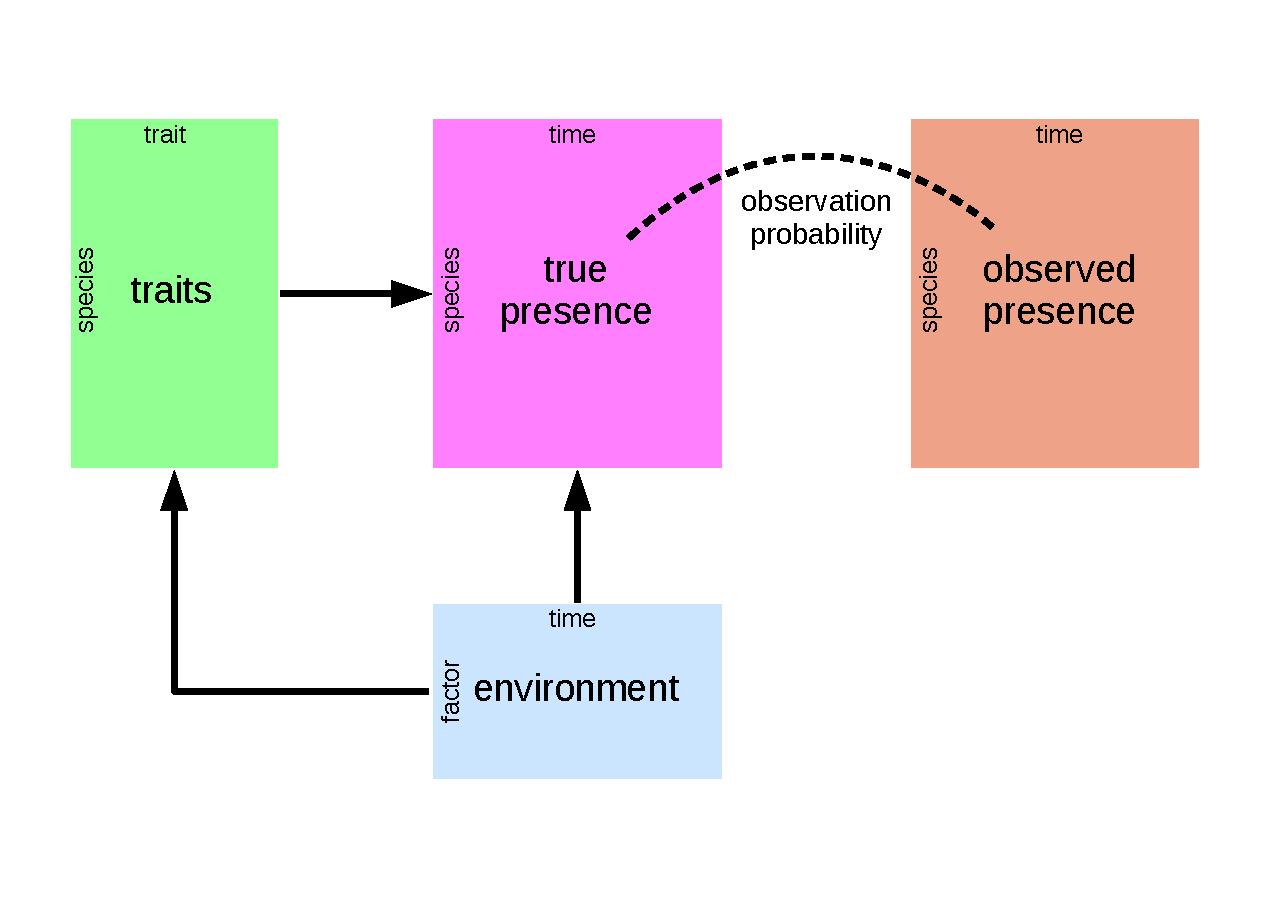
\includegraphics[width=\textwidth,height=0.4\textheight,keepaspectratio=true]{chapter_coping/figure/paleo_fourth_corner}
  \caption[Conceptual diagram of the paleontological fourth-courner problem]{Conceptual diagram of the paleontological fourth corner problem. The observed presence matrix (orange) is the empirical presence/absence pattern for all species for all time points; this matrix is an incomplete observation of the ``true'' presence/absence pattern (purple). The estimated true presence matrix is modeled as a function of both environmental factors over time (blue) and multiple species traits (green). Additionally, the effects of environmental factors on species traits are also modeled, as traits are expected to mediate the effects of a species environmental context. This diagram is based partially on material presented in Brown \textit{et al.} \citep{Brown2014c} and Warton \textit{et al.} \citep{Warton2015a}.}
  \label{fig:concept_fourth_corner}
\end{figure}

My approach to delimiting and assigning mammal functional groups is inspired on the ecocube heuristic used to classify marine invertebrate species by three functional traits \citep{Bush2007,Bambach2007,Bush2011,Bush2012b,Novack-Gottshall2007,Villeger2011} and creodont mammals in a similar fashion \citep{Morlo1999a}. Unique combinations of traits represent ecotypes, which are equivalent to functional groups defined by species functional traits instead of a holistic understanding how a taxon interacts with its environment. In this study, the two functional traits used to define a species' ecotype are dietary (e.g. herbivore, carnivore, etc.) and locomotor category (e.g. arboreal, unguligrade, etc.). Species body mass was also included as a species trait in this analysis, but not as a functional trait for defining ecotypes; instead, its inclusion is principally to control for differences in species dynamics that driven by mass and not ecotype.

The environmental factors included in this study are estimates of global temperature and the changing floral groups present in North America across the Cenozoic \citep{Cramer2011,Graham2011a}. These covariates were chosen because they provide high level characterizations of the environmental context of the entire North American regional species pool for most of the Cenozoic. Importantly, the effects of a species ecotype on diversity are themselves modeled as functions of environmental factors (Fig. \ref{fig:concept_fourth_corner}) allowing for inference as to how a species ecology can mediate selective pressures due to its environmental context. 

All observations, paleontological or modern, are made with uncertainty. With presence/absence data this uncertainty comes from not knowing if an absence is a ``true'' absence or just a failure to observe \citep{Royle2008,Royle2005,Foote1999a,Foote2001,Lloyd2011,Wang2016b}. For paleontological data, the incomplete preservation and sampling of species means that the true times of origination or extinction may not be observed \citep{Foote1999a,Foote2001,Wang2015,Wang2016b}. The model(s) I propose below represent an attempt to translate the verbal/visual model described here (Fig. \ref{fig:concept_fourth_corner}) into a statistical model for estimating the relative diversity of mammal ecotypes over time and how those ecotypes respond to changes to environmental context while taking into account the fundamental incompleteness of the fossil record.

Ultimately, the goals of this analysis are to understand when are different ecotypes enriched or depleted in the North American mammal regional species pool and how these changes in ecotypic diversity are related to changes in species' environmental context. In the analyses done here, many covariates which describe a species' macroecology and its environmental context are considered. In order to analyze this complex and highly structured data set, I developed a hierarchal Bayesian model combining the fourth-corner modeling approach with a model of an observation-occurrence or observation-origination-extinction process. %The complexity and nuance inherent in questions that are focus of this study, it is possible to consider and test a large number of possible hypotheses. The hierarchical Bayesian modeling approach used here is appropriate for mitigating complications arising from both this complexity and the plethora of testable hypotheses (e.g. multiple comparisons, garden of forking paths) \citep{Gelman2013d,Gelman2012a,Gelman2014}.

\section{Materials and Methods}

\subsection{Taxon occurrences and species-level information}
All fossil occurrence information used in this analysis was downloaded from the Paleobiology Database (PBDB). The initial download restricted occurrences to Mammalia observed in North America between the Maastrichtian (72-66 Mya) and Gelasian (2.58-1.8 Mya) stages \citep{Cohen2015}. Occurrences were then further limited to those occurring between 64 and 2 million years ago (Mya); this age restriction was to insure that observation time series lines up with the temperature time series \citep{Cramer2011}. Taxonomic, stratigraphic, and ecological metadata for each occurrence and species was also downloaded. A new download for a raw, unfiltered PBDB datafile following the same criterion used here is available at \texttt{http://goo.gl/2slgeU}. The raw datafile used as a part of this study, along with all code for filtering and manipulating this download is available at \texttt{http://github.com/psmits/coping}.
%https://paleobiodb.org/data1.2/occs/list.csv?datainfo&rowcount&base_name=Mammalia&taxon_reso=species&interval=Maastrichtian,Gelasian&cc=NOA&show=class,genus,ecospace,loc,strat,stratext,lith,acconly. 

After being downloaded, the raw occurrence data was then sorted, cleaned, and manipulated programmatically before analysis. Many species taxonomic assignments as present in the raw PBDB data were updated for accuracy and consistency. For example, species classified in the order Artidodactyla were reclassified as Cetartiodactyla. These re-assignments follow previous work \citep{Smits2015b} which were based on taxonomies present in the Encyclopedia of Life (\texttt{http://eol.org}) and other volumes \citep{Janis1998,Janis2008}. All taxa whose life habit was classified as either volant (i.e. Chiroptera) or aquatic (e.g. Cetacea) were excluded from this analysis because of their lack of direct applicability to the study of terrestrial species pools.

Species ecotype is defined based on a combination of locomotor and diet categories; the goal is to classify species based on the manner with which they interact with their environment. Most mammal species records in the PBDB have life habit (i.e. locomotor category) and dietary category assignments. In order to simplify interpretation, analysis, and per-ecotype sample size these classifications were coarsened in a similar manner to \citep{Smits2015b} following Table \ref{tab:trait_cats2}. The locomotor category was then further broken up to better reflect the diversity of mammal locomotor modes. Ground dwelling species locomotor categories were reassigned based on the ankle posture associated with their taxonomic group, as described in Table \ref{tab:posture} \citep{Carrano1999}. Ankle posture was assumed uniform for all species within a taxonomic group except for those species assigned a non-ground dwelling locomotor category by the PBDB. All species for which it was possible to assign a locomotor category had one assigned, including species for which post-crania are unknown but for which a taxonomic grouping is known. Ground dwelling species which were unable to be reassigned based on ankle posture were excluded from analysis. Finally, ecotype categories with less than 10 total species were excluded, yielding a total of 18 observed ecotypes out of a possible 24.

\begin{table}[ht]
  \centering
  \caption[Species trait reassigments]{Species trait assignments in this study are a coarser version of the information available in the PBDB. Information was coarsened to improve per category sample size.}
  \begin{tabular}[ht]{ l | l | l }
    \hline
    \multicolumn{2}{ c |}{This study} & PBDB categories \\
    \hline
    \multirow{4}{*}{Diet} & Carnivore & Carnivore \\
    & Herbivore & Browser, folivore, granivore, grazer, herbivore. \\
    & Insectivore & Insectivore. \\
    & Omnivore & Frugivore, omnivore. \\ 
    \hline
    \multirow{3}{*}{Locomotor} & Arboreal & Arboreal.\\
    & Ground dwelling & Fossorial, ground dwelling, semifossorial, saltatorial. \\
    & Scansorial & Scansorial. \\
    \hline
  \end{tabular}
  \label{tab:trait_cats2}
\end{table}

\afterpage{\clearpage}

\begin{center}
  \begin{longtable}{ l l l }
    \caption[Posture assignment based on taxonomy]{Ankle posture assignment as based on taxonomy. Assignments are based on \citep{Carrano1999}. Taxonomic groups are presented alphabetically and without reference for the nestedness of families in orders.} \label{tab:posture} \\

    \hline
    Order & Family & Stance \\ \hline
    \endfirsthead
  
    \multicolumn{3}{p{\textwidth}}{{ \bfseries \tablename\ \thetable{} -- continued from previous page}} \\
    \hline Order & Family & Stance \\ \hline
    \endhead
      
    \hline \multicolumn{3}{p{\textwidth}}{{Continued on next page}} \\ \hline
    \endfoot
  
    \hline \hline
    \endlastfoot
  
    & Ailuridae & plantigrade \\ 
    & Allomyidae & plantigrade \\ 
    & Amphicyonidae & plantigrade \\ 
    & Amphilemuridae & plantigrade \\ 
    & Anthracotheriidae & digitigrade \\ 
    & Antilocapridae & unguligrade \\ 
    & Apheliscidae & plantigrade \\ 
    & Aplodontidae & plantigrade \\ 
    & Apternodontidae & scansorial \\ 
    & Arctocyonidae & unguligrade \\ 
    & Barbourofelidae & digitigrade \\ 
    & Barylambdidae & plantigrade \\ 
    & Bovidae & unguligrade \\ 
    & Camelidae & unguligrade \\ 
    & Canidae & digitigrade \\ 
    & Cervidae & unguligrade \\ 
    & Cimolodontidae & scansorial \\ 
    & Coryphodontidae & plantigrade \\ 
    & Cricetidae & plantigrade \\ 
    & Cylindrodontidae & plantigrade \\ 
    & Cyriacotheriidae & plantigrade \\ 
    & Dichobunidae & unguligrade \\ 
    Dinocerata &  & unguligrade \\ 
    & Dipodidae & digitigrade \\ 
    & Elephantidae & digitigrade \\ 
    & Entelodontidae & unguligrade \\ 
    & Eomyidae & plantigrade \\ 
    & Erethizontidae & plantigrade \\ 
    & Erinaceidae & plantigrade \\ 
    & Esthonychidae & plantigrade \\ 
    & Eutypomyidae & plantigrade \\ 
    & Felidae & digitigrade \\ 
    & Florentiamyidae & plantigrade \\ 
    & Gelocidae & unguligrade \\ 
    & Geolabididae & plantigrade \\ 
    & Glyptodontidae & plantigrade \\ 
    & Gomphotheriidae & unguligrade \\ 
    & Hapalodectidae & plantigrade \\ 
    & Heteromyidae & digitigrade \\ 
    & Hyaenidae & digitigrade \\ 
    & Hyaenodontidae & digitigrade \\ 
    & Hypertragulidae & unguligrade \\ 
    & Ischyromyidae & plantigrade \\ 
    & Jimomyidae & plantigrade \\ 
    Lagomorpha &  & digitigrade \\ 
    & Leptictidae & plantigrade \\ 
    & Leptochoeridae & unguligrade \\ 
    & Leptomerycidae & unguligrade \\ 
    & Mammutidae & unguligrade \\ 
    & Megalonychidae & plantigrade \\ 
    & Megatheriidae & plantigrade \\ 
    & Mephitidae & plantigrade \\ 
    & Merycoidodontidae & digitigrade \\ 
    Mesonychia &  & unguligrade \\ 
    & Mesonychidae & digitigrade \\ 
    & Micropternodontidae & plantigrade \\ 
    & Mixodectidae & plantigrade \\ 
    & Moschidae & unguligrade \\ 
    & Muridae & plantigrade \\ 
    & Mustelidae & plantigrade \\ 
    & Mylagaulidae & fossorial \\ 
    & Mylodontidae & plantigrade \\ 
    & Nimravidae & digitigrade \\ 
    & Nothrotheriidae & plantigrade \\ 
    Notoungulata &  & unguligrade \\ 
    & Oromerycidae & unguligrade \\ 
    & Oxyaenidae & digitigrade \\ 
    & Palaeomerycidae & unguligrade \\ 
    & Palaeoryctidae & plantigrade \\ 
    & Pampatheriidae & plantigrade \\ 
    & Pantolambdidae & plantigrade \\ 
    & Periptychidae & digitigrade \\ 
    Perissodactyla &  & unguligrade \\ 
    & Phenacodontidae & unguligrade \\ 
    Primates &  & plantigrade \\ 
    & Procyonidae & plantigrade \\ 
    & Proscalopidae & plantigrade \\ 
    & Protoceratidae & unguligrade \\ 
    & Reithroparamyidae & plantigrade \\ 
    & Sciuravidae & plantigrade \\ 
    & Sciuridae & plantigrade \\ 
    & Simimyidae & plantigrade \\ 
    & Soricidae & plantigrade \\ 
    & Suidae & digitigrade \\ 
    & Talpidae & fossorial \\ 
    & Tayassuidae & unguligrade \\ 
    & Tenrecidae & plantigrade \\ 
    & Titanoideidae & plantigrade \\ 
    & Ursidae & plantigrade \\ 
    & Viverravidae & plantigrade \\ 
    & Zapodidae & plantigrade \\ 
    \hline
  \end{longtable}
\end{center}


Estimates of species mass used in this study were sourced from multiple databases and papers, especially those focusing on similar macroevolutionary or macrecological questions \citep{Tomiya2013,Brook2004a,Freudenthal2013,McKenna2011,Raia2012f,Smith2004}; this is similar to what has been done before \citep{Smits2015b}. When species mass was not available, proxy measures were used and then used to estimate average species mass. For example, given a measurement of a mammal tooth size, it is possible and routine to estimate its mass given some regression equation (Table \ref{tab:mass_esteq}). The PBDB has one or more body part measures for many species. These were used as body size proxies for many species. Mass was log-transformed and then rescaled by first subtracting mean log-mass from all mass estimates, then dividing by two-times its standard deviation; this insures that the magnitude of effects for both continuous and discrete covariates are directly comparable \citep{Gelman2007,Gelman2008}.

In total, 1400 mammal species occurrence histories were included in this study after applying all of the restrictions above.

\begin{table}[ht]
  \centering
  \caption[Equations used to estimate mammal mass]{Regression equations used in this study for estimating body size. Equations are presented with reference to taxonomic grouping, part name, and reference.}
  \begin{tabular}{l | l | l | l}
    \hline
    Group & Equation & log(Measurement) & Source \\
    \hline
    General & \(\log(m) = 1.827x + 1.81\) & lower m1 area &  \cite{Legendre1986} \\
    General & \(\log(m) = 2.9677x - 5.6712\) & mandible length & \cite{Foster2009a} \\
    General & \(\log(m) = 3.68x - 3.83\) & skull length & \cite{Luo2001} \\
    Carnivores & \(\log(m) = 2.97x + 1.681\) & lower m1 length & \cite{VanValkenburgh1990} \\
    Insectivores & \(\log(m) = 1.628x + 1.726\) & lower m1 area & \cite{Bloch1998} \\
    Insectivores & \(\log(m) = 1.714x + 0.886\) & upper M1 area & \cite{Bloch1998} \\
    Lagomorph & \(\log(m) = 2.671x - 2.671\) & lower toothrow area & \cite{Tomiya2013} \\
    Lagomorph & \(\log(m) = 4.468x - 3.002\) & lower m1 length & \cite{Tomiya2013} \\
    Marsupials & \(\log(m) = 3.284x + 1.83\) & upper M1 length & \cite{Gordon2003} \\
    Marsupials & \(\log(m) = 1.733x + 1.571\) & upper M1 area & \cite{Gordon2003} \\
    Rodentia & \(\log(m) = 1.767x + 2.172\) & lower m1 area & \cite{Legendre1986} \\
    Ungulates & \(\log(m) = 1.516x + 3.757\) & lower m1 area & \cite{Mendoza2006} \\
    Ungulates & \(\log(m) = 3.076x + 2.366\) & lower m2 length & \cite{Mendoza2006} \\
    Ungulates & \(\log(m) = 1.518x + 2.792\) & lower m2 area & \cite{Mendoza2006} \\
    Ungulates & \(\log(m) = 3.113x - 1.374\) & lower toothrow length & \cite{Mendoza2006} \\
    \hline
  \end{tabular}
  \label{tab:mass_esteq}
\end{table}


All fossil occurrences from 64 to 2 million years ago (Mya) were binned into 31 two-million year (My) bins. This temporal length was chosen because it is approximately the resolution of the North American mammal fossil record \citep{Alroy1996a,Alroy2000g,Marcot2014,Alroy2009}.



\subsection{Environmental and temporal covariates}
The environmental covariates used in this study are collectively referred to as group-level covariates because they predict the response of a ``group'' of individual-level observations (i.e. species occurrences of an ecotype). Additionally, these covariates are defined for temporal bins and not the species themselves; as such they predict the parts of each species occurrence history. The group-level covariates in this study are two global temperature estimates and the Cenozoic ``plant phases'' defined by Graham \citep{Graham2011a}. 

Global temperature across most of the Cenozoic was calculated from Mg/Ca isotope record from deep sea carbonates \citep{Cramer2011}. Mg/Ca based temperature estimates are preferable to the frequently used \(\delta^{18}\)O temperature proxy \citep{Zachos2001,Zachos2008,Alroy2000g,Figueirido2012} because Mg/Ca estimates do not conflate temperature with ice sheet volume and depth/stratification changes. The former is particularly important to this analysis as the current polar ice-caps appeared and grew during the second half of the Cenozoic. These properties make Mg/Ca based temperature estimates preferable for macroevolutionary and macroecological studies \citep{Ezard2016a}. Two aspects of the Mg/Ca-based temperature curve were included in this analysis: mean and range. Both were calculated as the mean of all respective estimates for each 2 My temporal bins. The distributions of the temperature mean and range estimates were then rescaled by subtracting their respective means from all values and then dividing by twice their respective standard deviations.

\begin{table}
  \centering
  \caption[Plant phase defintions]{Definitions of the start and stop times of the three plant phases used this study as defined by Graham \citep{Graham2011a}.}
  \label{tab:plant_def}
  \begin{tabular}{l c c c}
    \hline
    Plant phase & Phase number & Start & Stop \\
    \hline
    Paleocene-Eocene & 1 & 66 & 50 \\
    Eocene-Miocene & 2 & 50 & 16 \\
    Miocene-Pleistocene & 3 & 16 & 2 \\
  \end{tabular}
\end{table}

The second set of environmental factors included in this study are the Cenozoic plant phases defined by Graham \citep{Graham2011a}. Graham's plant phases are holistic descriptors of the taxonomic composition of 12 ecosystem types, which plants are present at a given time, and the relative modernity of those plant groups with younger phases representing increasingly modern taxa \citep{Graham2011a}. Graham \citep{Graham2011a} defines four intervals from the Cretaceous to the Pliocene, though only three of these intervals take place during the time frame being analyzed. Graham's plant phases was included as a series of ``dummy variables'' encoding the three phases included in this analysis \citep{Gelman2007}; this means that the first phase is synonymous with the intercept and subsequent phases are defined by their differences from the first phase. The temporal boundaries of these plant phases are defined in Table \ref{tab:plant_def}.


\subsection{Modeling species occurrence}
Two different models were used in this study: a pure-presence model and a birth-death model. Both models at their core are hidden Markov models where the latent process has an absorbing state \citep{Allen2011}. The difference between these two models lies in whether the probabilities of a species originating or surviving are considered equal or different (Table \ref{tab:transition}). While there are only two state ``codes'' in a presence-absence matrix (i.e. 0/1), there are in fact three states in a birth-death model: not having originated yet, extant, and extinct. The last of these is the absorbing state, as once a species has gone extinct it cannot re-originate \citep{Allen2011}. Thus, in the transition matrices the probability of an extinct species changing states is 0 (Table \ref{tab:transition}). See below for parameter explanations (Tables \ref{tab:obs_param}, \ref{tab:pres_param}, and \ref{tab:bd_param}).

\begin{table}
  \begin{subtable}[t]{0.45\linewidth}
    \begin{tabular}[c]{ c c | c | c | c | }
      \cline{3-5} 
      & & \multicolumn{3}{ c |}{ State at \(t + 1\)} \\ \cline{3-5}
      & & \(0_{never}\) & 1 & \(0_{extinct}\) \\ \hline
      \multicolumn{1}{| c |}{\multirow{3}{*}{State at \(t\)}}
      & \(0_{never}\) & \(1 - \theta\)  & \(\theta\) & 0 \\ \cline{2-5}
      \multicolumn{1}{| c |}{} & 1 & 0 & \(\theta\) & \(1 - \theta\) \\ \cline{2-5}
      \multicolumn{1}{| c |}{} & \(0_{extinct}\) & 0 & 0 & 1 \\
      \hline
    \end{tabular}
    \caption{Pure-presence}
    \label{tab:pp}
  \end{subtable}
  \begin{subtable}[t]{0.45\linewidth}
    \begin{tabular}[c]{ c c | c | c | c | }
      \cline{3-5} 
      & & \multicolumn{3}{ c |}{ State at \(t + 1\)} \\ \cline{3-5}
      & & \(0_{never}\) & 1 & \(0_{extinct}\) \\ \hline
      \multicolumn{1}{| c |}{\multirow{3}{*}{State at \(t\)}}
      & \(0_{never}\) & \(1 - \pi\)  & \(\pi\) & 0 \\ \cline{2-5}
      \multicolumn{1}{| c |}{} & 1 & 0 & \(\phi\) & \(1 - \phi\) \\ \cline{2-5}
      \multicolumn{1}{| c |}{} & \(0_{extinct}\) & 0 & 0 & 1 \\
      \hline
    \end{tabular}
    \caption{Birth-death}
    \label{tab:bd}
  \end{subtable}
  \caption[Transition matrices for the pure-presence and birth-death models]{Transition matrices for the pure-presence (\ref{tab:pp}) and birth-death (\ref{tab:bd}) models. Both of these models share the core machinery of discrete-time birth-death processes but make distinct assumptions about the equality of originating and surviving (Eq. \ref{eq:pure_presence}, and \ref{eq:birth_death}). Note also that while there are only two state ``codes'' (0, 1), there are in fact three states: never having originated \(0_{never}\), present 1, extinct \(0_{extinct}\) \citep{Allen2011}.}
  \label{tab:transition}
\end{table}


%\subsubsection{Data augmentation}
%All empirical presence/absence observations are potentially incomplete or observed with error. The hidden Markov model at the core of this analysis allows for observed absences to be used meaningfully to estimate the number of unobserved species. Of concern in this analysis is the unknown ``true'' size of the dataset; how many species could have actually been observed? While many species have been observed, the natural incompleteness of all observations, especially in the case of paleontological data, there are obviously many species which were never sampled \citep{Royle2008,Royle2007a}. The inclusion of these augmented species helps with estimation of the total diversity of the system summed over all bins as well as estimation of preservation parameters. % this needs to be checked
%
%Let \(N\) by the total number of observed species, \(M\) be the upper limit of possible species that could have existed in total given some model of species occurrence, and \(N^{\ast}\) is the number of all-zero histories added to the presence absence matrix \(y\) where \(N^{\ast} = M - N\). This approach assumes that \(\hat{N} \sim \text{Binomial}(M, \psi)\) where \(\hat{N}\) is the estimated ``true'' number of species and \(\psi\) is the probability that any augmented species should actually be ``present.'' Because \(M\) is user defined, this approach effectively gives \(\psi\) a uniform prior over \(N\) to \(M\) \citep{Royle2008}. For this study, \(M = \lfloor{1.25 \times N\rfloor}\); this was chosen because experimentation with larger values had little effect on the posterior predictive distributions while dramatically increasing computational time.
%
%Data imputation is the process of estimating missing data for partially observed covariates given the other fully-observed observations and some model \citep{Gelman2007,Rubin1996}, this is simple in a Bayesian context because data are also parameters \citep{Gelman2013d}. Augmented species are fully imputed species and thus have no known mass so a mass estimate must be imputed for each possible species \citep{Royle2012b}. Assuming that mass values for augmented species are from the same distribution as observed species, the distribution of observed mass values are estimated as part of the model and new mass values are then generated from this distribution. This approach is an example of imputing covariate information that is missing completely at random \citep{Gelman2007,Royle2012b}. Because log mass values are rescaled as a part of this study, the body mass distribution is already known (\(\mathcal{N}(0, 0.5)\)) the body mass of the augmented species are generated by simple random draws from this distribution. In addition to body mass information, the augmented species need an ecotype classification. Because these species are completely unknown, they were all classified as ``augmented'' to indicate their unknown biology; it has no biological interpretation. Augmented species were given this classification instead of imputing an ecotype because of the computational cost of estimating the probability of a species being present for each of the 18 possible ecotypes; marginalizing over all possible ecotypes in addition to all possible occurrence histories would dramatically slowdown an already slow posterior inference program (see below for information on what marginalization of species occurrence history means analytically).



\subsubsection{Observation process}
The type of hidden Markov model used in this study has three characteristic probabilities: probability \(p\) of observing a species given that it is present, probability \(\phi\) of a species surviving from one time to another, and probability \(\pi\) of a species first appearing \citep{Royle2008}. In this formulation, the probability of a species becoming extinct is \(1 - \phi\). For the pure-presence model \(\phi = \pi\), while for the birth-death model \(\phi \neq \pi\).

\begin{table}
  \centering
  \caption{Parameters for the observation process part of the hidden Markov model.}
  \begin{tabular}{c l l}
    Parameter & dimensions & explanation \\
    \hline
    \(y\) & \(N \times T\) & observed species presence/absence \\
    \(z\) & \(N \times T\) & ``true'' species presence/absence \\
    \(p\) & \(T\) & probability of observing a species that is present at time \(t\) \\
    \(m\) & \(N\) & species log mass, rescaled \\
    \(\alpha_{0}\) & 1 & average log-odds of \(p\) \\ % when mass = 0
    \(\alpha_{1}\) & 1 & change in average log-odds of \(p\) per change mass \\
    \(r\) & \(T\) & difference from \(\alpha_{0}\) associated with time \(t\) \\
    \(\sigma\) & 1 & standard deviation of \(r\) \\
  \end{tabular}
  \label{tab:obs_param}
\end{table}

The probability \(p\) of observing a species that is present is modeled as a logistic regression with a time-varying intercept and species mass as a covariate. The effect of species mass on \(p\) was assumed linear and constant over time. These assumptions are reflected in the structure of this part of the model being presented here: 
\begin{equation}
  \begin{aligned}
    y_{i, t} &\sim \text{Bernoulli}(p_{i, t} z_{i, t}) \\
    p_{i, t} &= \text{logit}^{-1}(\alpha_{0} + \alpha_{1} m_{i} + r_{t}) \\ 
    r_{t} &\sim \mathcal{N}(0, \sigma). \\
  \end{aligned}
  \label{eq:obs_model}
\end{equation}
The parameters associated with Equation \ref{eq:obs_model} are described in Table \ref{tab:obs_param}.


\subsubsection{Pure-presence process}
For the pure-presence model there is only a single probability dealing with the presence of a species \(\theta\) (Table \ref{tab:pp}). This probability was modeled as multi-level logistic regression with both species-level and group-level covariates \citep{Gelman2007,Gelman2013d}. The parameters associated with the pure-presence model are presented in Table \ref{tab:pres_param}, and the full sampling statement in Equation \ref{eq:pure_presence}.

\begin{table}
  \centering
  \caption{Parameters for the model of occurrence in the pure-presence model}
  \begin{tabular}{c l l}
    Parameter & dimensions & explanation \\
    \hline
    \(z\) & \(N \times T\) & ``true'' species presence/absence \\
    \(\theta\) & \(N \times T - 1\) & probability of \(z = 1\) \\
    \(a\) & \(T - 1 \times D\) & ecotype-varying intercept; mean value of log-odds of \(\theta\) \\
    \(m\) & \(N\) & species log mass, rescaled \\
    \(b_{1}\) & 1 & effect of species mass on log-odds of \(\theta\) \\
    \(b_{2}\) & 1 & effect of species mass, squared, on log-odds of \(\theta\) \\
    \(U\) & \(T \times D\) & matrix of group-level covariates \\
    \(\gamma\) & \(U \times D\) & matrix of group-level regression coefficients \\
    \(\Sigma\) & \(D \times D\) & covariance matrix of \(a\) \\
    \(\Omega\) & \(D \times D\) & correlation matrix of \(a\) \\
    \(\tau\) & \(D\) & vector of standard deviations for each ecotype \(a_{d}\) \\
  \end{tabular}
  \label{tab:pres_param}
\end{table}

Species mass was included as a covariate with two regression coefficients allowing for a quadratic relationship with log-odds of occurrence. Because the distribution of mammal species body mass is unimodal and approximately log-normal \citep{Smith2004}, I assume that species of intermediate body size will be more common than species of very large or very small mass. These assumptions are also reflected in the choice of priors for \(b_{1}\) and \(b_{2}\) where the latter is given a weakly informative prior with most of its density below 0 (Eq. \ref{eq:pure_presence}).

The values of each ecotype's intercept are themselves modeled as regressions using the group-level covariates associated with environmental context. Each of these regressions has an associated variance of possible values of each ecotype's intercept \citep{Gelman2007}. In addition, the covariances between ecotype intercepts, given this group-level regression, are modeled \citep{Gelman2007}. The prior choice for the covariance matrix separates it into a vector of scales \(\tau\) and a correlation matrix \(\Omega\). The elements of the former are given weakly informative, independent half-Normal priors while the latter was given a weakly informative LKJ prior as recommended in the Stan manual \citep{StanDevelopmentTeam2016}.

All parameters not modeled elsewhere were given weakly informative priors \citep{Gelman2013d,McElreath2016,StanDevelopmentTeam2016}. Weakly informative means that priors do not necessarily encode actual prior information but instead help regularize or weakly constrain posterior estimates. These priors have a concentrated probability density around and near zero; this has the effect of tempering our estimates and help prevent overfitting the model to the data \citep{Gelman2013d,McElreath2016,StanDevelopmentTeam2016}. The general line of thinking behind this approach is that a result of 0 or ``no effect'' is more preferable to a wrong or extremely weak result.

\begin{equation}
  \begin{split}
    y_{i, t} &\sim \text{Bernoulli}(p_{i, t} z_{i, t}) \\
    p_{i, t} &= \text{logit}^{-1}(\alpha_{0} + \alpha_{1} m_{i} + r_{t}) \\ 
    r_{t} &\sim \mathcal{N}(0, \sigma) \\
    z_{i, 1} &\sim \text{Bernoulli}(\rho) \\
    z_{i, t} &\sim \text{Bernoulli}(\theta_{i, t}) \\
    \theta_{i, t} &= \text{logit}^{-1}(a_{t, j[i]} + b_{1} m_{i} + b_{2} m_{i}^{2}) \\
    a &\sim \text{MVN}(u \gamma, \Sigma) \\
    \Sigma &= \text{diag}(\tau) \Omega \text{diag}(\tau) \\
  \end{split}
  \begin{split}
    \alpha_{0} &\sim \mathcal{N}(0, 1) \\
    \alpha_{1} &\sim \mathcal{N}(1, 1) \\
    \sigma &\sim \mathcal{N}^{+}(1) \\
    b_{1} &\sim \mathcal{N}(0, 1) \\
    b_{2} &\sim \mathcal{N}(-1, 1) \\
    \gamma &\sim \mathcal{N}(0, 1) \\
    \tau &\sim \mathcal{N}^{+}(1) \\
    \Omega &\sim \text{LKJ}(2) \\
  \end{split}
  \label{eq:pure_presence}
\end{equation}


\subsubsection{Birth-death process}
In the birth-death version of the model, \(\phi \neq \pi\) and so each of these probabilities is modeled separately but each is handled in a similar manner to how \(\theta\) is modeled in the pure-presence model (Eq. \ref{eq:pure_presence}, Table \ref{tab:bd}). The parameters associated with the birth-death presence model are presented in Table \ref{tab:bd_param} and the full sampling statement, including observation (Eq. \ref{eq:obs_model}), is described in Equation \ref{eq:birth_death}:
\begin{equation}
  \begin{split}
    y_{i, t} &\sim \text{Bernoulli}(p_{i, t} z_{i, t}) \\
    p_{i, t} &= \text{logit}^{-1}(\alpha_{0} + \alpha_{1} m_{i} + r_{t}) \\ 
    r_{t} &\sim \mathcal{N}(0, \sigma) \\
    \alpha_{0} &\sim \mathcal{N}(0, 1) \\
    \alpha_{1} &\sim \mathcal{N}(1, 1) \\
    \sigma &\sim \mathcal{N}^{+}(1) \\
    z_{i, 1} &\sim \text{Bernoulli}(\phi_{i, 1}) \\
    z_{i, t} &\sim \text{Bernoulli}\left(z_{i, t - 1} \pi_{i,t} + \sum_{x = 1}^{t}(1 - z_{i, x}) \phi_{i,t}\right) \\
    \phi_{i, t} &= \text{logit}^{-1}(a^{\phi}_{t, j[i]} + b^{\phi}_{1} m_{i} + b^{\phi}_{2} m_{i}^{2}) \\
    \pi_{i, t} &= \text{logit}^{-1}(a^{\pi}_{t, j[i]} + b^{\pi}_{1} m_{i} + b^{\pi}_{2} m_{i}^{2}) \\
    a^{\phi} &\sim \text{MVN}(U \gamma^{\phi}, \Sigma^{\phi}) \\
    a^{\pi} &\sim \text{MVN}(U \gamma^{\pi}, \Sigma^{\pi}) \\
  \end{split}
  \begin{split}
    \Sigma^{\phi} &= \text{diag}(\tau^{\phi}) \Omega^{\phi} \text{diag}(\tau^{\phi}) \\
    \Sigma^{\pi} &= \text{diag}(\tau^{\pi}) \Omega^{\pi} \text{diag}(\tau^{\pi}) \\
    \rho &\sim \text{U}(0, 1) \\
    b^{\phi}_{1} &\sim \mathcal{N}(0, 1) \\
    b^{\pi}_{1} &\sim \mathcal{N}(0, 1) \\
    b^{\phi}_{2} &\sim \mathcal{N}(-1, 1) \\
    b^{\pi}_{2} &\sim \mathcal{N}(-1, 1) \\
    \gamma^{\phi} &\sim \mathcal{N}(0, 1) \\
    \gamma^{\pi} &\sim \mathcal{N}(0, 1) \\
    \tau^{\phi} &\sim \mathcal{N}^{+}(1) \\
    \tau^{\pi} &\sim \mathcal{N}^{+}(1) \\
    \Omega^{\phi} &\sim \text{LKJ}(2) \\
    \Omega^{\pi} &\sim \text{LKJ}(2). \\
  \end{split}
  \label{eq:birth_death}
\end{equation}


\begin{table}
  \centering
  \caption{Parameters for the model of presence in the pure-presence model}
  \begin{tabular}{c l l}
    Parameter & dimensions & explanation \\
    \hline
    \(z\) & \(N \times T\) & ``true'' species presence/absence \\
    \(\phi\) & \(N \times T\) & probability of \(z_{\textunderscore, t} = 1 | z_{\textunderscore, t - 1} = 0 \); origination \\
    \(\pi\) & \(N \times T - 1\) & probability of \(z_{\textunderscore, t} = 1 | z_{\textunderscore, t - 1} = 1 \); survival \\
    \(a^{\phi}\) & \(T - 1 \times D\) & ecotype-varying intercept; mean value of log-odds of \(\theta\) \\
    \(a^{\pi}\) & \(T - 1 \times D\) & ecotype-varying intercept; mean value of log-odds of \(\theta\) \\
    \(m\) & \(N\) & species log mass, rescaled \\
    \(b^{\phi}_{1}\) & 1 & effect of species mass on log-odds of \(\phi\) \\
    \(b^{\pi}_{1}\) & 1 & effect of species mass on log-odds of \(\pi\) \\
    \(b^{\phi}_{2}\) & 1 & effect of species mass, squared, on log-odds of \(\phi\) \\
    \(b^{\pi}_{2}\) & 1 & effect of species mass, squared, on log-odds of \(\pi\) \\
    \(U\) & \(T \times D\) & matrix of group-level covariates \\
    \(\gamma^{\phi}\) & \(U \times D\) & matrix of group-level regression coefficients \\
    \(\gamma^{\pi}\) & \(U \times D\) & matrix of group-level regression coefficients \\
    \(\Sigma^{\phi}\) & \(D \times D\) & covariance matrix of \(a^{\phi}\) \\
    \(\Sigma^{\pi}\) & \(D \times D\) & covariance matrix of \(a^{\pi}\) \\
    \(\Omega^{\phi}\) & \(D \times D\) & correlation matrix of \(a^{\phi}\) \\
    \(\Omega^{\pi}\) & \(D \times D\) & correlation matrix of \(a^{\pi}\) \\
    \(\tau^{\phi}\) & \(D\) & vector of standard deviations for each ecotype \(a^{\phi}_{d}\) \\
    \(\tau^{\pi}\) & \(D\) & vector of standard deviations for each ecotype \(a^{\pi}_{d}\) \\
  \end{tabular}
  \label{tab:bd_param}
\end{table}

Similar to the pure-presence model, both \(\phi\) and \(\pi\) are modeled as logistic regressions with varying intercept and one covariate associated with two parameters. The possible relationships between mass and both \(\phi\) and \(\pi\) are reflected in the parameterization of the model and choice of priors (Eq. \ref{eq:birth_death}).

The intercepts of \(\phi\) and \(\pi\) both vary by species ecotype and those values are themselves the product of group-level regression using environmental factors as covariates (Eq. \ref{eq:birth_death}); this is identical to the pure presence model (Eq. \ref{eq:pure_presence}).


\subsection{Posterior inference and model adequacy}
Computer programs that implement joint posterior inference for the above models (Eqs. \ref{eq:pure_presence}, \ref{eq:birth_death}) were written in the probabilistic programming language Stan \citep{StanDevelopmentTeam2016}. Both models feature a large matrix of latent discrete parameters \(z\) (Tables \ref{tab:obs_param}, \ref{tab:pres_param}, \ref{tab:bd_param}; Eqs. \ref{eq:obs_model}, \ref{eq:pure_presence}, \ref{eq:birth_death}). All methods for posterior inference implemented in Stan are derivative-based; this causes complications for actually implementing the above models, because integers do not have derivatives. Instead of implementing a latent discrete parameterization, the log posterior probabilities of all possible states of the latent parameters \(z\) were calculated and summed (i.e. marginalized). 

Species durations at minimum range through from a species first appearance to their last appearance in the fossil record, but the incompleteness of all observations means that the actual times of origination and extinction are unknown. The marginalization approach used here means that the probabilities of all possible histories for a species are calculated, from the end members of the species having existed for the entire study interval and the species having only existed between the directly observed first and last appearances to all possible intermediaries (Fig \ref{fig:margin_concept}) \citep{StanDevelopmentTeam2016}. This process is identical, language-wise, to assuming range-through and then estimating the possibility of all possible range extension due to incomplete sampling. % this probably needs a figure to explain.

\begin{figure}[ht]
  \centering
  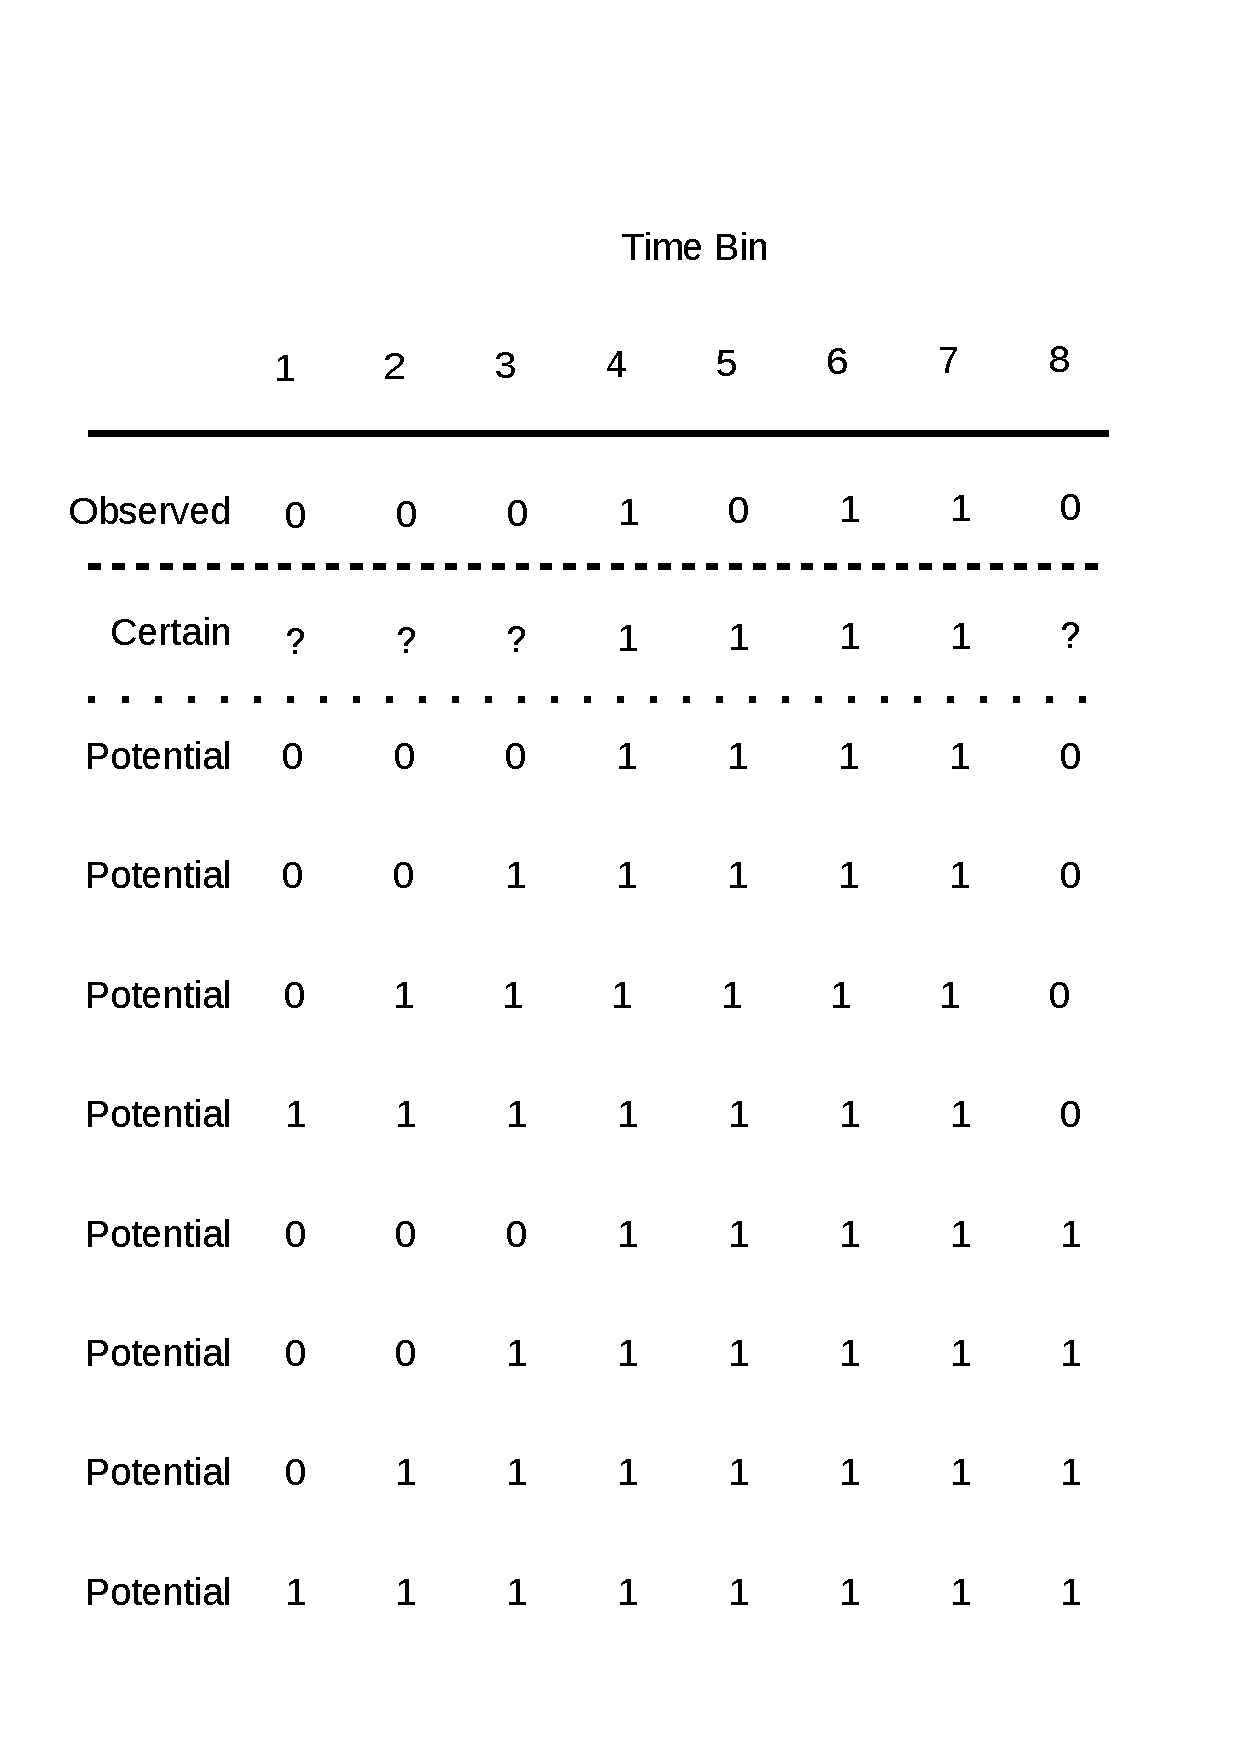
\includegraphics[height=0.4\textheight, width=\textwidth, keepaspectratio=true]{chapter_coping/figure/margin}
  \caption[Conceptual figure of all possible occurrence histories for an observed species]{Conceptual figure of all possible occurrence histories for an observed species. The first row represents the observed presence/absence pattern for a single species at eight time points. The second row corresponds to the known aspects of the ``true'' occurrence history of that species. The remaining rows correspond to all possible occurrence histories that are consistent with the observed data. By marginalizing over all possible occurrence histories, the probability of each potential history is estimated. The process of parameter marginalization is described in the text.}
  \label{fig:margin_concept}
\end{figure}


% Stan
%   version 2.9.0
%   marginalize over latent discrete parameters
%     keeping in mind that species HAVE to range through
%     sum of the log probability for all possible configutations
%     along with the sampling probability given those combinations as well
%     see code for implementation? 
%       it is kind of an annoying amount of math to write up

The combined size of the dataset and large number of parameters in both models (Eqs. \ref{eq:pure_presence}, \ref{eq:birth_death}), specifically the total number of latent parameters that are the matrix \(z\), means that stochastic approximate posterior inference is computationally very slow even using NUTS based HMC as implemented in Stan \citep{StanDevelopmentTeam2016}. Instead, an approximate Bayesian approach was used: variational inference. A recently developed automatic variational inference algorithm called ``automatic differention variational inference'' (ADVI) is implemented in Stan and was used here \citep{Kucukelbir2015,StanDevelopmentTeam2016}. ADVI assumes that the posterior is Gaussian but still yields a true Bayesian posterior; this assumption is similar to quadratic approximation of the likelihood function commonly used in maximum likelihood based inference \citep{McElreath2016}. The principal limitation of assuming the joint posterior is Gaussian is that the true topology of the log-posterior isn't estimated; this is a particular burden for scale parameters which are bounded to be positive (e.g. standard deviation).

Of additional concern for posterior inference is the partial identifiability of observation parameters \(p_{t = 1}\) and \(p_{t = T}\) \citep{Royle2008}. This issue means that the estimates of sampling probabilities at the ``edges'' of the time series cannot fully be estimated because there are no known ``gaps'' in species occurrence histories that are guaranteed to be filled. Instead, the values of the first and final columns of the ``true'' presence-absence matrix \(z\) for thos observations that do not already have presences in the observed presence-absence matrix \(y\) cannot be estimated \citep{Royle2008}. The hierarchical modeling approach used here helps mitigate this problem by pulling the values of \(p_{t = 1}\) and \(p_{t = T}\) towards the overall mean of \(p\) \citep{Gelman2013d}, and in fact this approach might be more analytically sound than the more ad-hoc approaches that are occasionally used to overcome this hurdle \citep{Royle2008}. Additionally, because \(p_{t = 1}\) and \(p_{t = T}\) are only partially identifiable, estimates of occurrence \(\theta\) and origination \(\phi\) at \(t = 1\) and estimates of \(\theta\), \(\phi\) and survival \(\pi\) at \(t = T\) may suffer from similar edge effects. Again, the hierarchical modeling approach used here may help correct for this reality by drawing these estimates towards the overall means of those parameters.


After fitting both models (Eqs. \ref{eq:pure_presence}, \ref{eq:birth_death}) using ADVI, model adequacy and quality of fit were assessed using a posterior predictive check \citep{Gelman2013d}. By simulating 100 theoretical data sets from the posterior estimates of the model parameters and the observed covariate information the congruence between predictions made by the model and the observed empirical data can be assessed. These datasets are simulated by starting with the observed states of the presence-absence matrix at \(t = 1\); from there, the time series roll forward as stochastic processes with covariate information given from the empirical observations. Importantly, this is fundamentally different from observing the posterior estimates of the ``true'' presence-absence matrix \(z\). The posterior predictive check used in this study is to compare the observed average number of observations per species to a distribution of simulated averages; if the empirically observed value sits in the middle of the distribution then the model can be considered adequate in reproducing the observed number of occurrences per species. 

The ADVI assumption of a purely Gaussian posterior limits the utility and accuracy of the posterior predictive checks because parameter estimates do not reflect the true posterior distribution and are instead just an approximation \citep{Gelman2013d}. Because of this, posterior predictive estimates are themselves only approximate checks of model adequacy. The posterior predictive check that is used in this study focuses on mean occurrence and not to any scale parameters that might be most affected by the ADVI assumptions.


Given parameter estimates, diversity and diversification rates are estimated through posterior predictive simulations. Given the observed presence-absence matrix \(y\), estimates of the true presence-absence matrix \(z\) can be simulated and the distribution of possible occurrence histories can be analyzed. This is conceptually similar to marginalization where the probability of each possible occurrence history is estimated (Fig. \ref{fig:margin_concept}), but now these occurrence histories are generated relative to their estimated probabilities.

The posterior distribution of \(z\) gives the estimate of standing diversity \(N^{stand}_{t}\) for all time points as 
\begin{equation}
  N^{stand}_{t} = \sum_{i = 1}^{M} z_{i, t}.
  \label{eq:stand_est}
\end{equation}
Given estimates of \(N^{stand}\) for all time points, the estimated number of originations \(O_{t}\) is estimated as 
\begin{equation}
  O_t = \sum_{i = 1}^{M} z_{i, t} = 1 | z_{i, t - 1} = 0
  \label{eq:orig_est}
\end{equation}
and number of extinctions \(E_{t}\) estimated as
\begin{equation}
  E_{t} = \sum_{i = 1}^{M} z_{i, t} = 0 | z_{i, t - 1} = 1.
  \label{eq:death_est}
\end{equation}
Per-capita growth \(D^{rate}\), origination \(O^{rate}\) and extinction \(E^{rate}\) rates are then calculated as
\begin{equation}
  \begin{aligned}
    O^{rate}_{t} &= \frac{O_t}{N^{stand}_{t - 1}} \\
    E^{rate}_{t} &= \frac{E_t}{N^{stand}_{t - 1}} \\
    D^{rate}_{t} &= O^{rate}_{t} - E^{rate}_{t}. \\
  \end{aligned}
  \label{eq:per_capita_est}
\end{equation}

% silly transforms using the poisson distribution aren't necessary if you just do the posterior simulations.
% discuss this in the discussion and not this section?

\section{Results}

The results of the analyses described above take one of two forms: direct inspection of parameter posterior estimates from both models, and downstream estimates of diversity and diversification rates based on posterior predictive simulations from the birth-death model because this model has a better fit to the observed occurrence information.

\subsection{Comparison of estimates from the pure-presence and birth-death models}

% look at the posterior predictive checks
%   which model has better fit
%   what does that mean?


\begin{figure}[ht]
  \begin{subfigure}[b]{0.45\textwidth}
    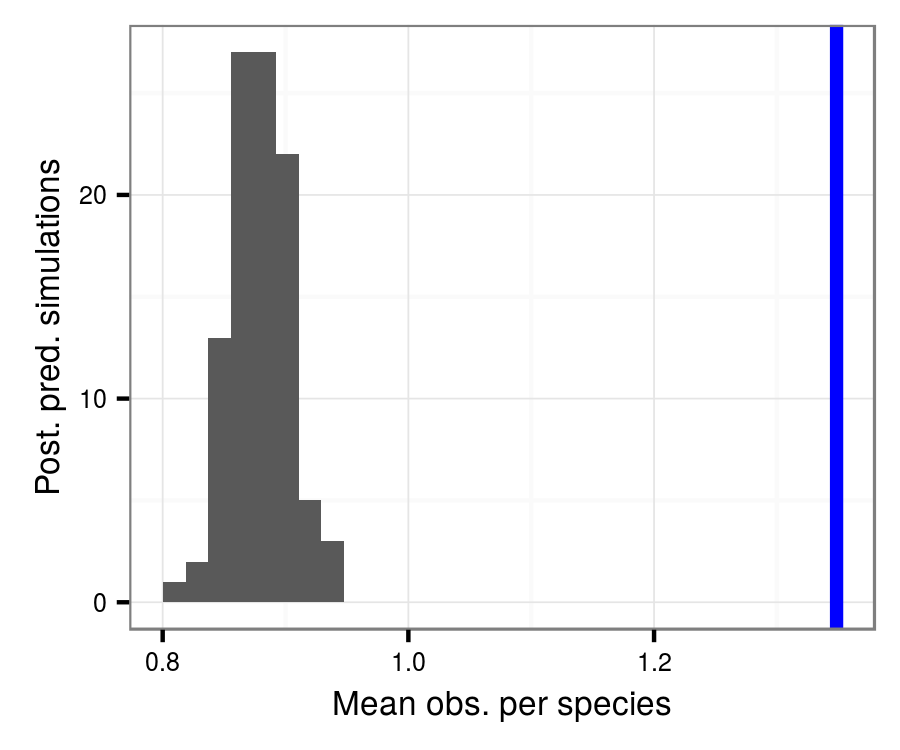
\includegraphics[width=\textwidth,height=0.3\textheight,keepaspectratio=true]{chapter_coping/figure/pred_occ}
    \caption{Pure-presence model}
    \label{fig:ppc_pure_presence}
  \end{subfigure}
  \begin{subfigure}[b]{0.45\textwidth}
    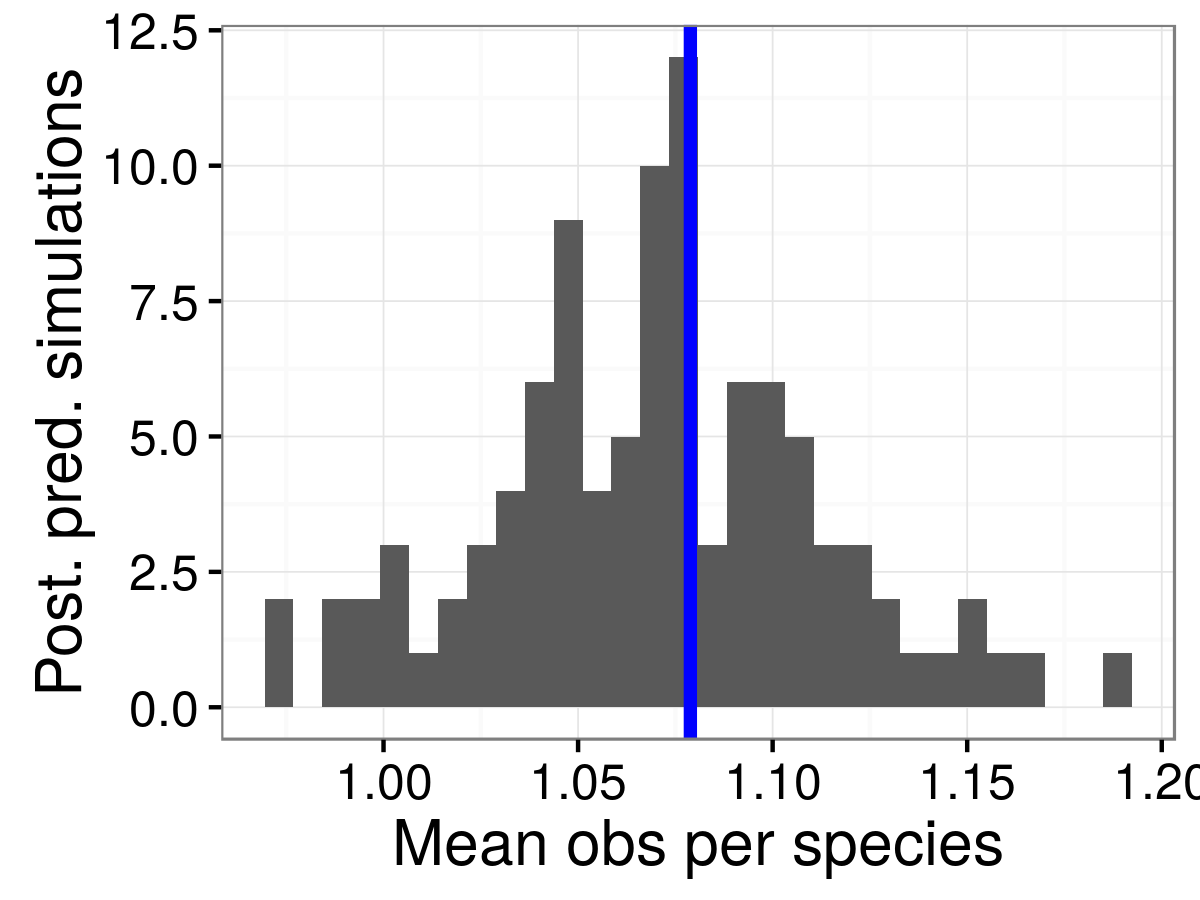
\includegraphics[width=\textwidth,height=0.3\textheight,keepaspectratio=true]{chapter_coping/figure/pred_occ_bd}
    \caption{Birth-death model}
    \label{fig:ppc_birth_death}
  \end{subfigure}
  \caption[Posterior predictive check of average occurrence]{Comparison of the average observed number of occurrences per species (blue line) to the average number of occurrences from 100 posterior predictive datasets using the posterior estimates from the pure-presence and birth-death models.}
  \label{fig:ppc}
\end{figure}

Comparison of the posterior predictive results from the pure-presence and birth-death models reveals a striking difference in performance of either model to predict the structure of the underlying data (Fig. \ref{fig:ppc}). The simulated datasets generated from the birth-death model are clearly able to better reproduce the observed average number of occurrence than the pure-presence model which underestimates the observed average number of occurrences. This result means that inferences based on the birth-death model are more likely to be representative of the underlying data than inferences based on the pure-presence model. Further inspection of the posterior parameter estimates from both models gives further insight into the resins for this difference in posterior predictive results \citep{Gelman2013d}. 

Increases in the occurrence probability of an ecotype is interpreted as an increase in the commonness of that ecotype in the species pool. In turn, decreases in the occurrence probability of an ecotype are interpreted to a decrease in the commonness of that ecotype in the species pool. Additionally, when the uncertainty surrounding a probability estimate is very high, as with arboreal insectivores, this is interpreted as complete separation which means that that ecotype has most likely all but disappeared from the species pool \citep{Gelman2007}. In logistic regression, high uncertainty in the estimates of the underlying log-odds of occurrence, origination, or survival tends to indicate extreme rarity or complete absence of the specific ecotype. The latter is called complete separation and occurs when there is no uncertainty in the effect of a covariate on presence/absence. The problem of complete separation is mitigated by the hierarchical modeling strategy used here \citep{Gelman2013d,Gelman2007,McElreath2016}.

Estimates of occurrence probability estimated from the pure-presence model and estimates of origination probability from the birth-death model are broadly similar (Fig. \ref{fig:eco_occur}, \ref{fig:eco_origin}); this is not the case for the survival probability estimates (Fig. \ref{fig:eco_survival}). This result supports the idea that changes to the North American regional species pool is more likely due to changes in origination than extinction, a result to which I will return to later in the discussion of per-capita diversification, origination, and extinction rates. For most ecotypes, occurrence and origination probability estimates increase with time (Fig. \ref{fig:eco_origin}). This makes sense given that, over time, all species that have at least one observed occurrence must have had that occurrence by the last time point, so our certainty in a species occurring must increase with time. Notably, ecotypes with arboreal components do not appear to follow the same pattern as most other ecotypes; instead, origination probabilities appear relatively flat with high posterior variance for most of the Cenozoic. For most ecotypes, occurrence or origination probability is estimated with less uncertainty than its estimate of survival probability (Fig. \ref{fig:eco_occur}, \ref{fig:eco_origin}, \ref{fig:eco_survival}). 



\begin{figure}[ht]
  \centering
  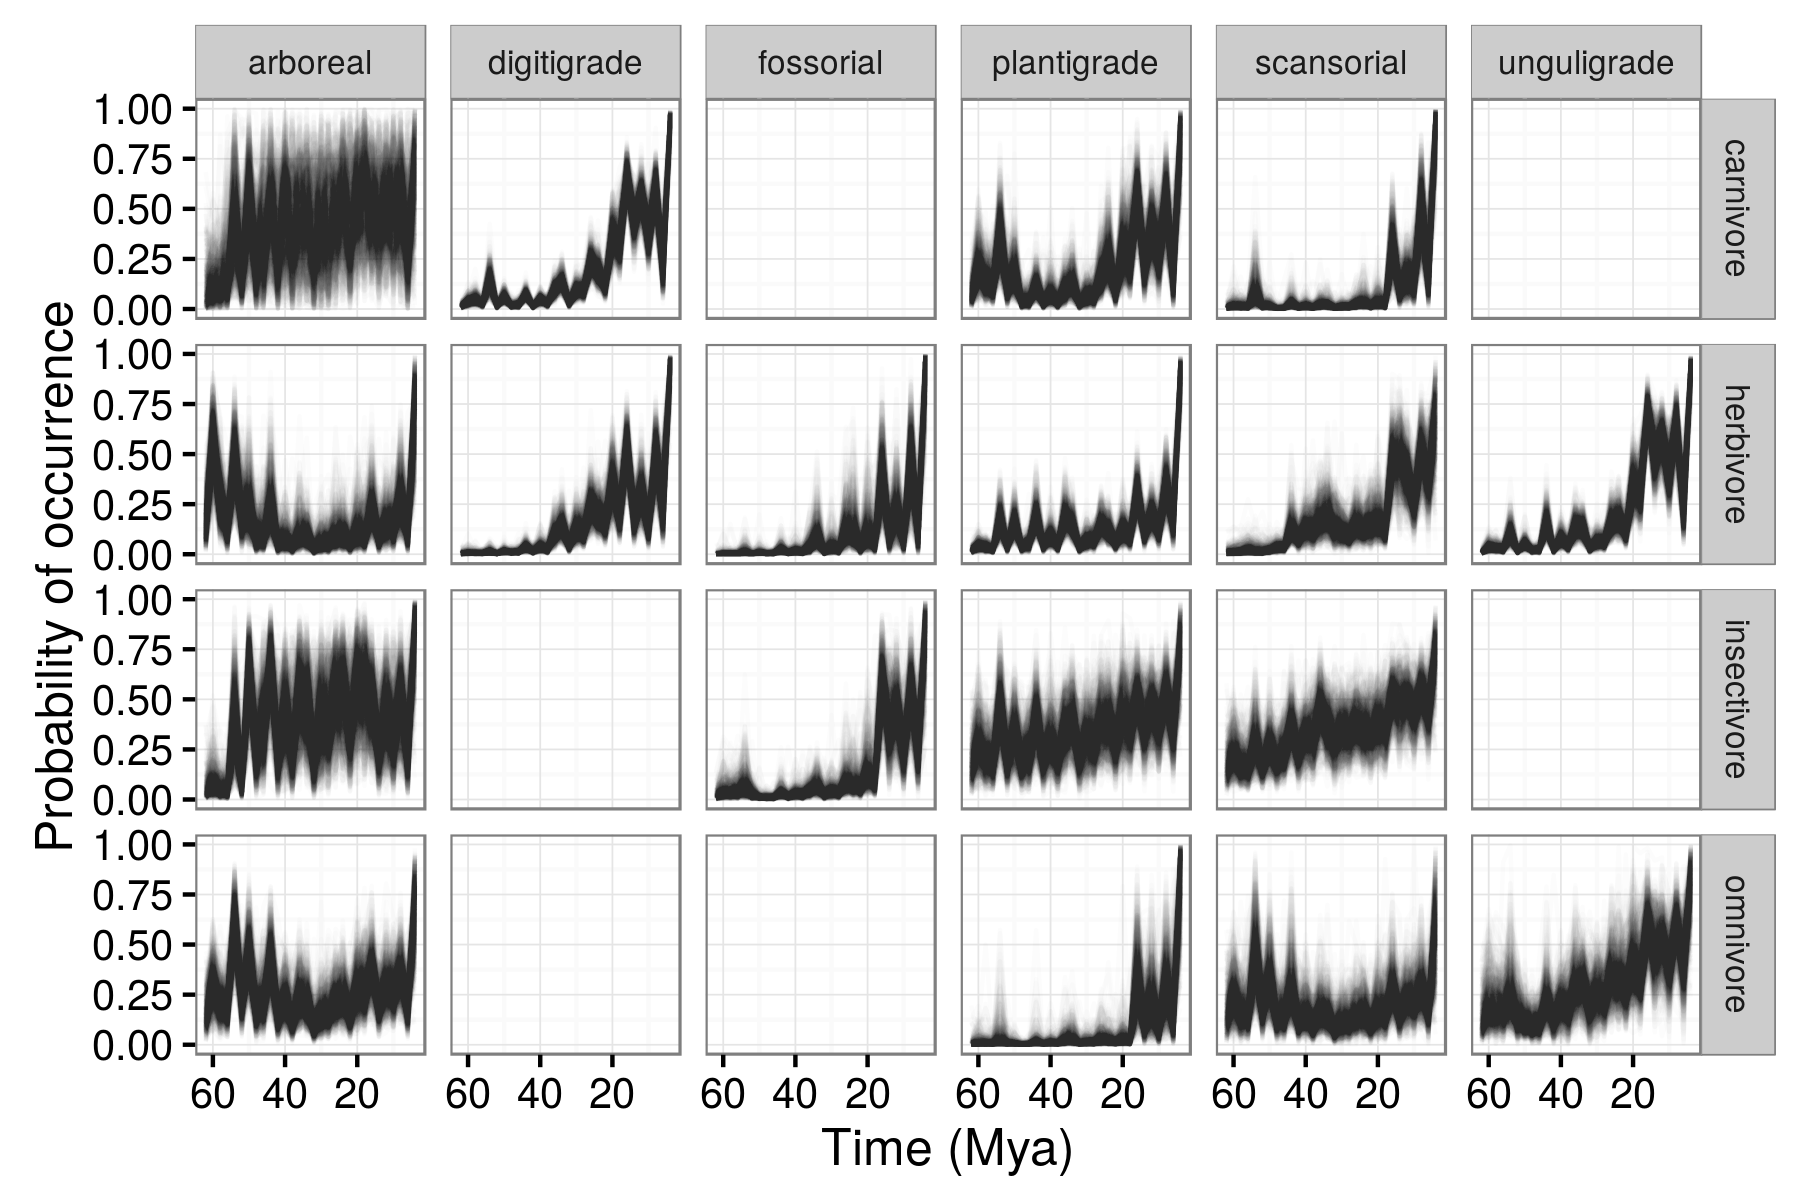
\includegraphics[width=\textwidth,height=0.4\textheight,keepaspectratio=true]{chapter_coping/figure/ecotype_occurrence}
  \caption[Ecotype occurrence probability estimated from the pure-presence model]{Probability of a mammal ecotype occurring over time as estimated from the pure-presence model. Each panel depicts 100 random samples from the model's posterior. The columns are by locomotor category and rows by dietary category; their intersections are the observed and analyzed ecotypes. Panels with no lines are ecotypes not observed in the dataset.}
  \label{fig:eco_occur}
\end{figure}

\begin{figure}[ht]
  \centering
  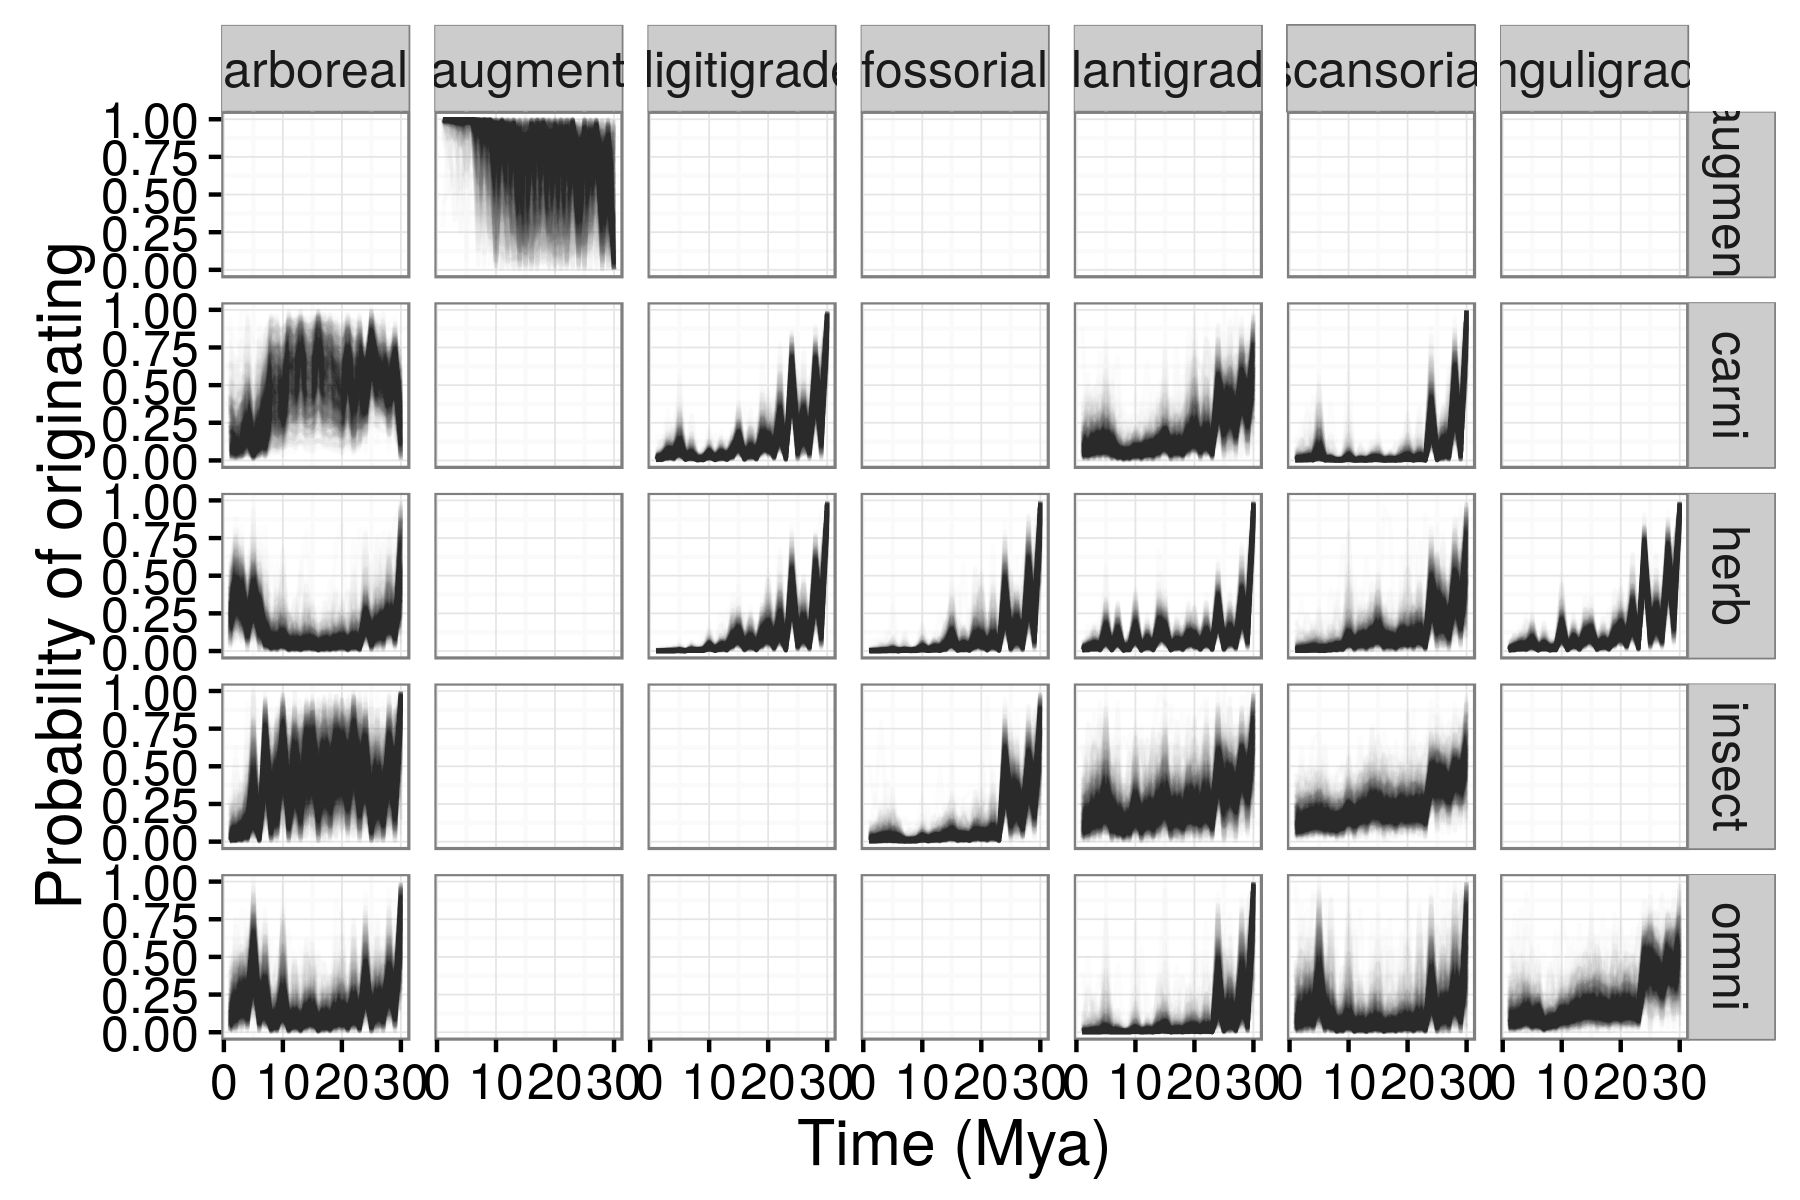
\includegraphics[width=\textwidth,height=0.4\textheight,keepaspectratio=true]{chapter_coping/figure/ecotype_origin_bd}
  \caption[Ecotype origination probability estimated from the birth-death model]{Probability of a mammal ecotype origination probabliities at each time point as estimated from the birth-death model. Each panel depicts 100 random samples from the model's posterior. The columns are by locomotor category and rows by dietary category; their intersections are the observed and analyzed ecotypes. Panels with no lines are ecotypes not observed in the dataset.}
  \label{fig:eco_origin}
\end{figure}

\begin{figure}[ht]
  \centering
  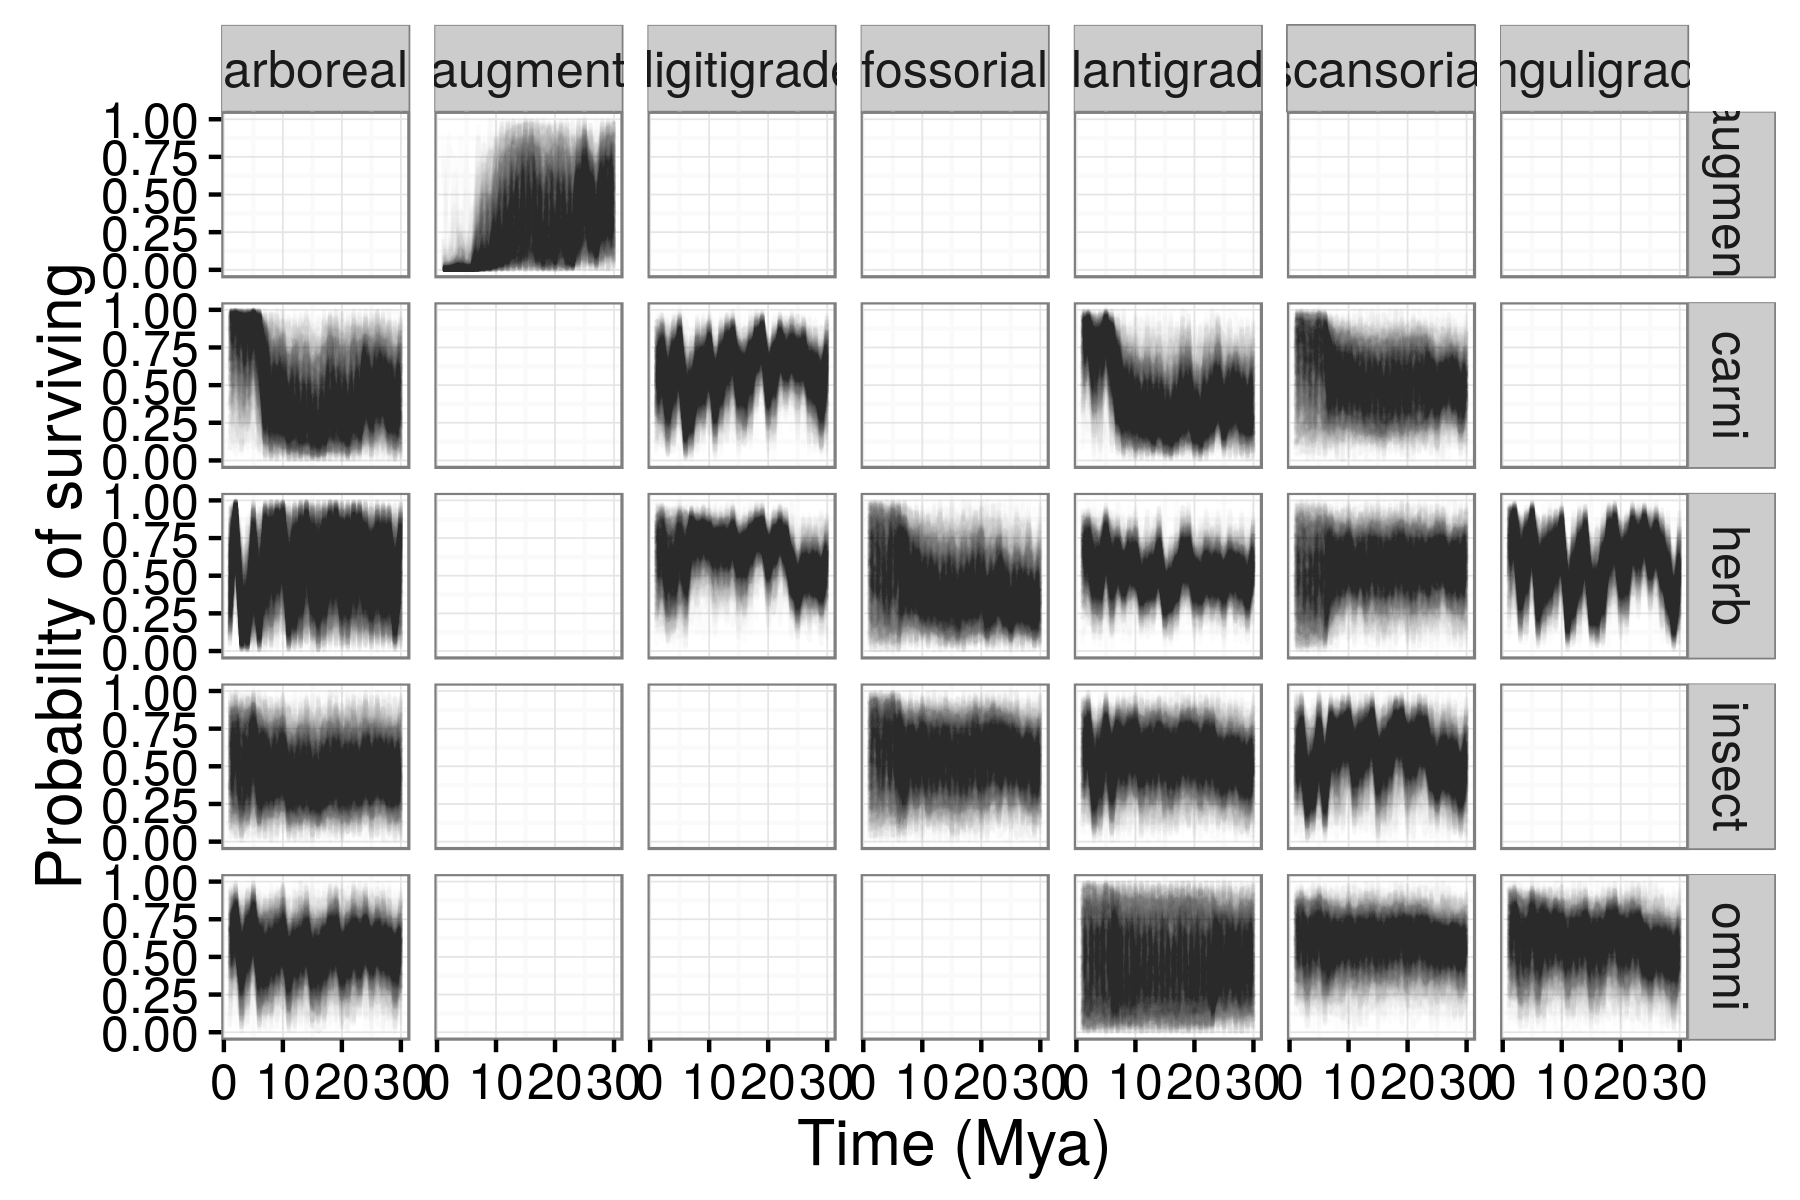
\includegraphics[width=\textwidth,height=0.4\textheight,keepaspectratio=true]{chapter_coping/figure/ecotype_survival_bd}
  \caption[Ecotype survival probability estimated from the birth-death model]{Probability of a mammal ecotype survival probabilities at each time point as estimated from the birth-death model. Each panel depicts 100 random samples from the model's posterior. The columns are by locomotor category and rows by dietary category; their intersections are the observed and analyzed ecotypes. Panels with no lines are ecotypes not observed in the dataset.}
  \label{fig:eco_survival}
\end{figure}


The pure-presence and birth-death models have similar estimates of the relationship between species mass and the probability of sampling a species that is present (Fig. \ref{fig:mass_preserve}). For both models this relationship is at least weakly positive, which means that as species body mass increases it is expected that they are more likely to be sampled if present. The estimated relationship from the pure-presence model is with greater uncertainty than that from the birth-death model (Fig. \ref{fig:mass_preserve}). These results are consistent with the intuition that larger fossils are easier to sample because they are more visible to the eye. In turn, this means that the observed occurrence histories of small bodied species are more likely to have gaps, where \(y = 0\) for that species the true state \(z\) is 1. 

\begin{figure}[ht]
  \begin{subfigure}[b]{0.45\textwidth}
    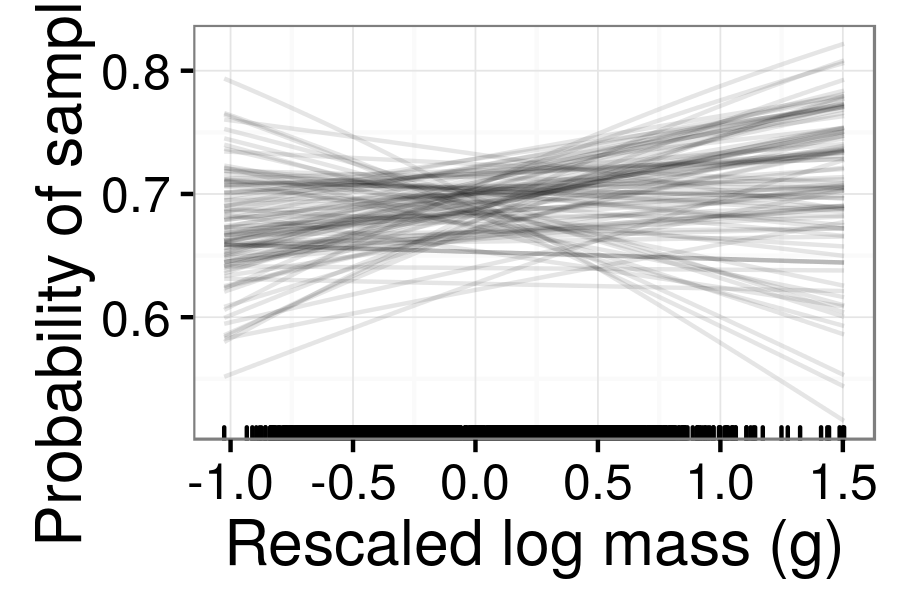
\includegraphics[width=\textwidth,height=0.4\textheight,keepaspectratio=true]{chapter_coping/figure/mass_on_samp}
    \caption{Pure-presence model}
    \label{fig:mass_preserve_pure_pres}
  \end{subfigure}
  \begin{subfigure}[b]{0.45\textwidth}
    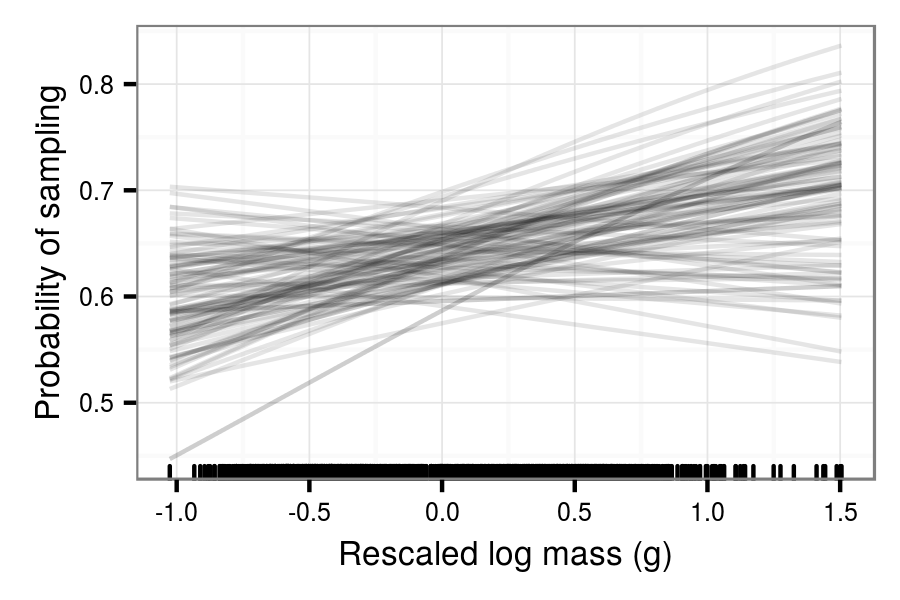
\includegraphics[width=\textwidth,height=0.4\textheight,keepaspectratio=true]{chapter_coping/figure/mass_on_samp_bd}
    \caption{Birth-death model}
    \label{fig:mass_preserve_bd}
  \end{subfigure}
  \caption[Estimates of the effect of mass on observation probability]{Estimates of the effect of species mass on probability of sampling a present species (\(p\)). Mass has been log-transformed, centered, and rescaled; this means that a mass of 0 corresponds to the mean of log-mass of all observed species and that mass is in standard deviation units. Estimates are from both the pure-presence and birth-death models.}
  \label{fig:mass_preserve}
\end{figure}

%For the pure-presence model, species mass is found to have either no relationship with occurrence or a negative one (Fig. \ref{fig:mass_occur}). A negative relationship between body size and occurrence is interpreted to mean that large bodied species are likely to occur less frequently than smaller bodied species. Note that all variation in estimates between ecotypes (Fig. \ref{fig:mass_occur}) is due to differences in ecotype-specific occurrence probability and the associated effects of plant phase; the effect of mass was considered constant for all ecotypes.

There is broad congruence between the estimated effect of body mass on occurrence probability (Fig. \ref{fig:mass_occur}) and the effect of species mass on body mass on origination probability (Fig. \ref{fig:mass_origin}). The striking pattern is higher probability of origination for species with body sizes closer to the mean than either extremes. This result is consistent with the canonically normal distribution of mammal body sizes \citep{Smith2004}; it is then expected that the most likely to occur species would be those from the middle of the distribution, and that species originating will on average be of average mass, especially considering species shared common ancestry \citep{Felsenstein1985b}. All variation in estimates between ecotypes (Fig. \ref{fig:mass_occur}, \ref{fig:mass_origin}) is due to differences in ecotype-specific origination probabilities and the associated effects of plant phase; the effect of mass was considered constant for all ecotypes.

\begin{figure}[ht]
  \centering
  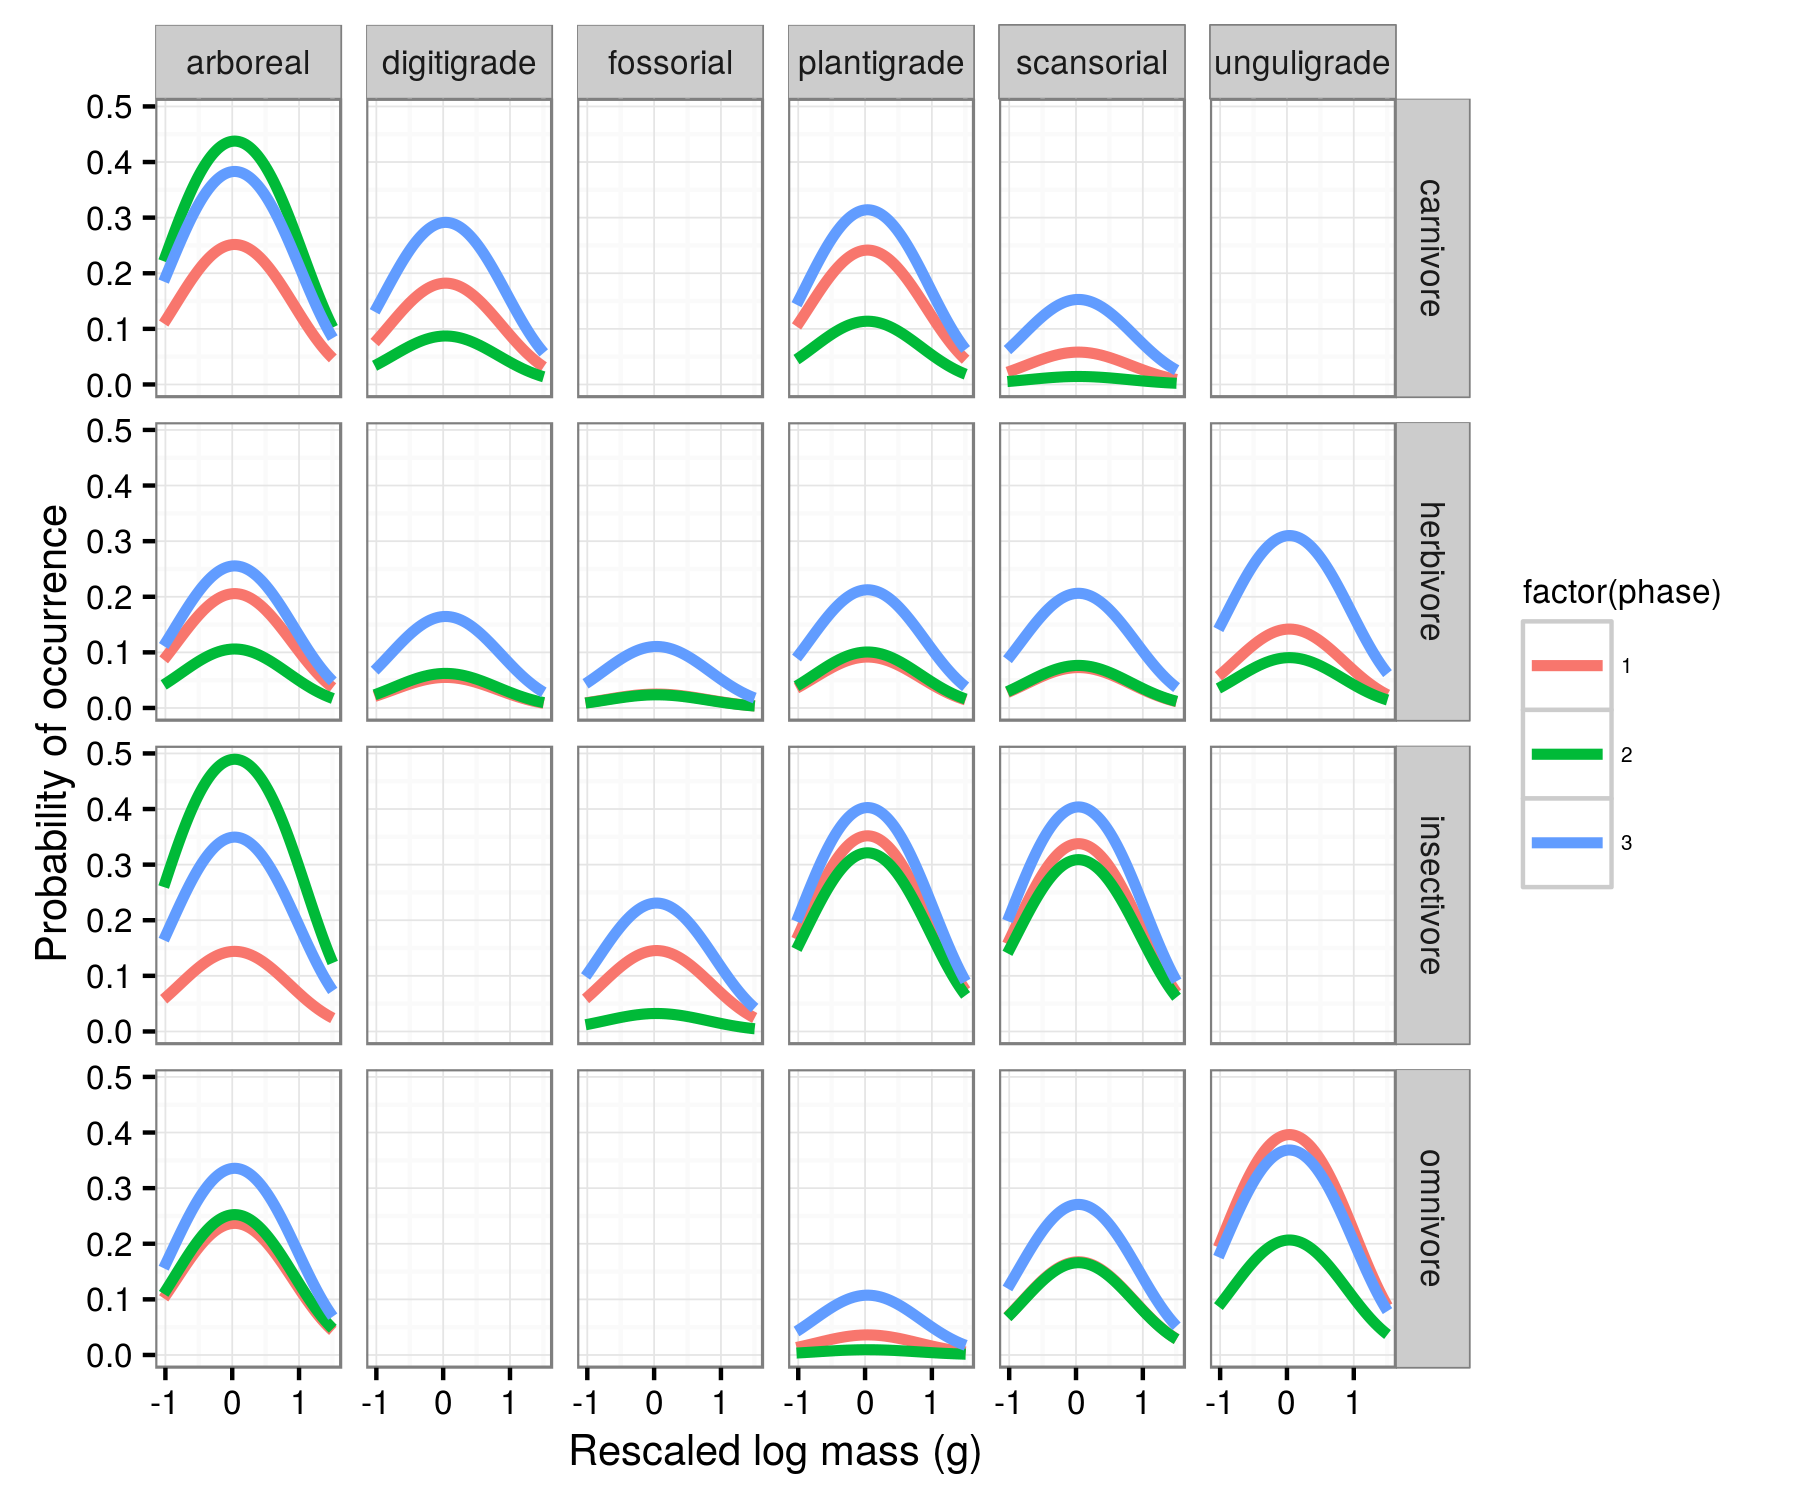
\includegraphics[width=\textwidth,height=0.4\textheight,keepaspectratio=true]{chapter_coping/figure/mass_on_pres}
  \caption[Effect of mass on probability of species occurrence as estimated from the pure-presence model]{Mean estimate of the effect of species mass on the probability of a species occurrence for each of the three plant phases. The effect of mass is considered constant over time and that the only aspect of the model that changes with plant phase is the intercept of the relationship between mass and occurrence. The three plant phases are indicated by the color of the line. Mass has been log-transformed, centered, and rescaled; this means that a mass of 0 corresponds to the mean of log-mass of all observed species and that mass is in standard deviation units. For clarity, only the mean estimates of the effects of mass and plant phase are plotted.}
  \label{fig:mass_occur}
\end{figure}

\begin{figure}[ht]
  \centering
  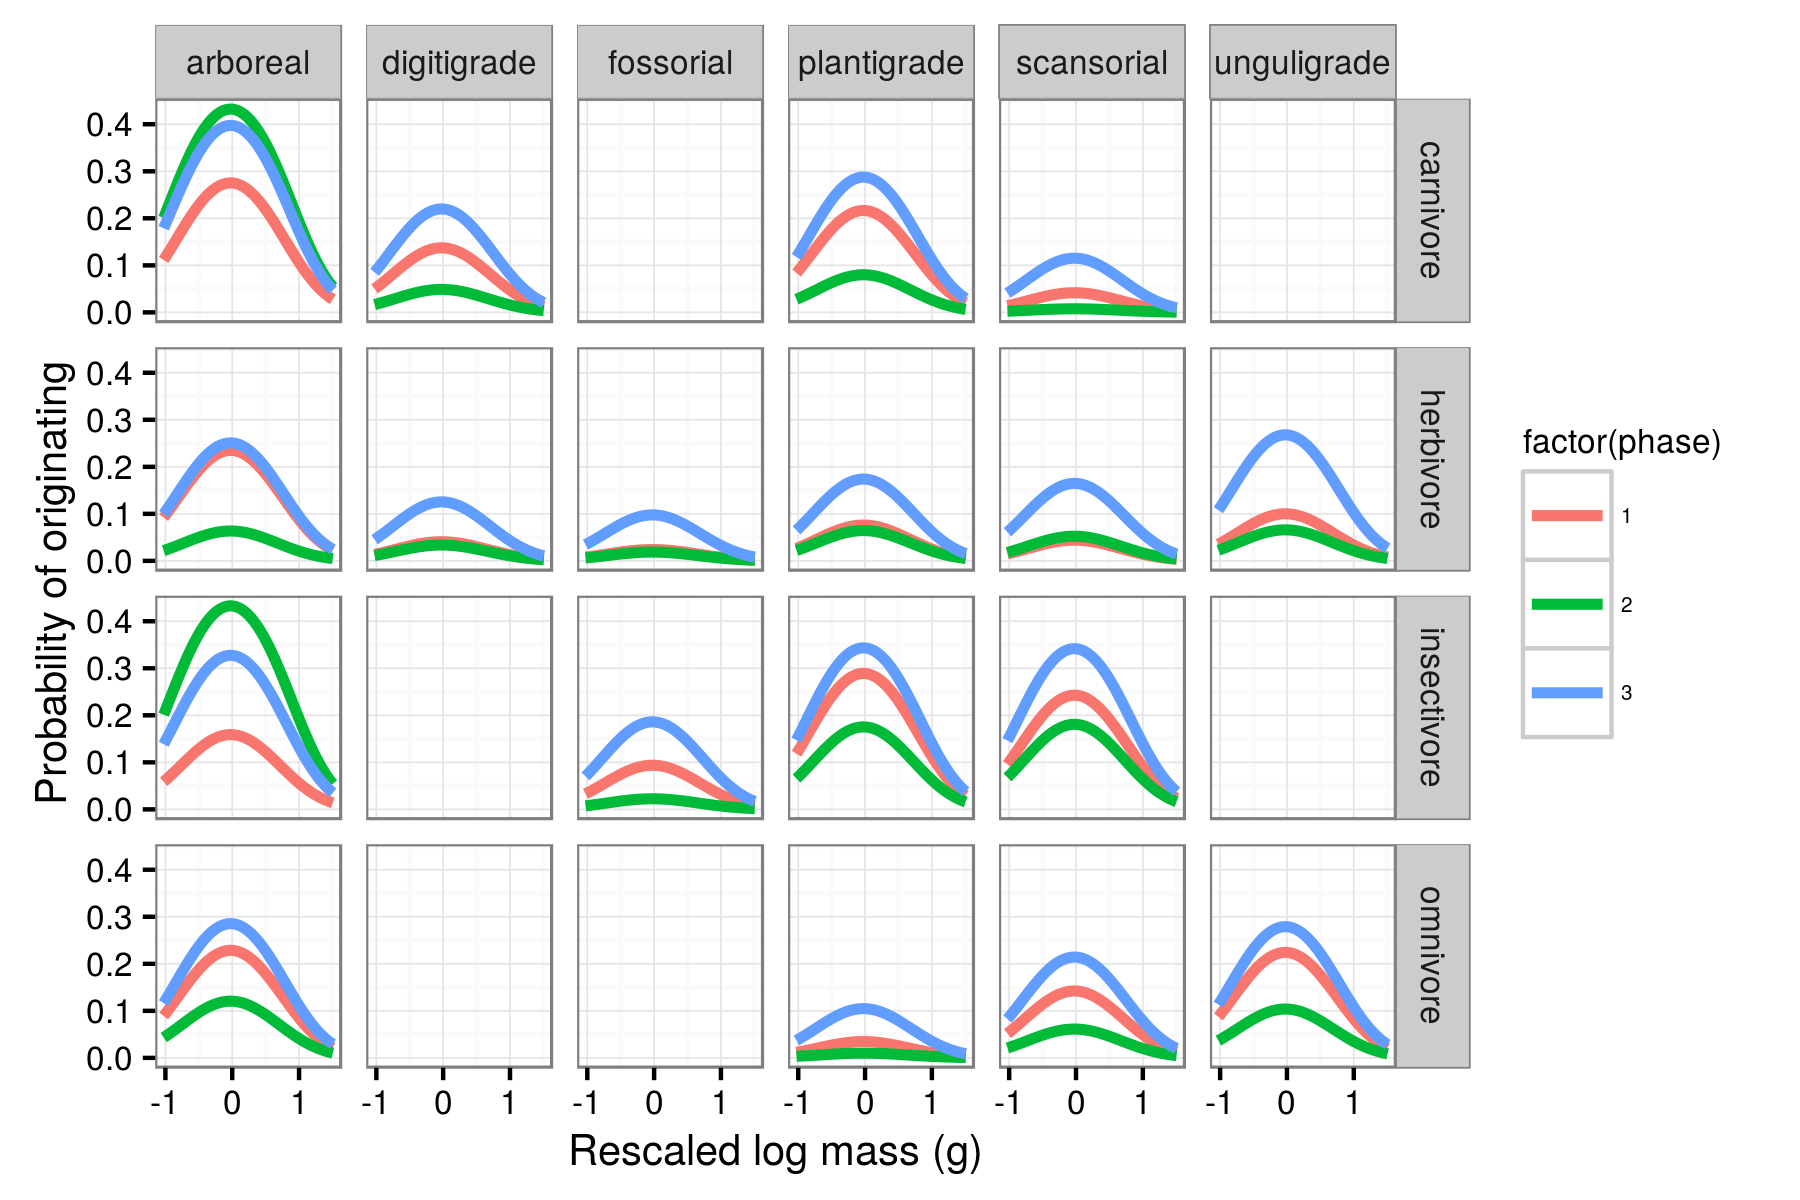
\includegraphics[width=\textwidth,height=0.4\textheight,keepaspectratio=true]{chapter_coping/figure/mass_on_origin_bd}
  \caption[Effect of mass on probability of species origination as estimated from the birth-death model]{Mean estimate of the effect of species mass on the probability of a species originating for each of the three plant phases. The effect of mass is considered constant over time and that the only aspect of the model that changes with plant phase is the intercept of the relationship between mass and origination. The three plant phases are indicated by the color of the line. Mass has been log-transformed, centered, and rescaled; this means that a mass of 0 corresponds to the mean of log-mass of all observed species and that mass is in standard deviation units. For clarity, only the mean estimates of the effects of mass and plant phase are plotted.}
  \label{fig:mass_origin}
\end{figure}

In contrast, the effect of species mass on probability of survival as estimated from the birth-death model (Fig. \ref{fig:mass_survival}) is consistent with previous findings that there is little effect of mass on extinction for North American mammals for the Cenozoic \citep{Smits2015b,Tomiya2013}. Note that all variation between ecotypes depicted in Figure \ref{fig:mass_survival} is due to differences in ecotype-specific survival probability and the associated effects of plant phase; the effect of mass was considered constant for all ecotypes (Eqs. \ref{eq:pure_presence}, \ref{eq:birth_death}).

\begin{figure}[ht]
  \centering
  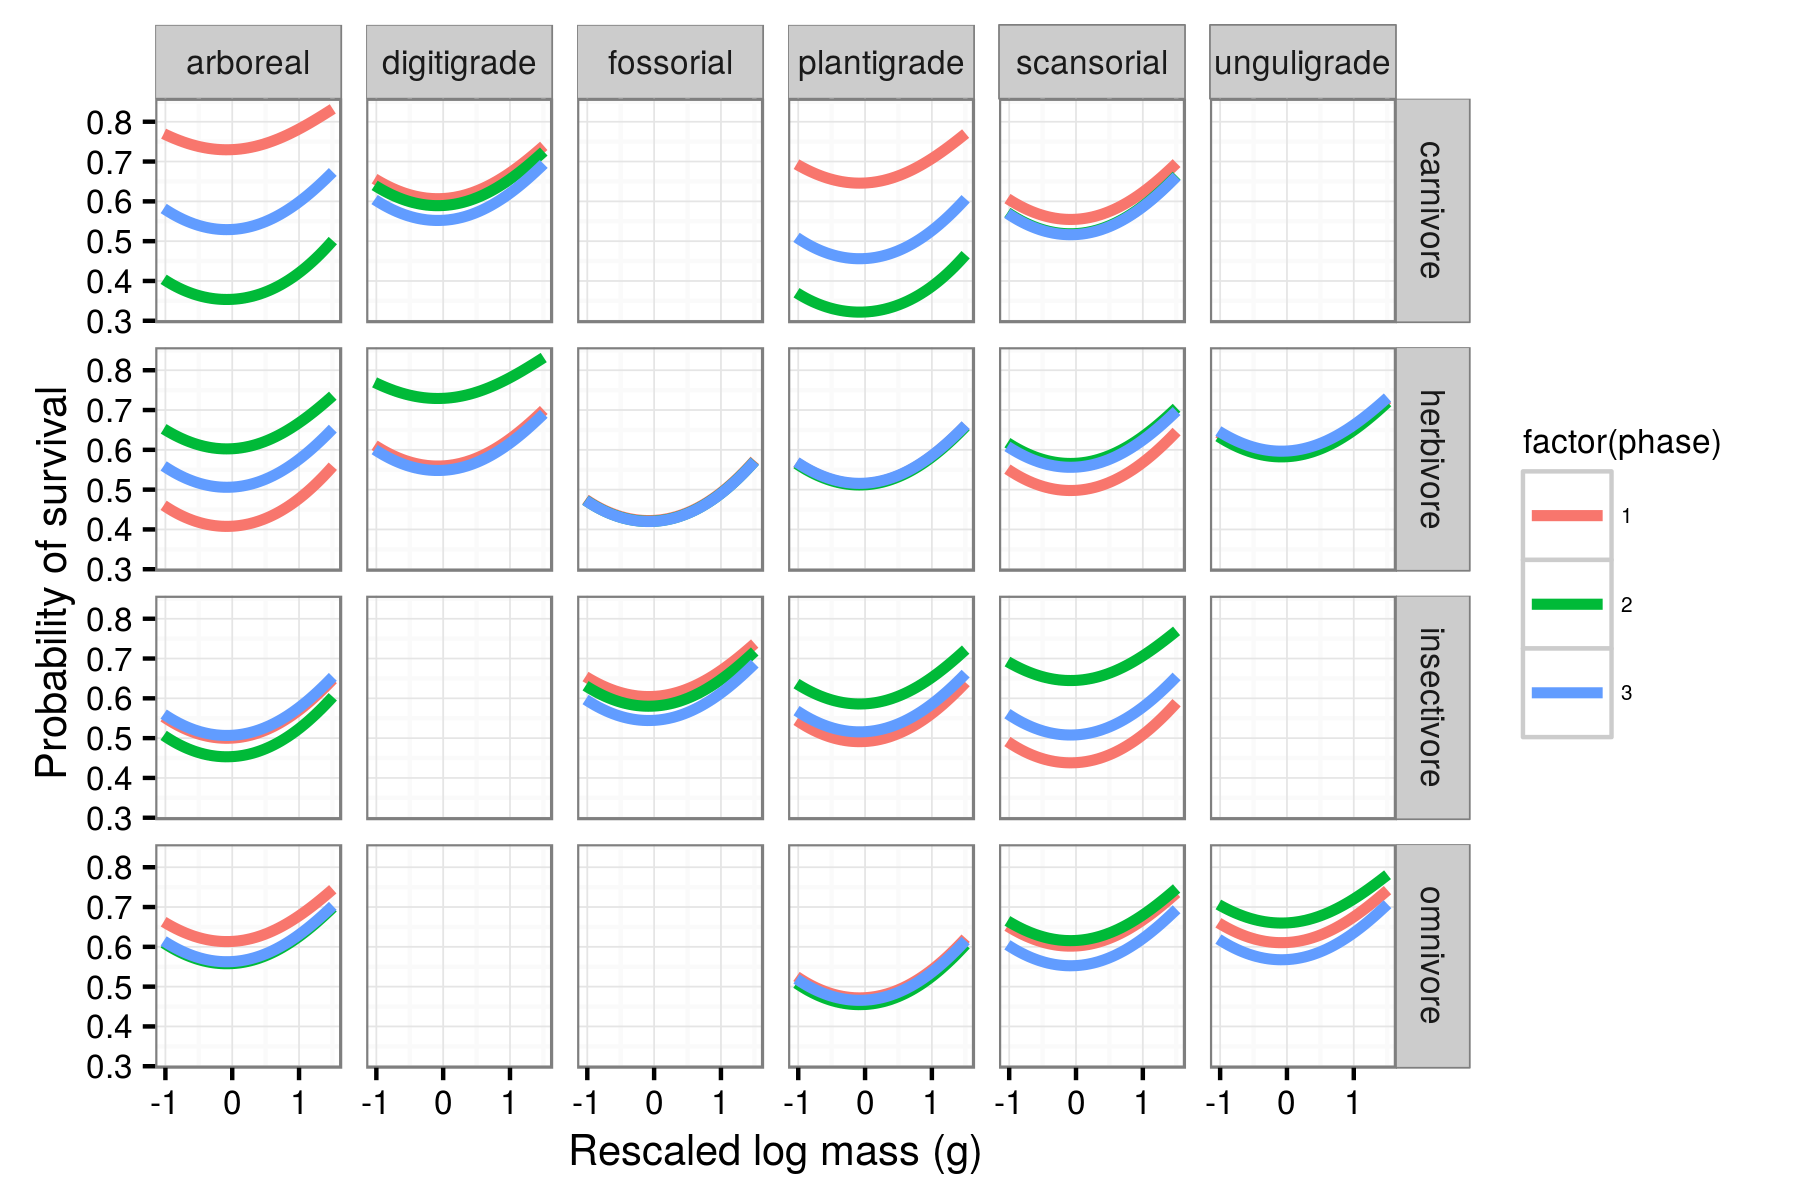
\includegraphics[width=\textwidth,height=0.4\textheight,keepaspectratio=true]{chapter_coping/figure/mass_on_surv_bd}
  \caption[Effect of mass on probability of species survival as estimated from the birth-death model]{Mean estimate of the effect of species mass on the probability of a species survival for each of the three plant phases. The effect of mass is considered constant over time and that the only aspect of the model that changes with plant phase is the intercept of the relationship between mass and survival. The three plant phases are indicated by the color of the line. Mass has been log-transformed, centered, and rescaled; this means that a mass of 0 corresponds to the mean of log-mass of all observed species and that mass is in standard deviation units. For clarity, only the mean estimates of the effects of mass and plant plant are plotted.}
  \label{fig:mass_survival}
\end{figure}


Similarities in parameter estimates between ecotypes may be due to a similar response to environmental factors (Fig. \ref{fig:group_pure_presence}, \ref{fig:group_origin_bd}, and \ref{fig:group_surv_bd}). The estimated group-level effects on ecotype occurrence, origination, or survival are all very different from each other. At best, the effects of temperature on occurrence and origination can be considered congruent (Fig. \ref{fig:group_pure_presence}, \ref{fig:group_origin_bd}). As demonstrated in the comparisons of the effect of body mass on occurrence from the pure-presence model (Fig. \ref{fig:mass_occur}) with the effect of body mass on origination and survival from the birth-death model (Fig. \ref{fig:mass_origin}, and \ref{fig:mass_survival}), there is considerable variation in the effect of plant phases on ecotype-specific estimates.


\begin{figure}[ht]
  \centering
  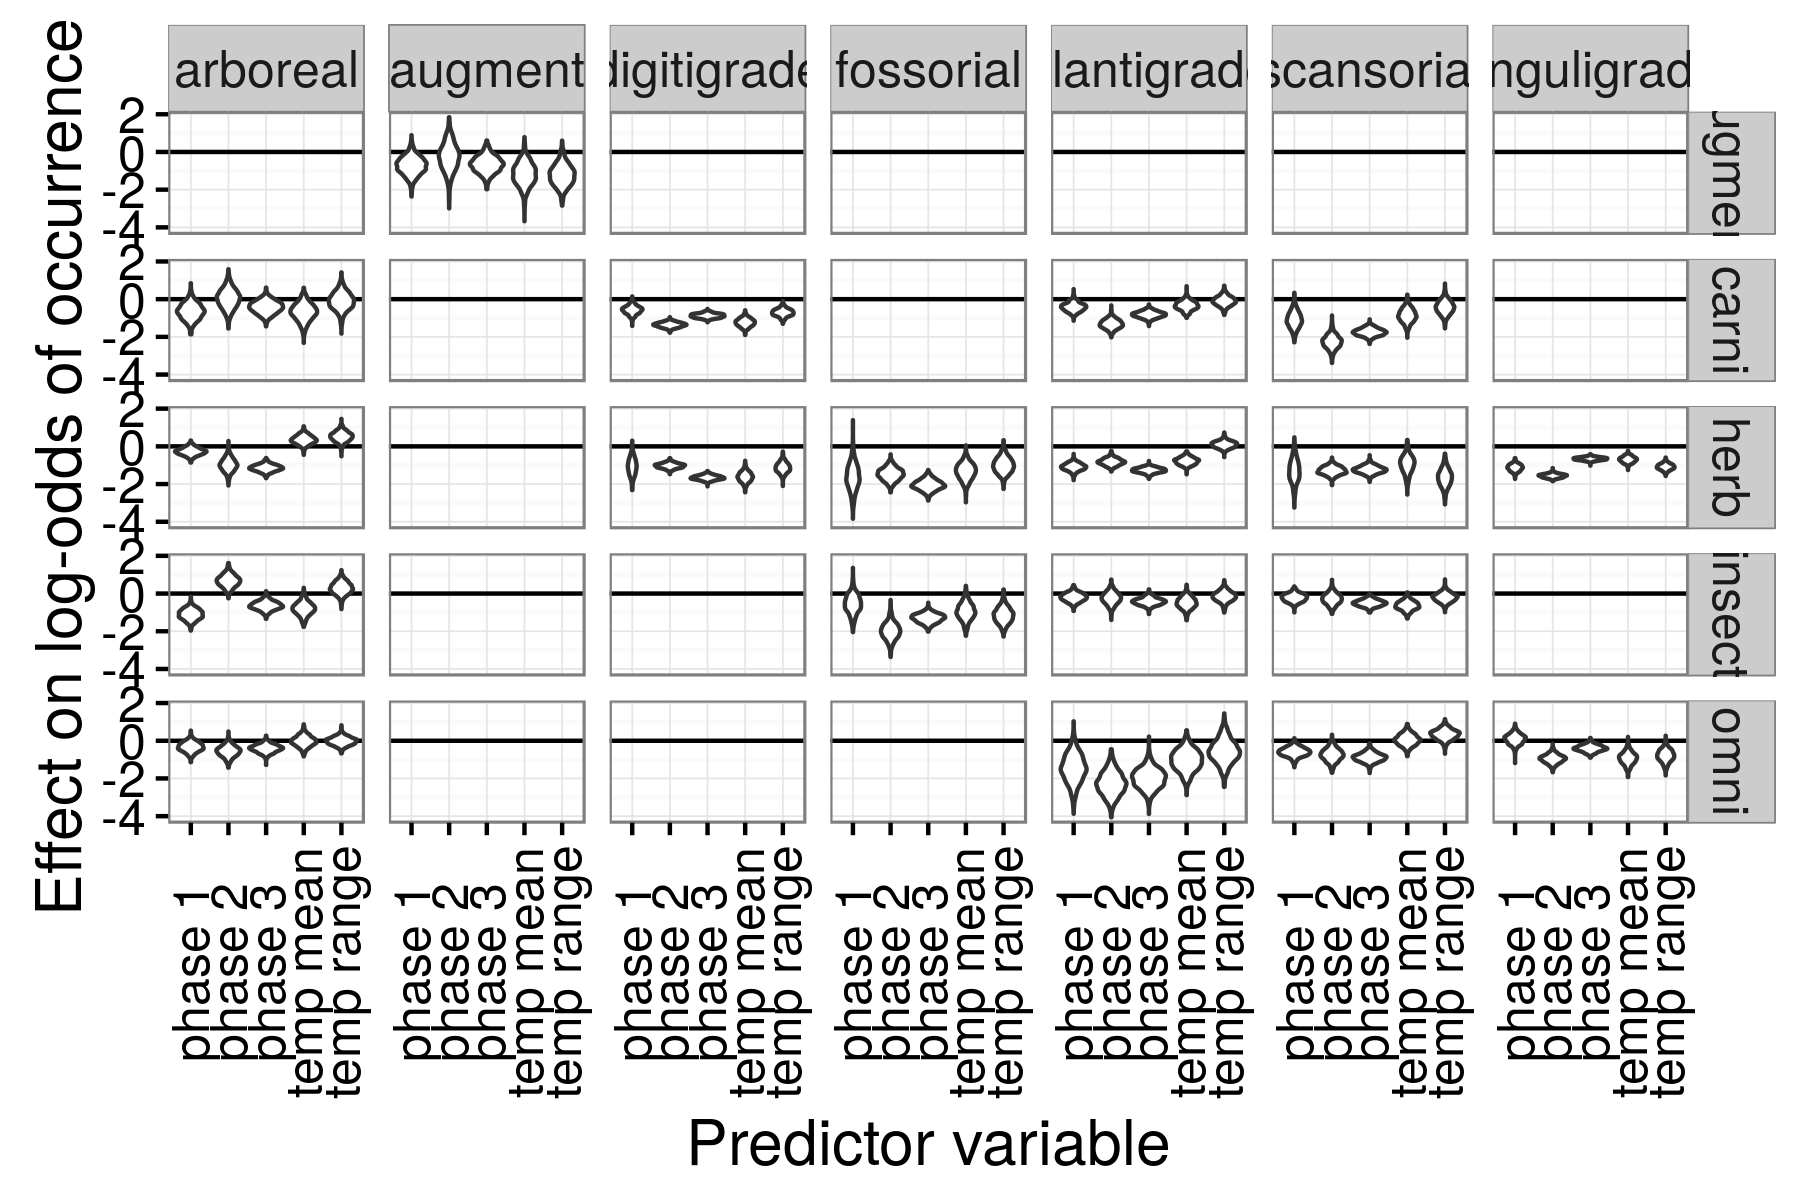
\includegraphics[width=\textwidth,height=0.4\textheight,keepaspectratio=true]{chapter_coping/figure/group_on_ecotype}
  \caption[Effects of group-level covariates on log-odds of ecotype occurrence as estimated from the pure-presence model]{Estimated effects of the group-level covariates describing environmental context on log-odds of species occurrence. These estimates are from the pure-presence model. What is plotted is a violin of the distribution of 1000 samples from the approximate posterior. The effect of plant phase graphed here is calculated as Phase 1\( = \gamma_{phase\ 1}\), Phase 2\( = \gamma_{phase\ 1} + \gamma_{phase\ 2}\), and so on.} 
  \label{fig:group_pure_presence}
\end{figure}

\begin{figure}[ht]
  \centering
  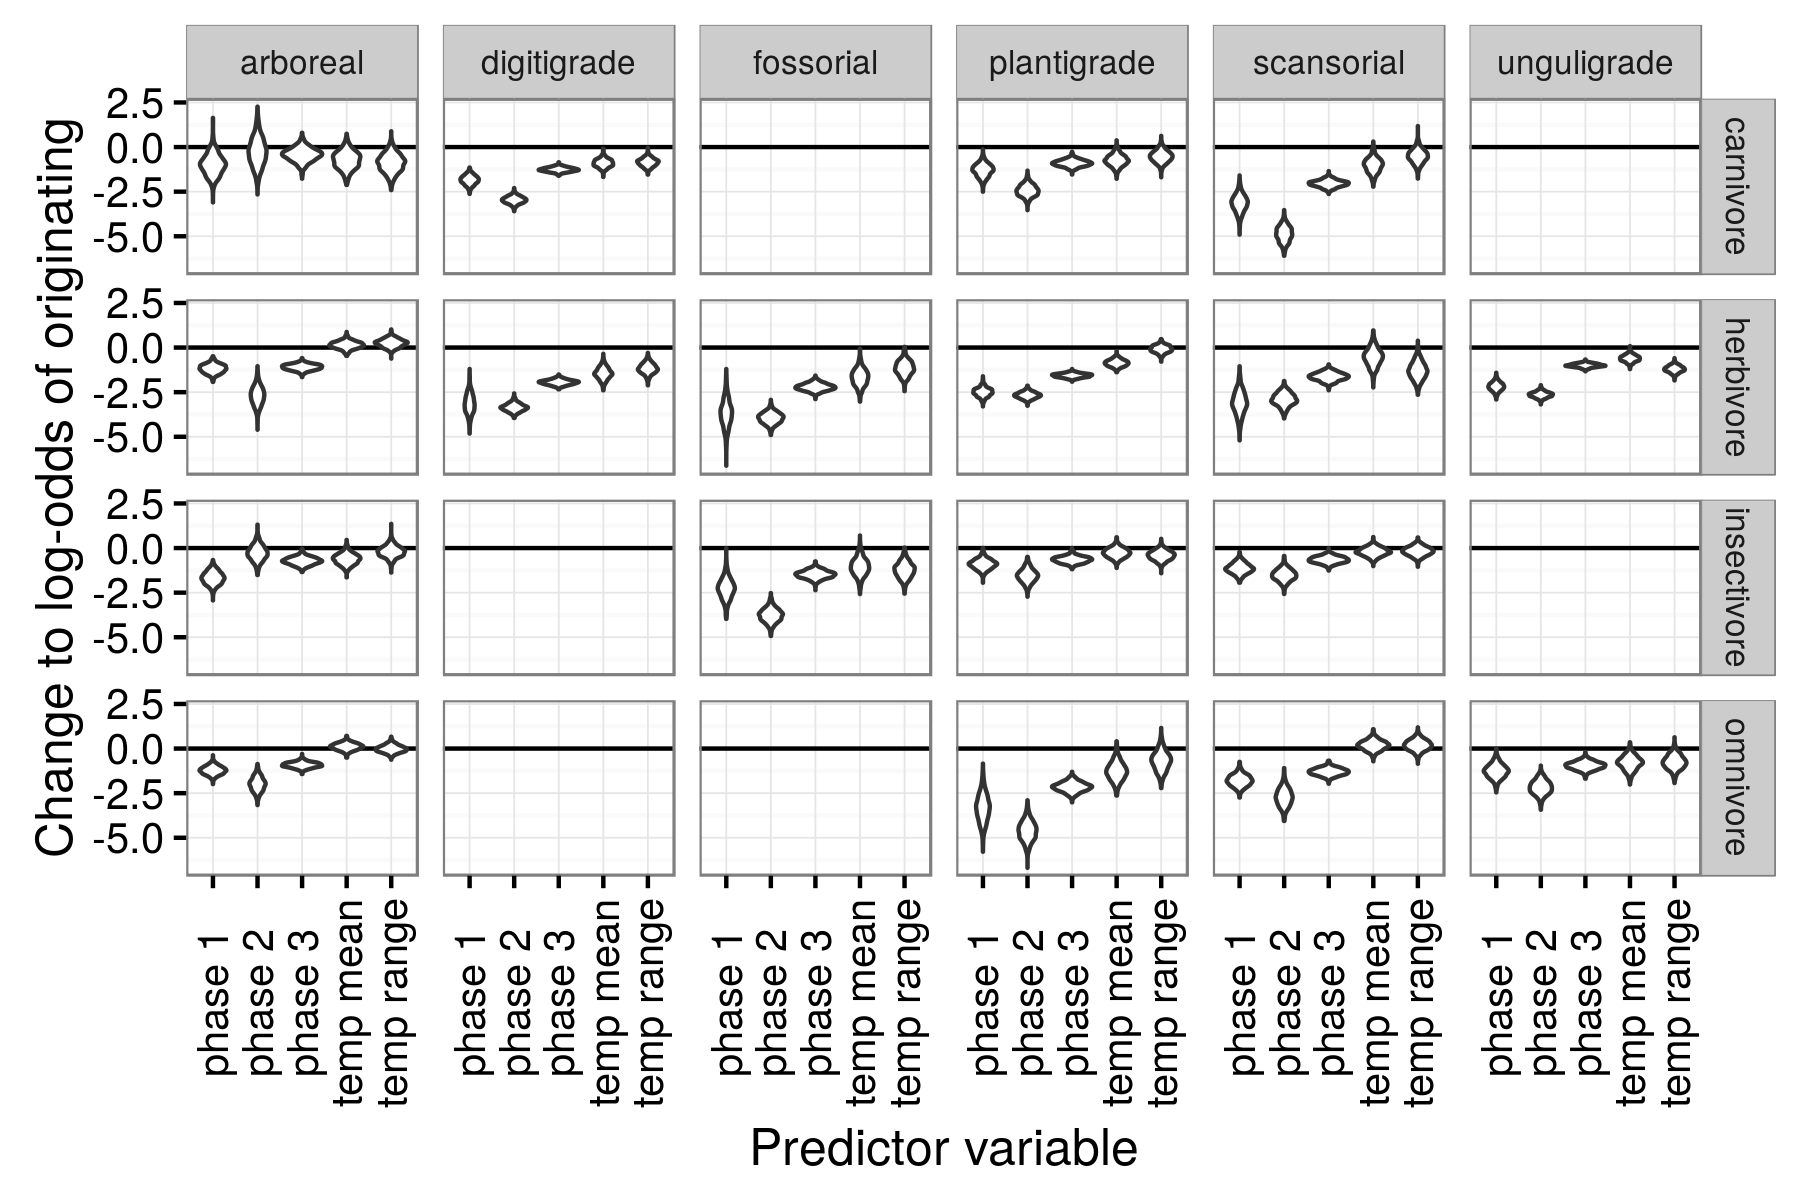
\includegraphics[width=\textwidth,height=0.4\textheight,keepaspectratio=true]{chapter_coping/figure/group_on_origin_bd}
  \caption[Effects of group-level covariates on log-odds of ecotype origination as estimated from the birth-death model]{Estimated effects of the group-level covariates describing environmental context on log-odds of species origination. These estimates are from the birth-death model. What is plotted is a violin of the distribution of 1000 samples from the approximate posterior. The effect of plant phase graphed here is calculated as Phase 1\( = \gamma_{phase\ 1}\), Phase 2\( = \gamma_{phase\ 1} + \gamma_{phase\ 2}\), and so on.} 
  \label{fig:group_origin_bd}
\end{figure}

\begin{figure}[ht]
  \centering
  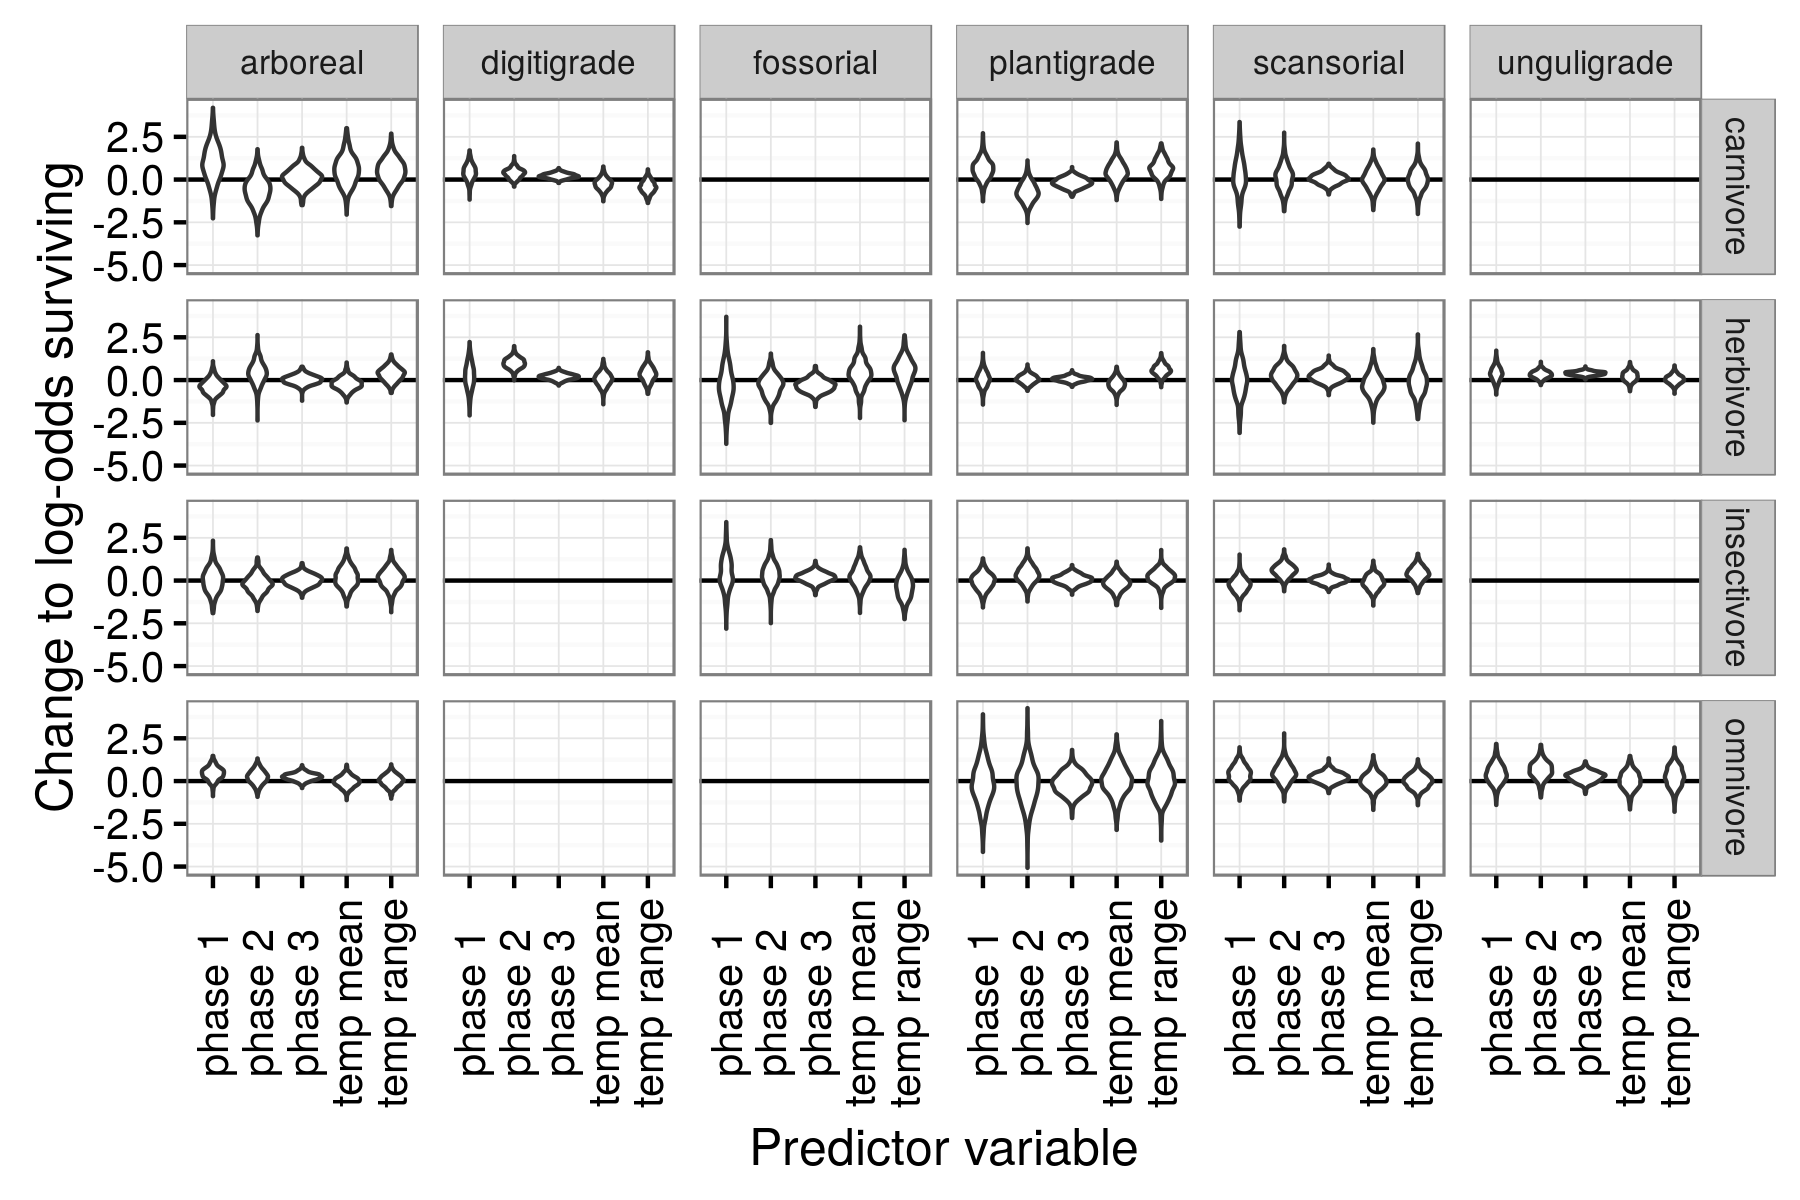
\includegraphics[width=\textwidth,height=0.4\textheight,keepaspectratio=true]{chapter_coping/figure/group_on_survival_bd}
  \caption[Effects of group-level covariates on log-odds of ecotype survival as estimated from the birth-death model]{Estimated effects of the group-level covariates describing environmental context on log-odds of species survival. These estimates are from the birth-death model. What is plotted is a violin of the distribution of 1000 samples from the approximate posterior. The effect of plant phase graphed here is calculated as Phase 1\( = \gamma_{phase\ 1}\), Phase 2\( = \gamma_{phase\ 1} + \gamma_{phase\ 2}\), and so on.} 
  \label{fig:group_surv_bd}
\end{figure}



An association between plant phase and differences in the log-odds of occurrence (Fig. \ref{fig:group_pure_presence}), origination (Fig. \ref{fig:group_origin_bd}), or extinction (Fig. \ref{fig:group_surv_bd}) is interpreted to mean that the set of possible mammal-plant interactions was relatively more favorable (positive association) or less so (negative association) to those ecotypes. In the case of species origination, for example, more favorable conditions for an ecotype may indicate an increasing number of possible and available mammal-plant interactions (e.g. ecological opportunity; \citealp{Yoder2010,Losos2010,Losos2010a}); while adverse conditions may translate to a decreasing set of interactions or loss of appropriate environmental context. Remember that favorable versus adverse condition of a plant phase is definitionally relative to the other two plant phases. 

One of the limitations to this interpretation is the almost determistic increase in probability of occurrence and origination for most ecotypes (Fig. \ref{fig:eco_occur}, \ref{fig:eco_origin}). This ``pull of the Recent'' means that interpreting the biological meaning of differences between the final plant phase and the two previous phases is difficult as the guanteed occurrence of the later taxa increases the average probability for that phase, which in turn affects the other time bins in that phase.

Plant phases are associated with large differences in log-odds for occurrence and origination probabilities (Tables \ref{tab:occur_plant}, \ref{tab:origin_plant}), though there is little evidence of plant phase being an important distinguishing factor in species survival, as only a few ecotypes demonstrate strong affinities with some plant phases (Table \ref{tab:surv_plant}). 

The effects of plant phase on occurrence and origination probabilities are broadly congruent with each other (Fig. \ref{fig:group_pure_presence}, \ref{fig:group_origin_bd}). The almost universal pattern of the effect of plant phase on ecotype origination is that the during first and last plant phases ecotypes have a greater log-odds of occurrence or origination than the second plant phase (Fig. \ref{fig:eco_occur}, \ref{fig:eco_origin}). The three ecotypes that do not follow this pattern are fossorial herbivores, scansorial herbivores, and arboreal insectivores.


\begin{table}[ht]
  \centering
  \caption[Posterior probablity estimates of differences in occurrence by plant phase]{Posterior probability of the differences in the log-odds of an ecotype occurring based on plant phase. These probabilities are calculated as P(Phase 1 \(>\) 2) = \( (\sum \gamma_{phase 1} > \gamma_{phase 1} + \gamma_{phase 2}) / 100\) and similarly for the other comparisons. These estimates are from the pure-presence model.}
  \label{tab:occur_plant}
  \begin{tabular}{ l r r r }
    \hline
    & P(Phase 1 $>$ Phase 2) & P(Phase 2 $>$ Phase 3) & P(Phase 1 $>$ Phase 3) \\ 
    \hline
    arboreal carnivore & 0.323 & 0.874 & 0.926 \\ 
    digitigrade carnivore & 1.000 & 0.000 & 1.000 \\ 
    plantigrade carnivore & 1.000 & 0.040 & 1.000 \\ 
    scansorial carnivore & 1.000 & 0.015 & 1.000 \\ 
    arboreal herbivore & 1.000 & 0.515 & 1.000 \\ 
    digitigrade herbivore & 1.000 & 0.995 & 1.000 \\ 
    fossorial herbivore & 1.000 & 0.923 & 1.000 \\ 
    plantigrade herbivore & 1.000 & 0.995 & 1.000 \\ 
    scansorial herbivore & 1.000 & 0.717 & 1.000 \\ 
    unguligrade herbivore & 1.000 & 0.000 & 1.000 \\ 
    arboreal insectivore & 0.024 & 0.999 & 0.997 \\ 
    fossorial insectivore & 1.000 & 0.000 & 1.000 \\ 
    plantigrade insectivore & 0.923 & 0.558 & 0.985 \\ 
    scansorial insectivore & 0.982 & 0.483 & 0.992 \\ 
    arboreal omnivore & 0.959 & 0.837 & 1.000 \\ 
    plantigrade omnivore & 1.000 & 0.247 & 1.000 \\ 
    scansorial omnivore & 0.983 & 0.861 & 1.000 \\ 
    unguligrade omnivore & 1.000 & 0.189 & 0.998 \\ 
    \hline
  \end{tabular}
\end{table}

\begin{table}[ht]
  \centering
  \caption[Posterior probablity estimates of differences in origination by plant phase]{Posterior probability of the differences in the log-odds of an ecotype originating based on plant phase. These probabilities are calculated as P(Phase 1 \(>\) 2) = \( (\sum \gamma_{phase 1} > \gamma_{phase 1} + \gamma_{phase 2}) / 100\) and similarly for the other comparisons. These estimates are from the birth-death model.}
  \label{tab:origin_plant}
  \begin{tabular}{ l r r r }
    \hline
    & P(Phase 1 $>$ Phase 2) & P(Phase 2 $>$ Phase 3) & P(Phase 1 $>$ Phase 3) \\ 
    \hline
    arboreal carnivore & 0.405 & 0.777 & 0.905 \\ 
    digitigrade carnivore & 1.000 & 0.043 & 1.000 \\ 
    plantigrade carnivore & 1.000 & 0.053 & 1.000 \\ 
    scansorial carnivore & 1.000 & 0.035 & 1.000 \\ 
    arboreal herbivore & 1.000 & 0.163 & 1.000 \\ 
    digitigrade herbivore & 1.000 & 0.998 & 1.000 \\ 
    fossorial herbivore & 1.000 & 0.896 & 1.000 \\ 
    plantigrade herbivore & 1.000 & 0.996 & 1.000 \\ 
    scansorial herbivore & 1.000 & 0.884 & 1.000 \\ 
    unguligrade herbivore & 1.000 & 0.003 & 1.000 \\ 
    arboreal insectivore & 0.088 & 0.994 & 1.000 \\ 
    fossorial insectivore & 1.000 & 0.020 & 1.000 \\ 
    plantigrade insectivore & 0.995 & 0.419 & 1.000 \\ 
    scansorial insectivore & 0.999 & 0.360 & 1.000 \\ 
    arboreal omnivore & 0.999 & 0.317 & 1.000 \\ 
    plantigrade omnivore & 1.000 & 0.308 & 1.000 \\ 
    scansorial omnivore & 0.999 & 0.418 & 1.000 \\ 
    unguligrade omnivore & 1.000 & 0.219 & 1.000 \\ 
    \hline
  \end{tabular}
\end{table}


\begin{table}[ht]
  \centering
  \caption[Posterior probablity estimates of differences in survival by plant phase]{Posterior probability of the differences in the log-odds of an ecotype surviving based on plant phase. These probabilities are calculated as P(Phase 1 \(>\) 2) = \( (\sum \gamma_{phase 1} > \gamma_{phase 1} + \gamma_{phase 2}) / 100\) and similarly for the other comparisons. These estimates are from the birth-death model.}
  \label{tab:surv_plant}
  \begin{tabular}{ l r r r }
    \hline
    & P(Phase 1 $>$ Phase 2) & P(Phase 2 $>$ Phase 3) & P(Phase 1 $>$ Phase 3) \\ 
    \hline
    arboreal carnivore & 0.849 & 0.127 & 0.313 \\ 
    digitigrade carnivore & 0.292 & 0.411 & 0.162 \\ 
    plantigrade carnivore & 0.926 & 0.243 & 0.790 \\ 
    scansorial carnivore & 0.409 & 0.544 & 0.453 \\ 
    arboreal herbivore & 0.250 & 0.733 & 0.480 \\ 
    digitigrade herbivore & 0.000 & 0.990 & 0.246 \\ 
    fossorial herbivore & 0.547 & 0.680 & 0.812 \\ 
    plantigrade herbivore & 0.404 & 0.555 & 0.480 \\ 
    scansorial herbivore & 0.534 & 0.277 & 0.204 \\ 
    unguligrade herbivore & 0.600 & 0.046 & 0.003 \\ 
    arboreal insectivore & 0.673 & 0.379 & 0.539 \\ 
    fossorial insectivore & 0.464 & 0.442 & 0.308 \\ 
    plantigrade insectivore & 0.216 & 0.714 & 0.446 \\ 
    scansorial insectivore & 0.019 & 0.923 & 0.382 \\ 
    arboreal omnivore & 0.394 & 0.440 & 0.242 \\ 
    plantigrade omnivore & 0.582 & 0.542 & 0.677 \\ 
    scansorial omnivore & 0.292 & 0.590 & 0.289 \\ 
    unguligrade omnivore & 0.212 & 0.555 & 0.183 \\ 
    \hline
  \end{tabular}
\end{table}


Both aspects of global temperature analyzed here are estimated to have strong effects on species occurrence and origination for most mammal ecotypes (Tables \ref{tab:occur_temp}, \ref{tab:origin_temp}). Similarly, the probability that temperature has a large effect on species extinction is very low for all ecotypes (Table \ref{tab:surv_temp}). The effects of the temperature covariates on ecotype occurrence and origination are estimated to be negative, which which means that as temperature decreases, occurrence and origination are expected to increase. In the case of survival, the only strong ecotype association for either of the temperature covariates is a positive relationship between temperature range and occurrence probabilities of with plantigrade herbivores (Tab. \ref{tab:surv_temp}).

\begin{table}[ht]
  \centering
  \caption[Posterior probablity of effects of temperature on occurrence]{Posterior probabilities that the effects of the two temperature covariates on the log-odds of an ecotype occurring are greater than 0. What is estimated is the probability that these estimates are greater than 0; high or low probabilities indicate the ``strength'' of the covariate in that direction (positive and negative, respectively). These estimates are from the pure-presence model.}
  \label{tab:occur_temp}
  \begin{tabular}{ l r r }
    \hline
    & \(P(\gamma_{temp\ mean} > 0)\) & \(P(\gamma_{temp\ range} > 0)\) \\ 
    \hline
    arboreal carnivore & 0.067 & 0.043 \\ 
    digitigrade carnivore & 0.000 & 0.000 \\ 
    plantigrade carnivore & 0.012 & 0.054 \\ 
    scansorial carnivore & 0.007 & 0.086 \\ 
    arboreal herbivore & 0.762 & 0.852 \\ 
    digitigrade herbivore & 0.000 & 0.000 \\ 
    fossorial herbivore & 0.000 & 0.002 \\ 
    plantigrade herbivore & 0.000 & 0.364 \\ 
    scansorial herbivore & 0.141 & 0.004 \\ 
    unguligrade herbivore & 0.001 & 0.000 \\ 
    arboreal insectivore & 0.031 & 0.251 \\ 
    fossorial insectivore & 0.014 & 0.002 \\ 
    plantigrade insectivore & 0.164 & 0.058 \\ 
    scansorial insectivore & 0.197 & 0.250 \\ 
    arboreal omnivore & 0.711 & 0.449 \\ 
    plantigrade omnivore & 0.009 & 0.103 \\ 
    scansorial omnivore & 0.754 & 0.732 \\ 
    unguligrade omnivore & 0.015 & 0.022 \\ 
    \hline
  \end{tabular}
\end{table}



\begin{table}[ht]
  \centering
  \caption[Posterior probablity of effects of temperature on origination]{Posterior probability that the effects of the two temperature covariates on the log-odds of an ecotype origination are greater than 0. What is estimated is the probability that these estimates are greater than 0; high or low probabilities indicate the ``strength'' of the covariate in that direction (positive and negative, respectively). These estimates are from the birth-death model.}
  \label{tab:origin_temp}
  \begin{tabular}{ l r r }
    \hline
    & \(P(\gamma_{temp\ mean} > 0)\) & \(P(\gamma_{temp\ range} > 0)\) \\ 
    \hline
    arboreal carnivore & 0.072 & 0.031 \\ 
    digitigrade carnivore & 0.000 & 0.001 \\ 
    plantigrade carnivore & 0.010 & 0.094 \\ 
    scansorial carnivore & 0.006 & 0.104 \\ 
    arboreal herbivore & 0.785 & 0.881 \\ 
    digitigrade herbivore & 0.000 & 0.000 \\ 
    fossorial herbivore & 0.001 & 0.007 \\ 
    plantigrade herbivore & 0.000 & 0.626 \\ 
    scansorial herbivore & 0.097 & 0.002 \\ 
    unguligrade herbivore & 0.010 & 0.000 \\ 
    arboreal insectivore & 0.018 & 0.319 \\ 
    fossorial insectivore & 0.008 & 0.003 \\ 
    plantigrade insectivore & 0.223 & 0.084 \\ 
    scansorial insectivore & 0.139 & 0.202 \\ 
    arboreal omnivore & 0.646 & 0.628 \\ 
    plantigrade omnivore & 0.013 & 0.120 \\ 
    scansorial omnivore & 0.688 & 0.735 \\ 
    unguligrade omnivore & 0.016 & 0.027 \\ 
    \hline
  \end{tabular}
\end{table}

\begin{table}[ht]
  \centering
  \caption[Posterior probablity of effects of temperature on survival]{Posterior probability that the effects of the two temperature covariates on the log-odds of an ecotype survival are greater than 0. What is estimated is the probability that these estimates are greater than 0; high or low probabilities indicate the ``strength'' of the covariate in that direction (positive and negative, respectively). These estimates are from the birth-death model.}
  \label{tab:surv_temp}
  \begin{tabular}{ l r r }
    \hline
    & \(P(\gamma_{temp\ mean} > 0)\) & \(P(\gamma_{temp\ range} > 0)\) \\ 
    \hline
    arboreal carnivore & 0.751 & 0.752 \\ 
    digitigrade carnivore & 0.161 & 0.110 \\ 
    plantigrade carnivore & 0.851 & 0.878 \\ 
    scansorial carnivore & 0.598 & 0.510 \\ 
    arboreal herbivore & 0.281 & 0.819 \\ 
    digitigrade herbivore & 0.546 & 0.721 \\ 
    fossorial herbivore & 0.751 & 0.766 \\ 
    plantigrade herbivore & 0.316 & 0.960 \\ 
    scansorial herbivore & 0.342 & 0.429 \\ 
    unguligrade herbivore & 0.750 & 0.418 \\ 
    arboreal insectivore & 0.572 & 0.579 \\ 
    fossorial insectivore & 0.648 & 0.279 \\ 
    plantigrade insectivore & 0.477 & 0.786 \\ 
    scansorial insectivore & 0.303 & 0.845 \\ 
    arboreal omnivore & 0.536 & 0.611 \\ 
    plantigrade omnivore & 0.499 & 0.507 \\ 
    scansorial omnivore & 0.544 & 0.488 \\ 
    unguligrade omnivore & 0.520 & 0.688 \\ 
    \hline
  \end{tabular}
\end{table}





The apparent similarities in origination rate of digitigrade carnivores, digitigrade herbivores, plantigrade herbivores, and unguligrade herbivores (Fig. \ref{fig:eco_origin} can be tested by inspecting the estimates of the two correlation matrices \(\Omega^{\phi}\) and \(\Omega^{\pi}\). The elements of these matrices are estimates of the correlation in origination and survival probabilities, respectively, between each of the 18 observed ecotypes. However, because ADVI-based inference assumes that the joint posterior is Gaussian, estimates of scale and correlation parameters are very approximate as these parameters tend to have decidedly non-Gaussian true posterior distributions \citep{Gelman2013d}. Because of this fundamental limitation, inference based on these correlation matrices are very approximate and subject to change.

Consistent with visual inspection of the ecotype origination probability time series, there are some strong positive correlations between a few ecotypes (Fig. \ref{fig:origin_corr}). Given the posterior distribution of correlation estimates, the probability of these correlation estimates being greater than 0 can be estimated. Again, because of the assumed Gaussian posterior, these probability estimates are at best approximate and are subject to change given full posterior inference. To visualize these results, I've plotted an association graph of the correlations between ecotypes that are estimated to have a greater than 95\% posterior probability of being greater than 0 (Fig. \ref{fig:origin_corr_graph}); in total there are 35 correlations that fit this criterion. The ecotypes correlated with the most number of other ecotyes, in order from most to least, are unguligrade herbivores, plantigrade herbivores, digitigrade carnivores, scansorial carnivores, fossorial herbivores, and plantigrade omnivores. These results support the conclusion that the origination probabilities of many ecotypes are correlated which I interpret to mean that changes to the species pool's environment context can lead to the simultaneous enrichment of multiple ecotypes instead of each ecotype respondingly independently. This result is most obvious for digitigrade carnivores, scansorial carnivores, digitigrade herbivores, fossorial herbivores, plantigrade herbivores, and unguligrade herbivores; these ecotypes are heavily cross-correlated with each other.

In contrast to the visually obvious correlations in ecotype origination probability, visual inspection of the ecotype-specific survival probabilities (Fig. \ref{fig:eco_survival}) does not indicate that many strong correlations between ecotype survival probabilities. This conclusion is supported by the estimated correlations in ecotype survival probability (Fig. \ref{fig:survival_corr}). There are very few large magnitude estimates of correlation between any of the ecotypes. This result is further supported by the fact that only a single correlation, survival probability of digitigrade carnivores and unguligrade herbivores, has a greater than 95\% posterior probability of being positive (Fig. \ref{fig:surv_corr_graph}). This single correlation, however, adds more nuance to the interpretations from the origination probability correlations. In addition to correlation in enrichment, these ecotypes are correlated in their depletions. This result supports the conclusion that the diversity histories of digitigrade carnivores and unguligrade herbivores are strongly related to each other both in terms of origination and survival, which stands in contrast to those ecotypes which are only correlated for origination.

\afterpage{\clearpage}
\begin{figure}[p]
  \centering
  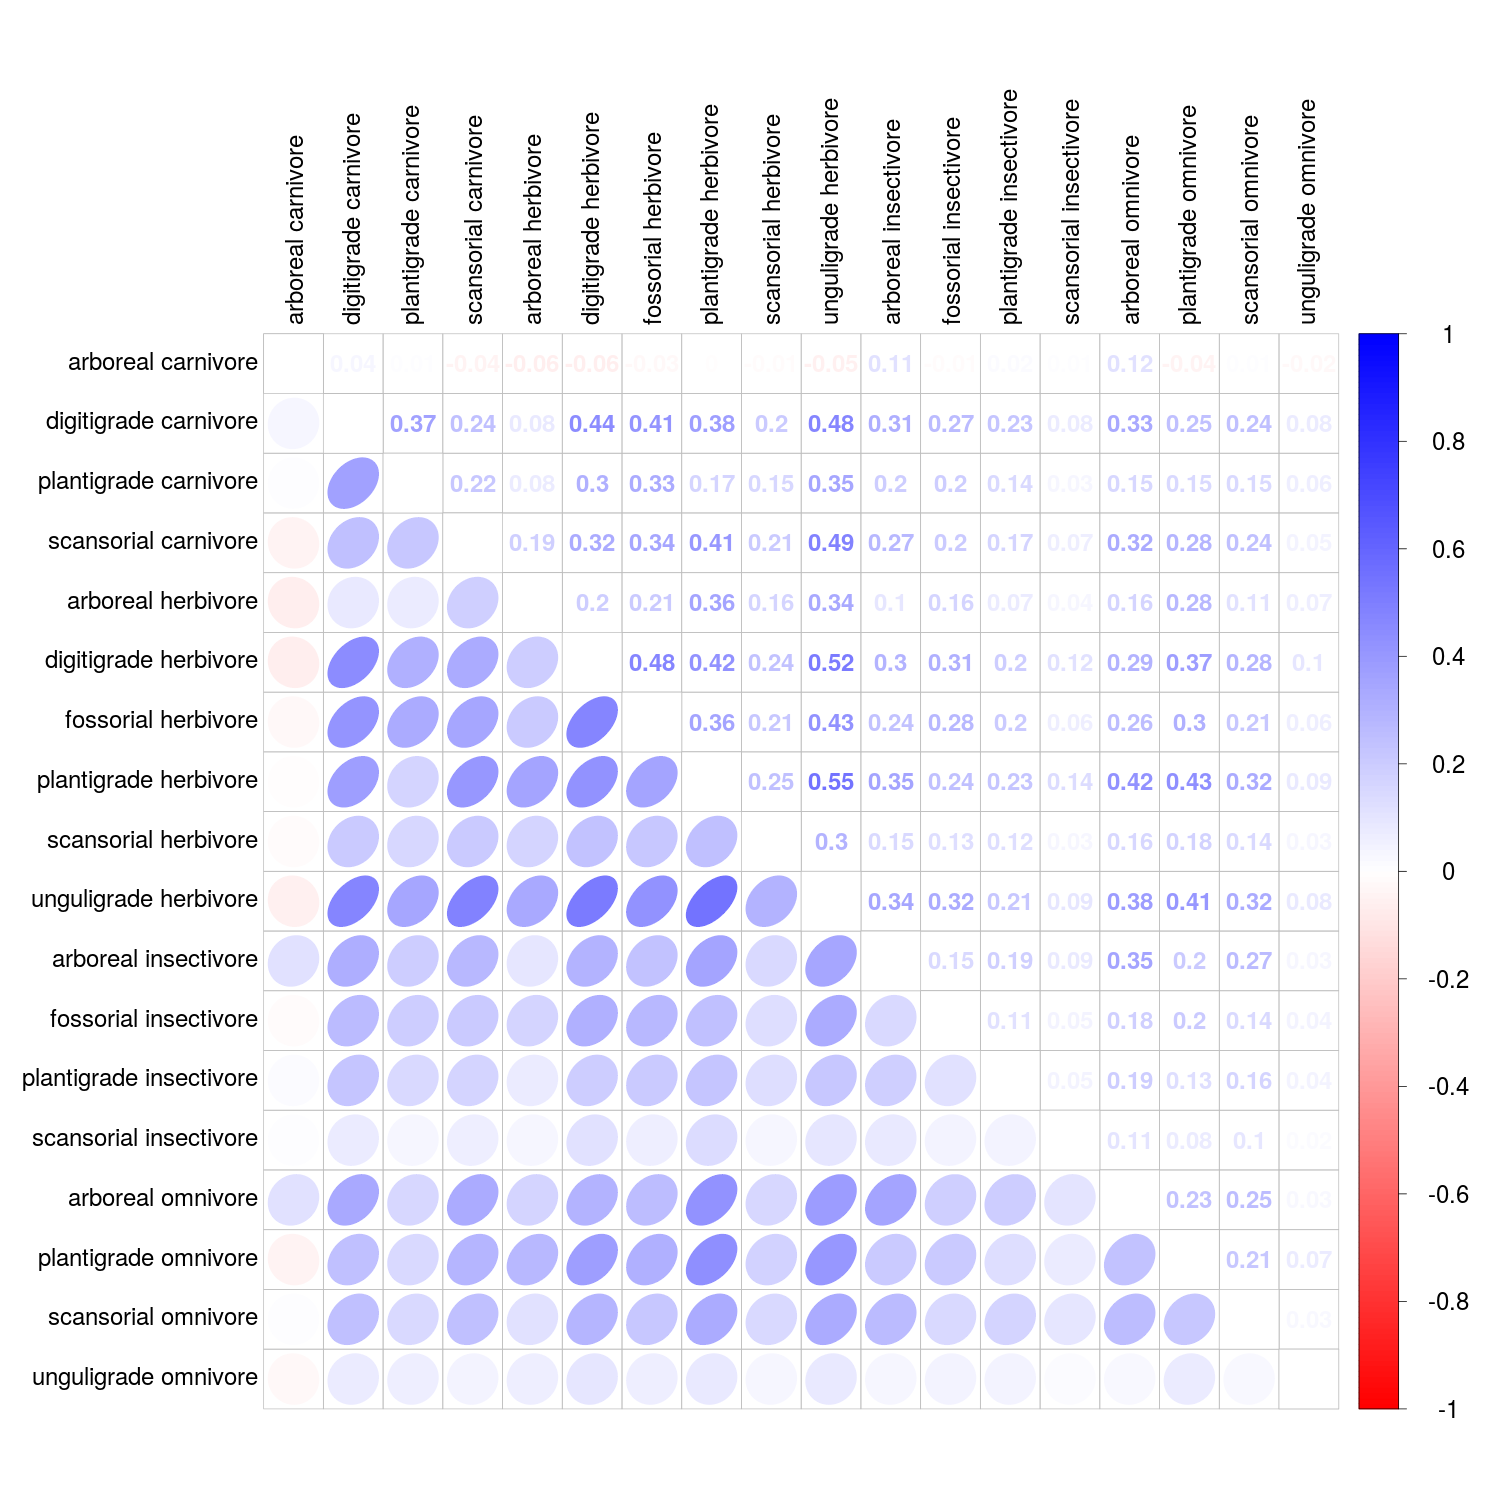
\includegraphics[width=\textwidth,height=\textheight,keepaspectratio=true]{chapter_coping/figure/origination_correlation}
  \caption[Estimated correlations in origination probability between ecotypes]{Posterior mean estimates of the correlations in origination probability between the mammal ecotypes. The lower triangle of the matrix is populated with ellipses corresponding to the level of correlation between the two ecotypes, while the upper triangle of the matrix corresponds to the mean estimated correlation between ecotypes. Darker values correspond to a greater magnitude of correlation with blue values corresponding to a positive correlation and red values a negative correlation.}
  \label{fig:origin_corr}
\end{figure}

\afterpage{\clearpage}
\begin{figure}[p]
  \centering
  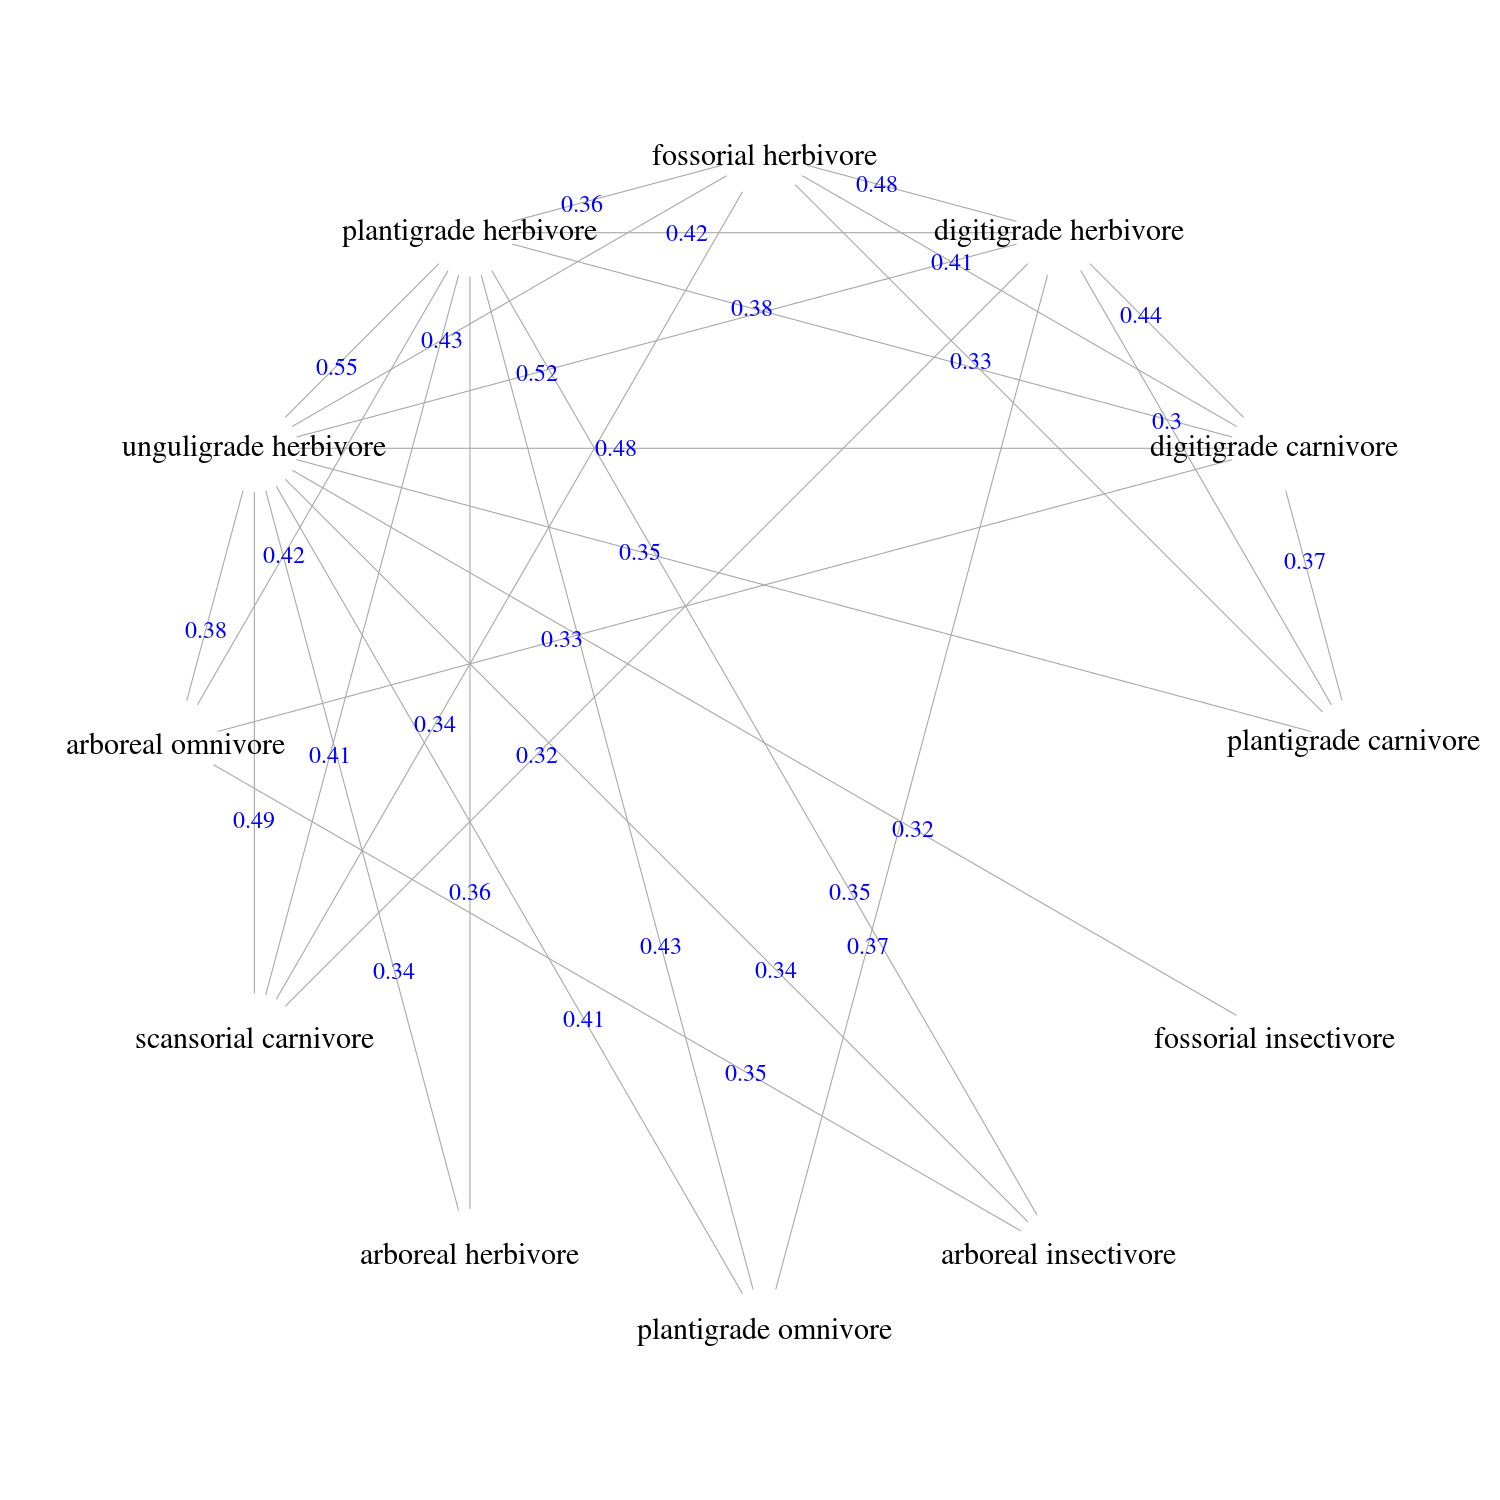
\includegraphics[width=\textwidth,height=\textheight,keepaspectratio=true]{chapter_coping/figure/origin_sig_corr}
  \caption[Ecotypes with strong correlations in origination probability]{Ecotypes that have a strong correlation in origination probability. These ecotypes have a greater than 95\% posterior probability of being positively correlated. The number plotted at the midpoint of each edge corresponds to the mean estimated correlation between those two ecotypes.}
  \label{fig:origin_corr_graph}
\end{figure}

\afterpage{\clearpage}
\begin{figure}[p]
  \centering
  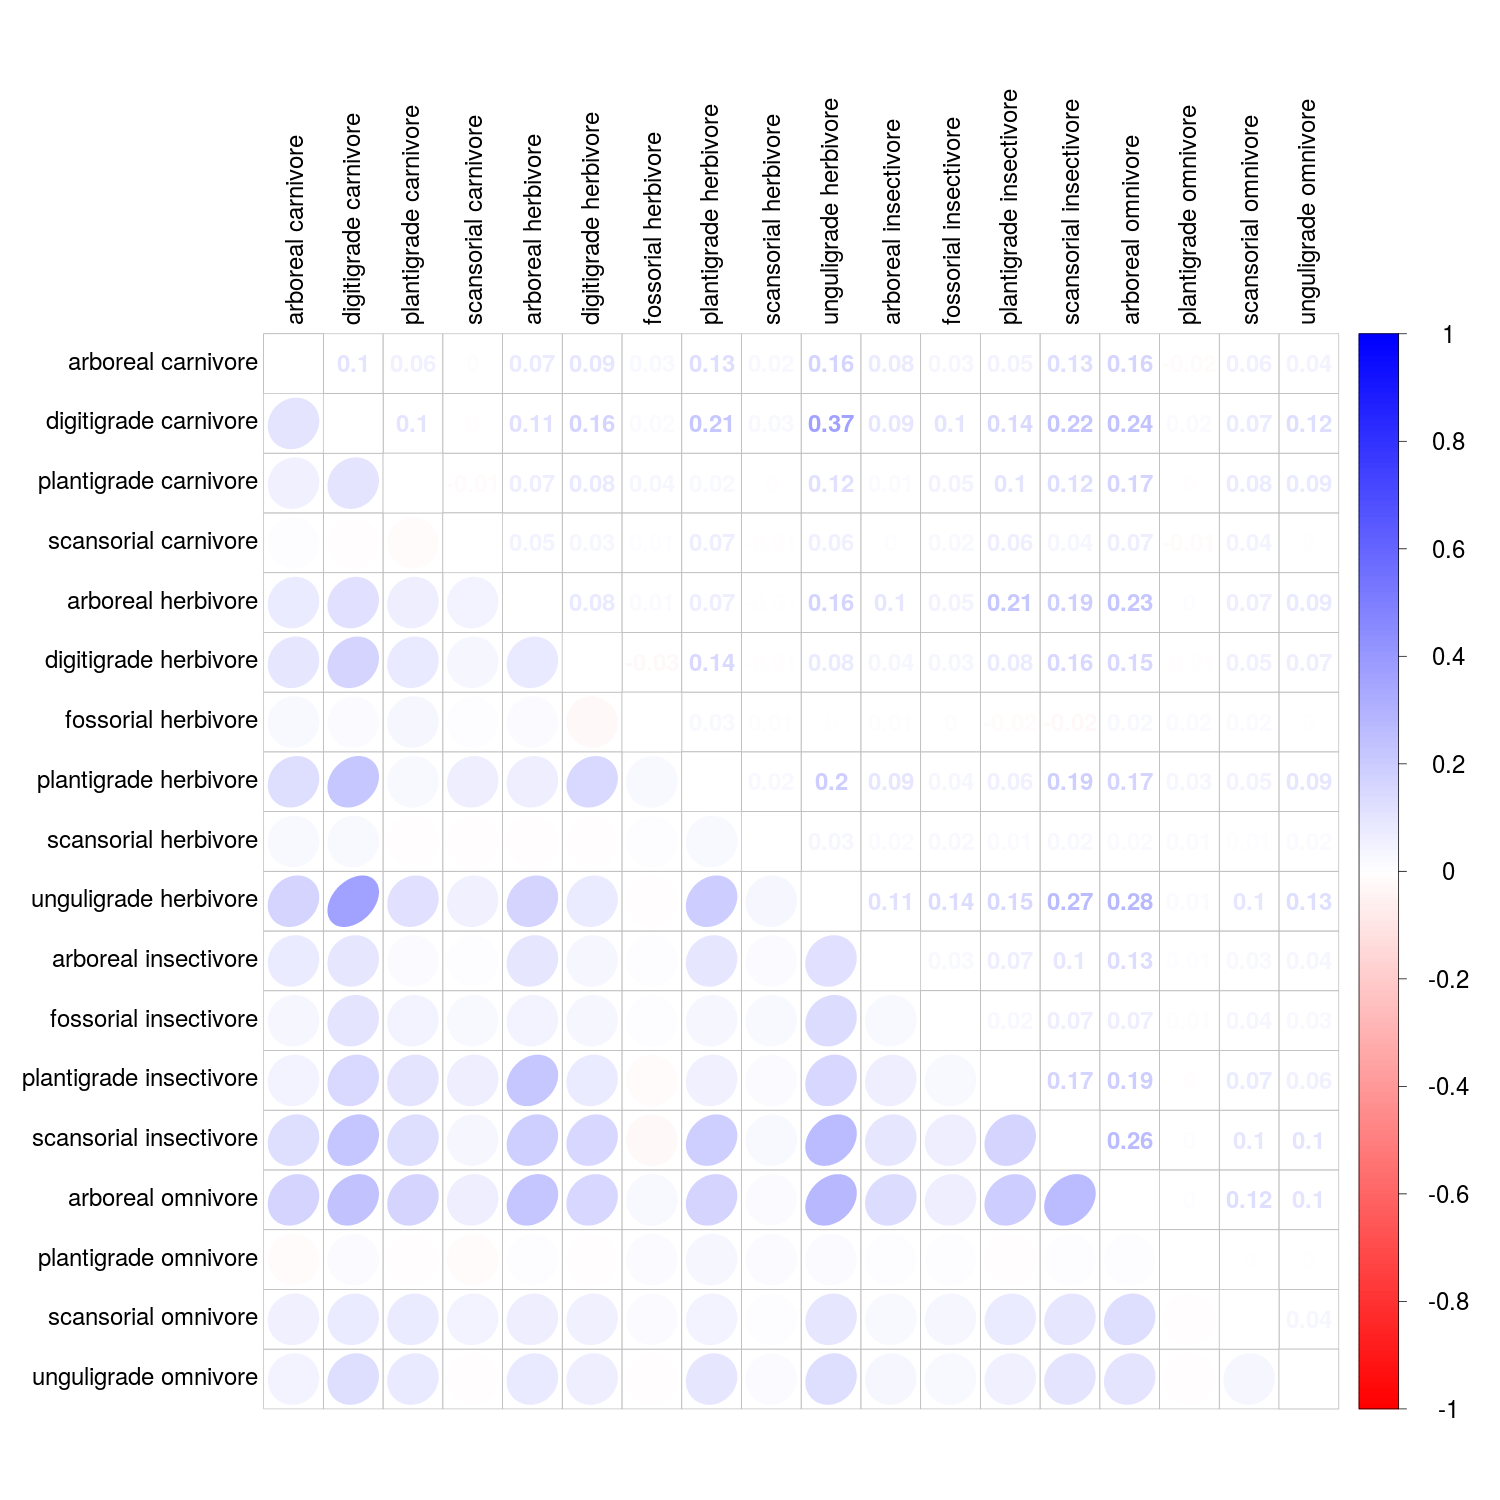
\includegraphics[width=\textwidth,height=\textheight,keepaspectratio=true]{chapter_coping/figure/survival_correlation}
  \caption[Estimated correlations in survival probability between ecotypes]{Posterior mean estimates of the correlations in survival probability between the mammal ecotypes. The lower triangle of the matrix is populated with ellipses corresponding to the level of correlation between the two ecotypes, while the upper triangle of the matrix corresponds to the mean estimated correlation between ecotypes. Darker values correspond to a greater magnitude of correlation with blue values corresponding to a positive correlation and red values a negative correlation.}
  \label{fig:survival_corr}
\end{figure}

\begin{figure}[ht]
  \centering
  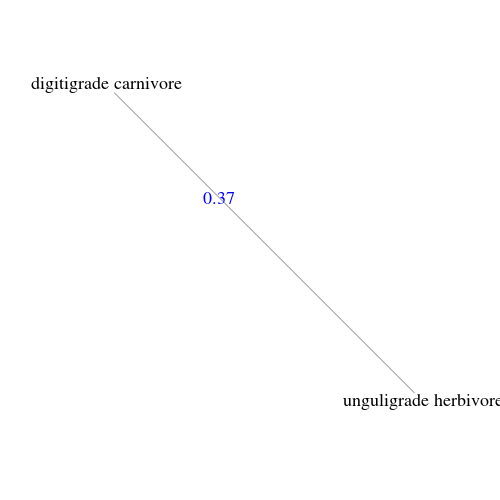
\includegraphics[width=\textwidth,height=0.4\textheight,keepaspectratio=true]{chapter_coping/figure/surv_sig_corr}
  \caption[Ecotypes with strong correlations in survival probability]{Ecotypes that have a strong correlation in survival probability. These ecotypes have a greater than 95\% posterior probability of being positively correlated. The number plotted at the midpoint of each edge corresponds to the mean estimated correlation between those two ecotypes.}
  \label{fig:surv_corr_graph}
\end{figure}



\subsection{Analysis of diversity}

All of the analyses of diversification and macroevolutionary rates has been done using only the birth-death model because of the model's better posterior predictive check performance (Fig. \ref{fig:ppc}).


The general pattern of the estimated North American total mammal diversity for the Cenozoic is ``stable'' in that diversity fluctuates around a constant mean standing diverisity, does not fluctuate wildly and rapidly over the Cenozoic, and demonstrates no sustained directional trends (Fig. \ref{fig:diversity_est}). In broad strokes, the first 15 or so million years of the Cenozoic are characterized by first an increase and then a decline in standing diversity at approximately 45-50 Mya (early-middle Eocene). Following this decline, standing diversity is broadly constant from 45 to 18 Mya (early Miocene). After this, there is a rapid spike in diversity followed by a slight decline in diversity up to the Recent. 

The pattern exhibited by the diversity history estimated in this study (Fig. \ref{fig:diversity_est}) has some major similarities with previous mammal diversity curves \citep{Alroy2009}: both diversity history estimates begin with an increase in diversity and most of the major increases in diversity are retained including the large diversity spike during the Miocene. Unlike subsampling based approaches to estimating diversity \citep{Alroy2010c}, I'm able to interpolate over unsampled/poorly sampled time periods because of how the hierarchical model can share information across the different units \cite{Gelman2013d}; for cases like unsampled temporal bins, this may lead to estimates with high uncertainty, but that is preferable to no estimate at all. Finally, the Bayesian framework here gives a distribution of possible estimates of diversity allowing for direct inspection of the uncertainty of our inferences, something that is preferable to both traditional and resampling based confidence interval estimates \citep{Gelman2013d}. Note that my time series of estimated diversity begins at a slightly different point than that used by Alroy \citep{Alroy2009} and that the time intervals used by Alroy \citep{Alroy2009} are slightly shorter than those used here, so this may cause some of the minor differences between the curves. Also, please note that the diversity values are plotted at the ``ceiling'' of each temporal interval and not at the midpoint (Fig. \ref{fig:diversity_est}).

When viewed through the lens of diversification rate, some of the structure behind the estimated diversity history begins to take shape (Fig. \ref{fig:diversity_rate}). For most of the Cenozoic, the diversification rate hovers around zero, punctuated by both positive and negative spikes. The largest spike in diversification rate is at 16 Mya, which is early Oligocene (Fig. \ref{fig:diversity_rate}). Other notable increases in diversification rate occur at 56, 46, 22, 18, and 6 Mya (Table \ref{tab:div_peak}), though the last of these may be due to edge effects surrounding the partial-identifiability of \(p_{t = T}\). Notable decreases in diversification rate occur at 54, 50, 48, 44, 40, 34, 30, 24, 20, 16, 12, and 8 Mya (Table \ref{tab:div_peak}), meaning that diversification rate has more major decreases than increases. While diversification rates significantly lower than average are more common than diversification rates greater than average, when positive diversification rates have a greater magnitude than most periods of low or negative diversification (Fig. \ref{fig:diversity_rate}). Given that diversification rate more closely resembles origination rate than extinction rate (Fig. \ref{fig:diversity_rate}, \ref{fig:origin_rate}, \ref{fig:extinct_rate}), these decreases in diversification rate may be indicative of ``depletions'' (failure to replace extinct taxa) rather than pulses of extinction. 

The estimates from this study of per capita origination and extinction rates for the entire species pool (Fig. \ref{fig:origin_rate}, \ref{fig:extinct_rate}) are very different from the origination and extinction rates estimated by Alroy \citep{Alroy2009}. The two most striking differences are the very different estimates of extinction rate between the two studies and the very different scales of the origination rate estimates. This may be due to the fundamentally different way these rates are calculated, and how the diversification process was modeled. The per capita rates estimated in this study follow straight from the definition of a per capita rate (e.g. number of originations between time \(t\) and \(t + 1\) divided by the diversity at time \(t\)) while the rates calculated by Alroy \citep{Alroy2009} are based on log ratios of standing diversity.

The comparison between per capita origination and extinction rate estimates reveals how diversification rate is formed (Fig. \ref{fig:origin_rate}, \ref{fig:extinct_rate}). As expected given previous inspection of the ecotype specific estimates of origination and survival probabilities from the birth-death model, diversification rate seems most driven by changes in origination rate as opposed to extinction rate. Extinction rate, on the other hand, demonstrates an almost saw-toothed pattern around a constant mean (Fig. \ref{fig:extinct_rate}). These results are broadly consistent with those from previous analyses of North American mammals diversity and diversification \citep{Alroy1996a,Alroy2000g,Alroy2009}.

\afterpage{\clearpage}
\begin{figure}[p]
  \begin{subfigure}[b]{0.45\textwidth}
    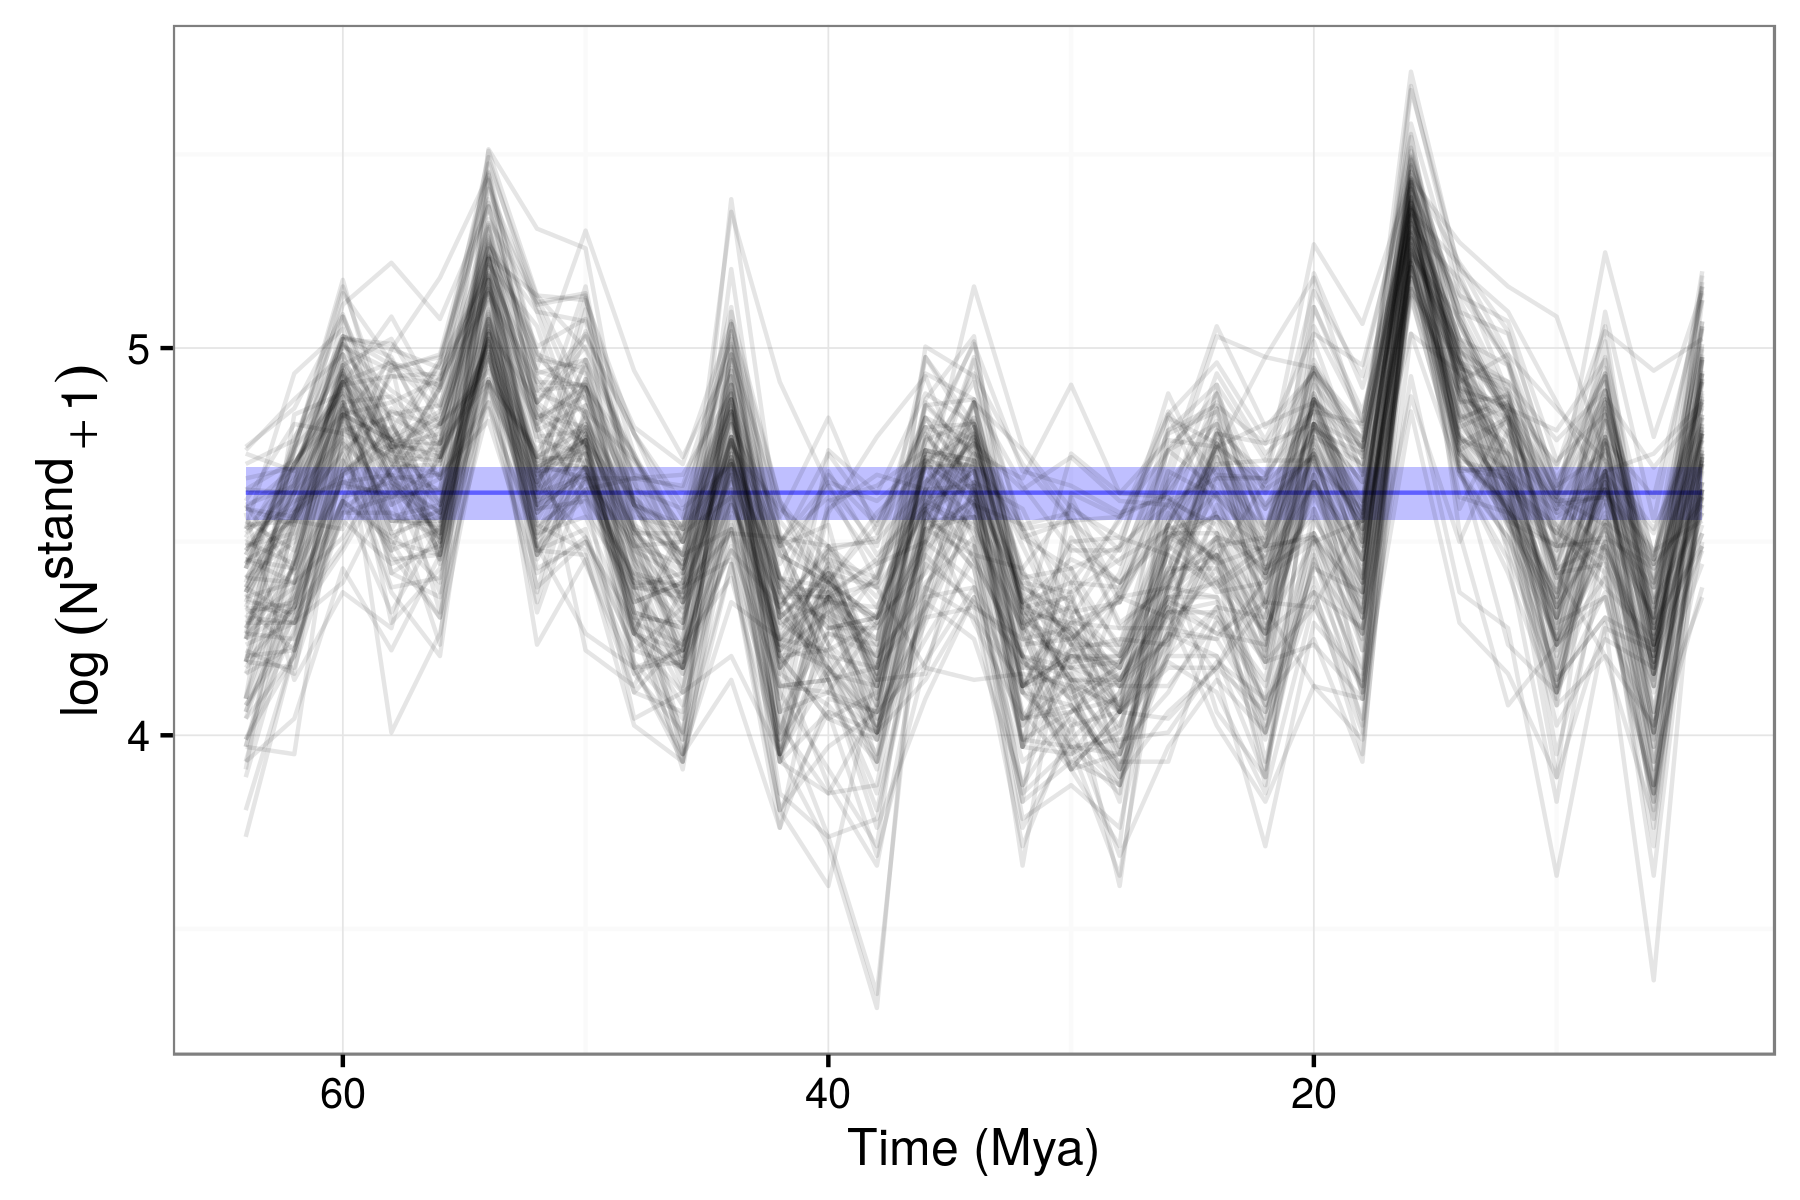
\includegraphics[width=\textwidth,height=0.4\textheight,keepaspectratio=true]{chapter_coping/figure/log_diversity}
    \caption{Log diversity}
    \label{fig:diversity_est}
  \end{subfigure}
  \begin{subfigure}[b]{0.45\textwidth}
    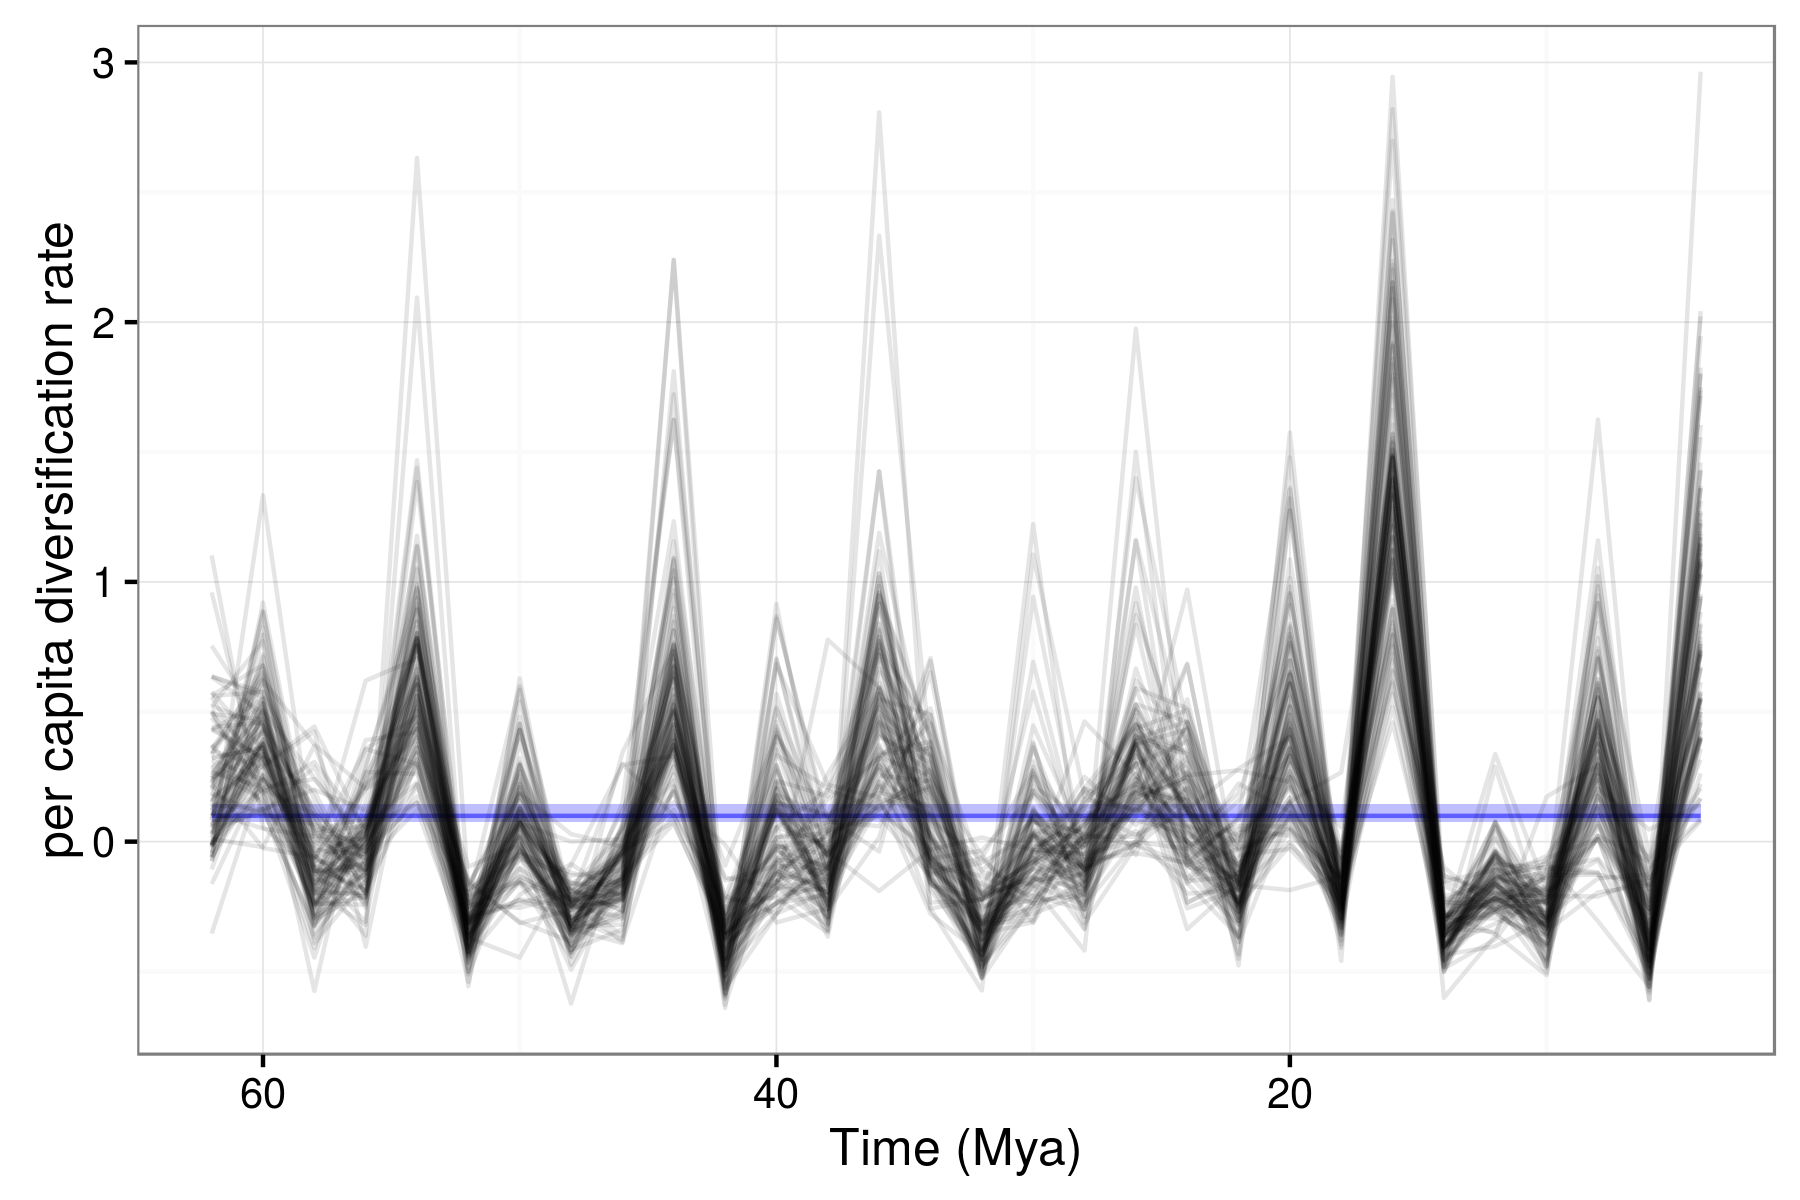
\includegraphics[width=\textwidth,height=0.4\textheight,keepaspectratio=true]{chapter_coping/figure/div_rate}
    \caption{Diversification rate}
    \label{fig:diversity_rate}
  \end{subfigure}

  \begin{subfigure}[b]{0.45\textwidth}
    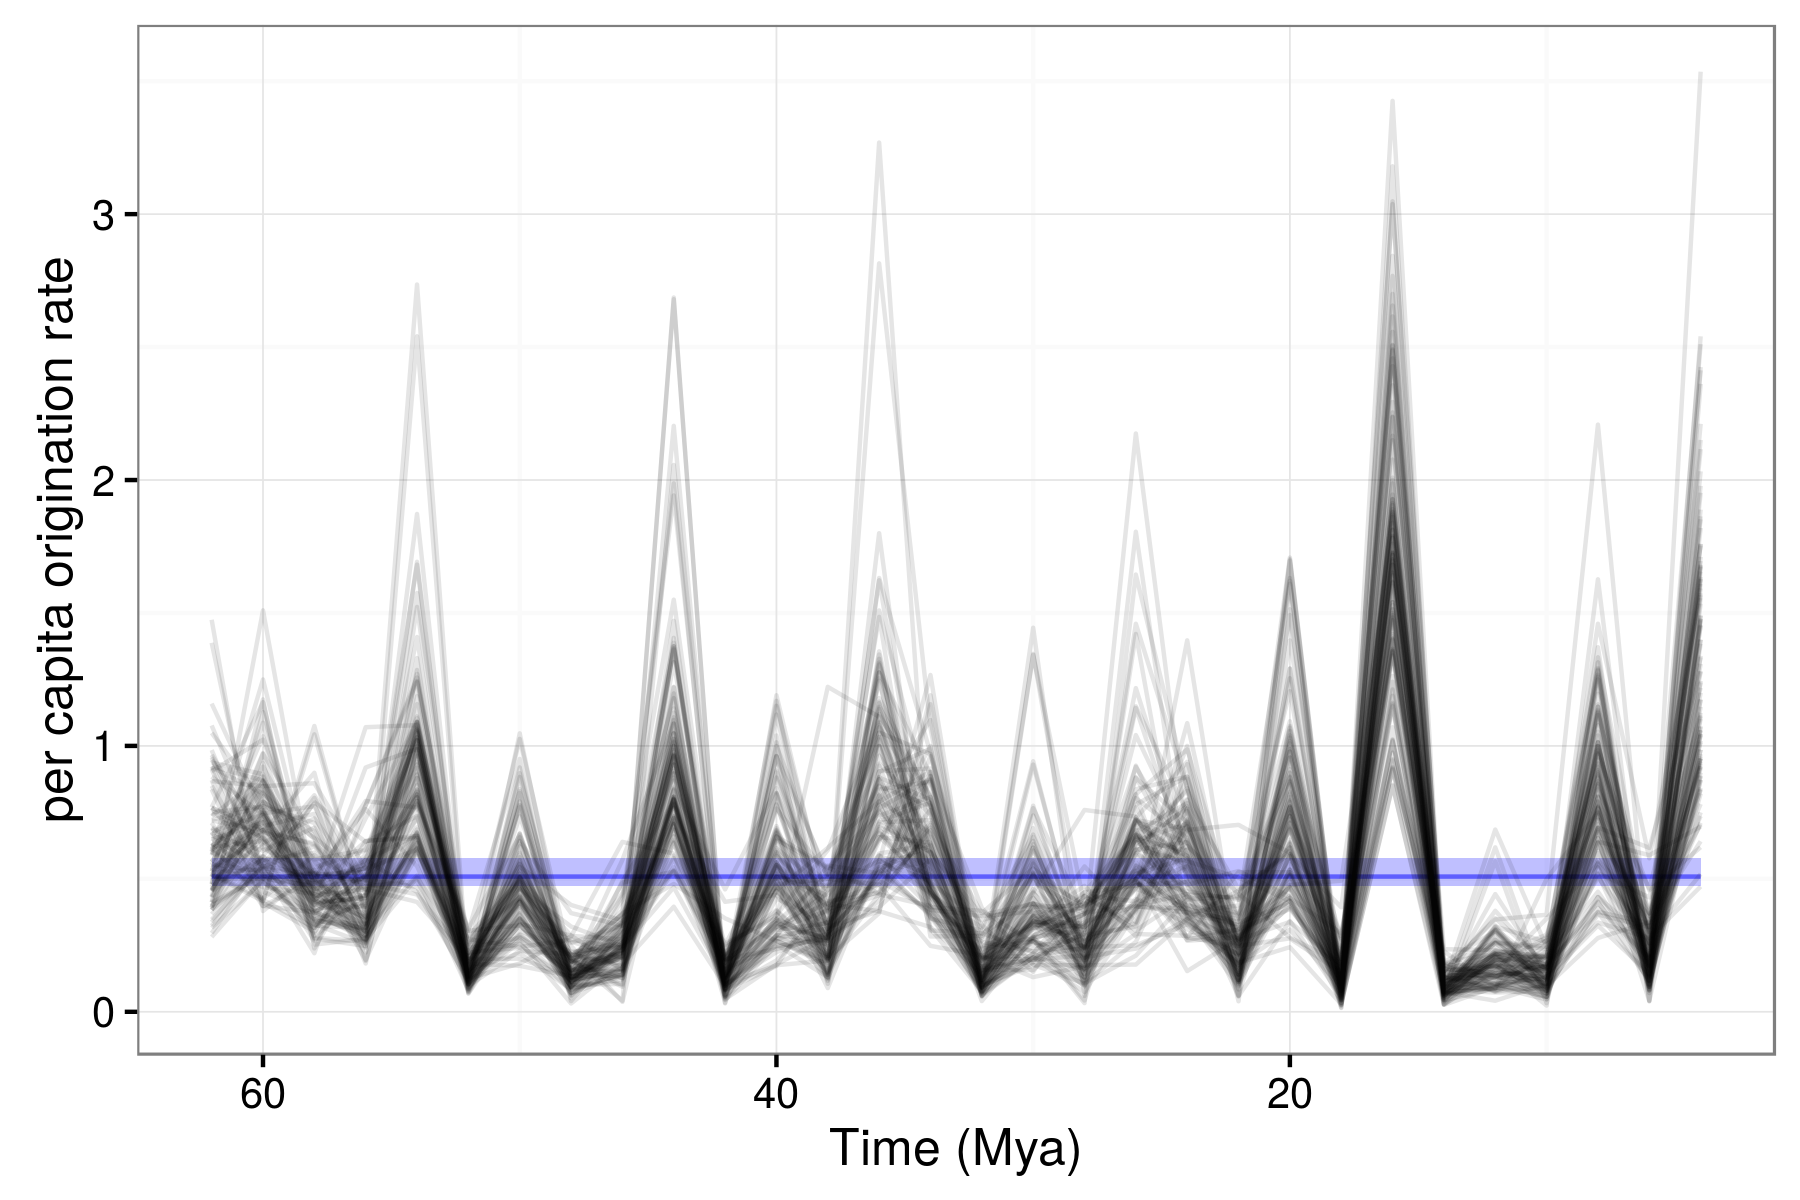
\includegraphics[width=\textwidth,height=0.4\textheight,keepaspectratio=true]{chapter_coping/figure/orig_rate}
    \caption{Origination rate}
    \label{fig:origin_rate}
  \end{subfigure}
  \begin{subfigure}[b]{0.45\textwidth}
    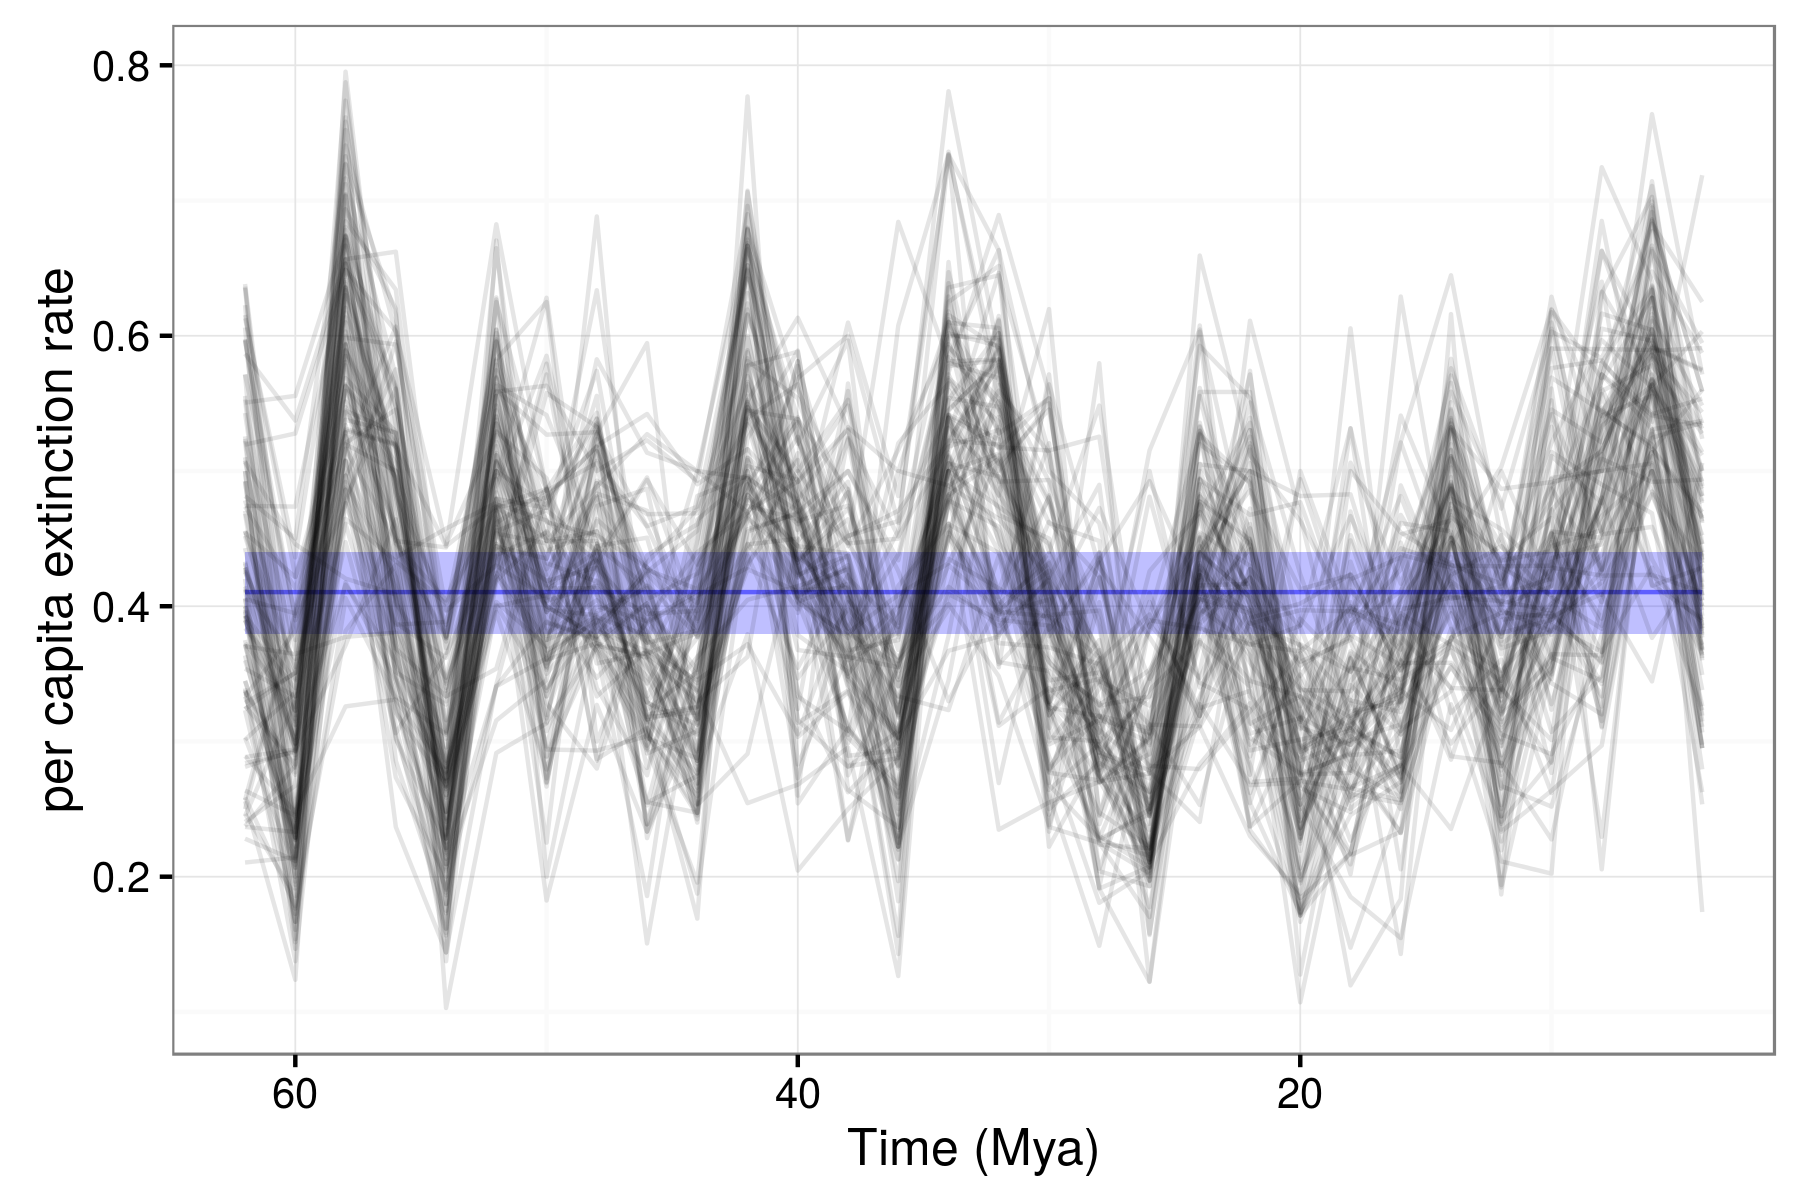
\includegraphics[width=\textwidth,height=0.4\textheight,keepaspectratio=true]{chapter_coping/figure/death_rate}
    \caption{Extinction rate}
    \label{fig:extinct_rate}
  \end{subfigure}
  \caption[Estimated mammal log-diversity and macroevolutionary rates for the Cenozoic]{Posterior estimates of the time series of Cenozoic North American mammal diversity and it's characteristic macroevolutionary rates; all estimates are from the birth-death model and 100 posterior draws are plotted to indicate the uncertainty in these estimates. The blue horizontal strip corresponds to the 80\% credible interval of estimated mean standing diversity, diversification rate, origination rate, and extinction rate respectively; the median estimate is also indicated. What is also plotted is the  The dramatic differences between diversity estimates at the first and second time points and the penultimate and last time points in this series are caused by well known edge effects in discrete-time birth-death models caused by \(p_{\_, t = 1}\) and \(p_{\_, t = T}\) being partially unidentifiable \citep{Royle2008}; the hierarchical modeling strategy used here helps mitigate these effects but they are still present \citep{Gelman2013d,Royle2008}. Diversification rate is in units of species gained per species present per time unit (2 My), origination rate is in units of species originating per species present per time unit, and extinction rate is in units of species becoming extinct per species present per time unit.}
  \label{fig:macro_values}
\end{figure}

\begin{table}[ht]
  \centering
  \caption[Posterior probability estimates of a peak in diversity, diversification]{Posterior probabilities of diversity \(N^{stand}_{t}\) or diversification rate \(D^{rate}_{t}\) being greater than average standing diversity \(\overline{N^{stand}}\) or average diversification rate \(\overline{D^{rate}}\) for the whole Cenozoic. The ``Time'' column corresponds to the top of each of the temporal bins. Diversification rate can not be estimated for the last time point because it is unknown how many more species originated or went extinct following this temporal bin. The estimates are from the birth-death model.}
  \label{tab:div_peak}
  \begin{tabular}{ r r r }
    \hline
    Time (Mya) & \(P(N^{stand}_{t} > \overline{N^{stand}})\) & \(P(D^{rate}_{t} > \overline{D^{rate}})\) \\ 
    \hline
    64.00 & 0.07 & 0.63 \\ 
    62.00 & 0.28 & 0.94 \\ 
    60.00 & 0.86 & 0.13 \\ 
    58.00 & 0.68 & 0.18 \\ 
    56.00 & 0.62 & 0.99 \\ 
    54.00 & 1.00 & 0.00 \\ 
    52.00 & 0.68 & 0.41 \\ 
    50.00 & 0.80 & 0.00 \\ 
    48.00 & 0.12 & 0.04 \\ 
    46.00 & 0.01 & 0.98 \\ 
    44.00 & 0.64 & 0.00 \\ 
    42.00 & 0.02 & 0.47 \\ 
    40.00 & 0.03 & 0.08 \\ 
    38.00 & 0.00 & 0.89 \\ 
    36.00 & 0.40 & 0.46 \\ 
    34.00 & 0.52 & 0.00 \\ 
    32.00 & 0.02 & 0.27 \\ 
    30.00 & 0.06 & 0.09 \\ 
    28.00 & 0.02 & 0.88 \\ 
    26.00 & 0.22 & 0.39 \\ 
    24.00 & 0.38 & 0.03 \\ 
    22.00 & 0.09 & 0.96 \\ 
    20.00 & 0.81 & 0.00 \\ 
    18.00 & 0.29 & 1.00 \\ 
    16.00 & 1.00 & 0.00 \\ 
    14.00 & 0.95 & 0.02 \\ 
    12.00 & 0.80 & 0.01 \\ 
    10.00 & 0.13 & 0.83 \\ 
    8.00 & 0.67 & 0.00 \\ 
    6.00 & 0.02 & 1.00 \\ 
    4.00 & 0.91 &  \\ 
    \hline
  \end{tabular}
\end{table}



\afterpage{\clearpage}
\begin{figure}[p]
  \centering
  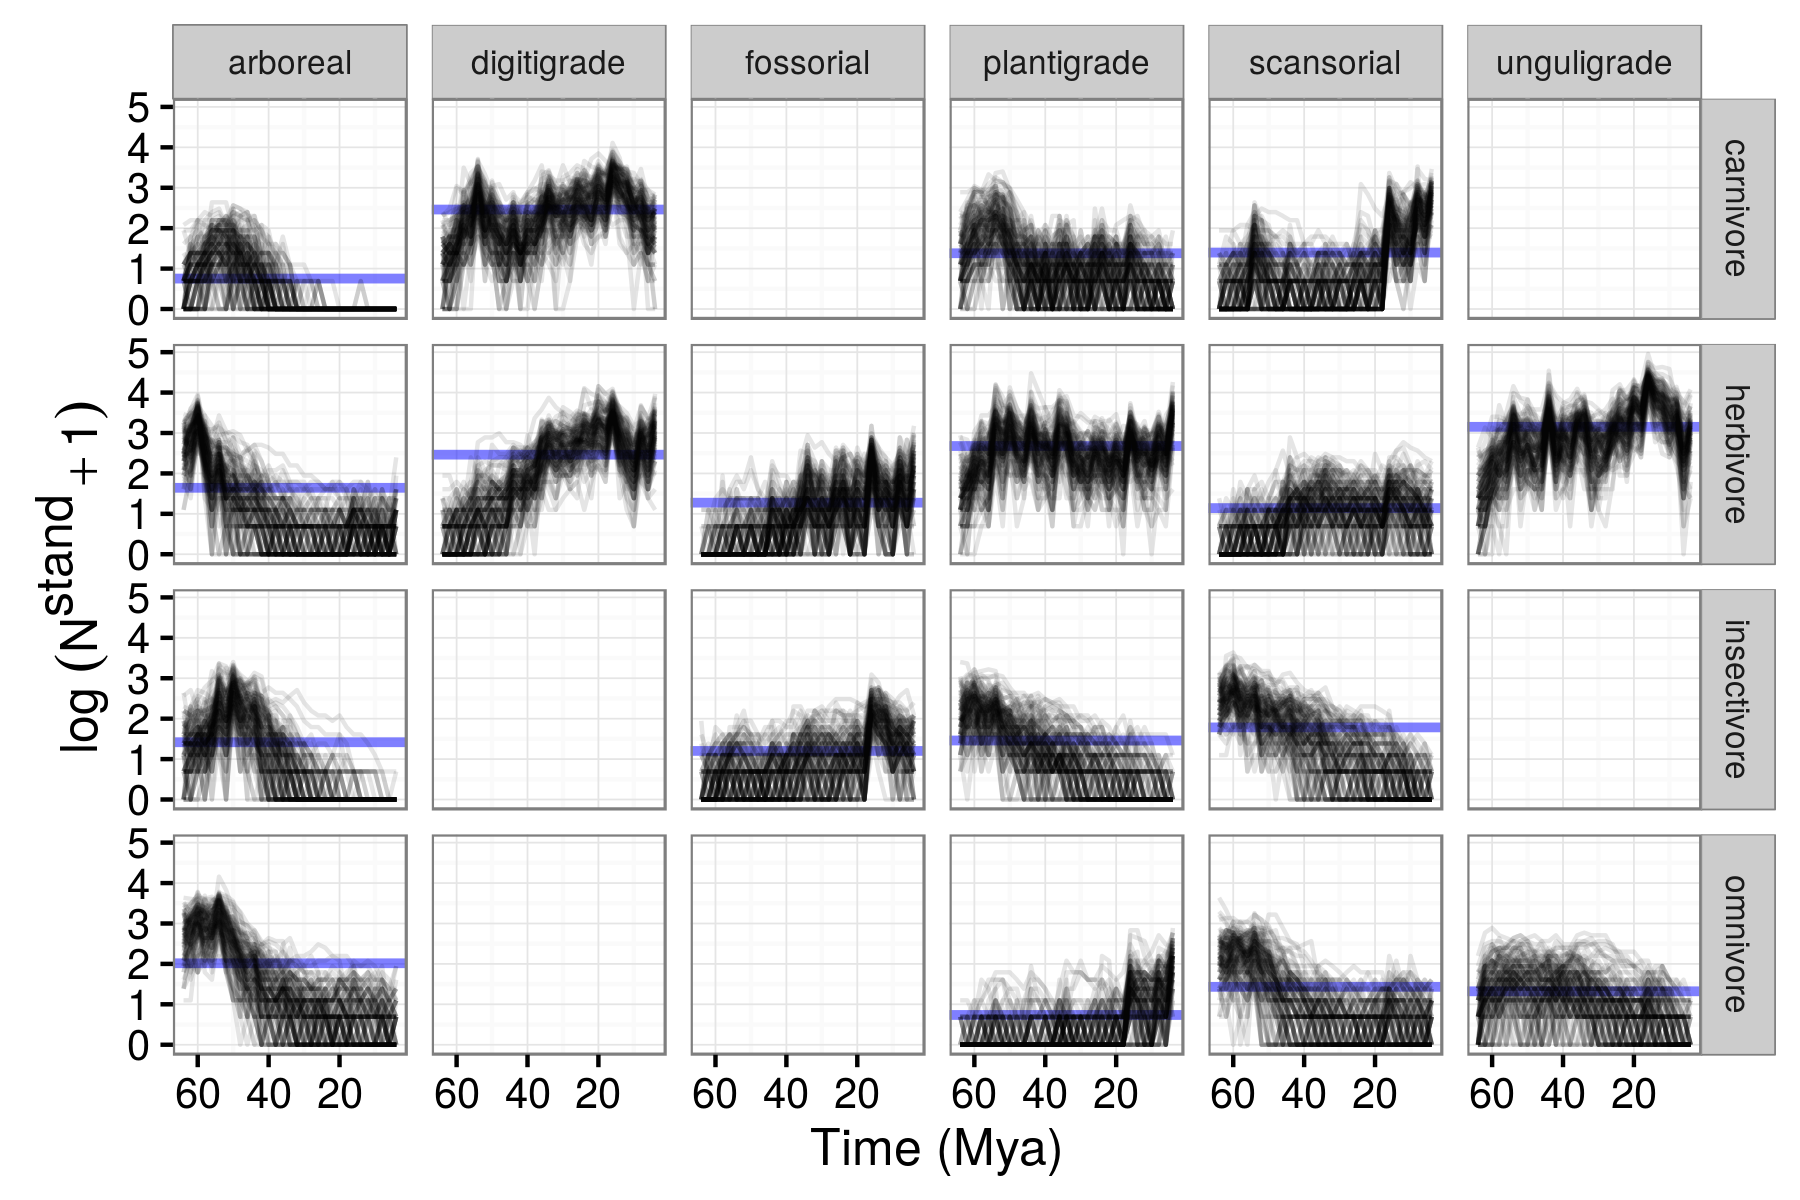
\includegraphics[width=\textwidth,height=\textheight,keepaspectratio=true]{chapter_coping/figure/ecotype_diversity}
  \caption[Estimated mammal ecotype log-diversity for the Cenozoic]{Posterior of standing log-diversity of North American mammals by ecotype for the Cenozoic as estimated from the birth-death model; 100 posterior draws are plotted to indicate the uncertainty in these estimates and what is technically plotted is log of diversity plus 1.}
  \label{fig:ecotype_diversity}
\end{figure}

Diversity partitioned by ecotype reveals a lot of the complexity behind the pattern of mammal diversity for the Cenozoic (Fig. \ref{fig:ecotype_diversity}). 

Arboreal ecotypes obtain peak diversity early in the Cenozoic and then decline for the rest of the time series, becoming increasingly rare or absent as time approaches the Recent (Fig. \ref{fig:ecotype_diversity}). Arboreal herbivores and omnivores obtain peak diversity at the beginning of the Cenozoic then go into decline while remaining a small part of the species pool, while arboreal carnivores and insectivores obtain peak diversity 52-50 Mya and then quickly decline and become extremely rare or entirely absent from the species pool. This is consistent with increasing extinction risk in the Neogene compared to the Paleogene as proposed by Smits \citep{Smits2015b}.

The diversity of digitigrade and unguligrade herbivores increases over the Cenozoic (Fig. \ref{fig:ecotype_diversity}). In contrast, plantigrade herbivore diversity does not have a single, broad-strokes pattern; instead, diversity increases, decreases, and may have then increased till the Recent. In contrast, fossorial and scansorial herbivores demonstrate a much flatter history of diversity, with a slight increase in diversity that over time is more pronounced among fossorial taxa than scansorial taxa. The expansion of digitigrade and unguligrade herbivores over the Cenozoic is consistent with the gradual expansion of grasslands which these ecotypes are better adapted to than closed environments \citep{Blois2009,Stromberg2005}.

Digitigrade carnivores have a multi-modal diversity history, with peaks at 54-52 and 12-10 Mya (Fig.\ref{fig:ecotype_diversity}). Between these two peaks digitigrade carnivore diversity dips below average diversity following the first peak and then grows slowly until the second peak. Plantigrade carnivores obtain peak diversity in the early Cenozoic and then maintain a relatively stable diversity until another peak at the end of the Cenozoic. The generally flat diversity history of digitigrade carnivores lacks any sustained temporal trends and seems to reflect previous findings of limited diversity in spite of constant turnover and morphological evolution \citep{Valkenburgh1999,Silvestro2015b,Slater2015c}

There are some broad similarities in diversity histories of insectivorous and omnivorous taxa. The diversity histories of arboreal, plantigrade, and scansorial insectivorous taxa all demonstrate a decreasing pattern with time, while fossorial insectivores have a flat diversity history with a peak approximately 10 Mya (Fig. \ref{fig:ecotype_diversity}). Arboreal and scansorial omnivores decrease in diversity from their initial peaks early in the Cenozoic, and plantigrade omnivores have a generally flat diversity history with a sudden peak in diversity late in the Cenozoic (Fig. \ref{fig:ecotype_diversity}). Unguligrade omnivores also demonstrate a possible decrease in diversity over the Cenozoic, but not as clearly as arboreal and scansorial omnivores.


The waxing and waning of the mammal ecotypes is obvious when comparing changes to estimated relative log-mean of diversity (Fig. \ref{fig:ecotype_relative}). While ecotype diveristy does appear to change gradually, there are definite changes to the relative contributions of the ecotypes to the regional species pool. All arboreal ecotypes clearly decrease in relative diversity over the Cenozoic. In contrast the the digitigrade herbivore, fossorial herbivore, scansorial herbivore, and unguligrade herbivore ecotypes which increase in relative diversity over the Cenozoic. The digitigrade carnivore ecotype increases in relative diveristy until approximately the start of the Neogene, after which it maintains a generally constant relative diveristy; this is consistent with previous observations of constant or density-dependent diversity of the canid guild for the Neogene \citep{Valkenburgh1999,Silvestro2015b,Slater2015c}, a guild that overlaps with the digitigrade carnivore ecotype. Plantigrade herbivores remain a constant relative contribution to ecotypic diveristy. These results support the hypothesis of a gradual transition from the early Paleogene with a region with more avaliable habitat for aboreal taxa and less avaliable habitat for many digitigrade and unguligrade taxa, to an environment where arboreal taxa are absent from the species pool and digitigrade and unguligrade taxa are much more dominant (Fig. \ref{fig:ecotype_relative}). It is the relative contributions of digitgrade carnivores, digitigrade herbivores, and unguligrade herbivores which really shape the regional species pool of the Neogene. 


\afterpage{\clearpage}
\begin{figure}[p]
  \centering
  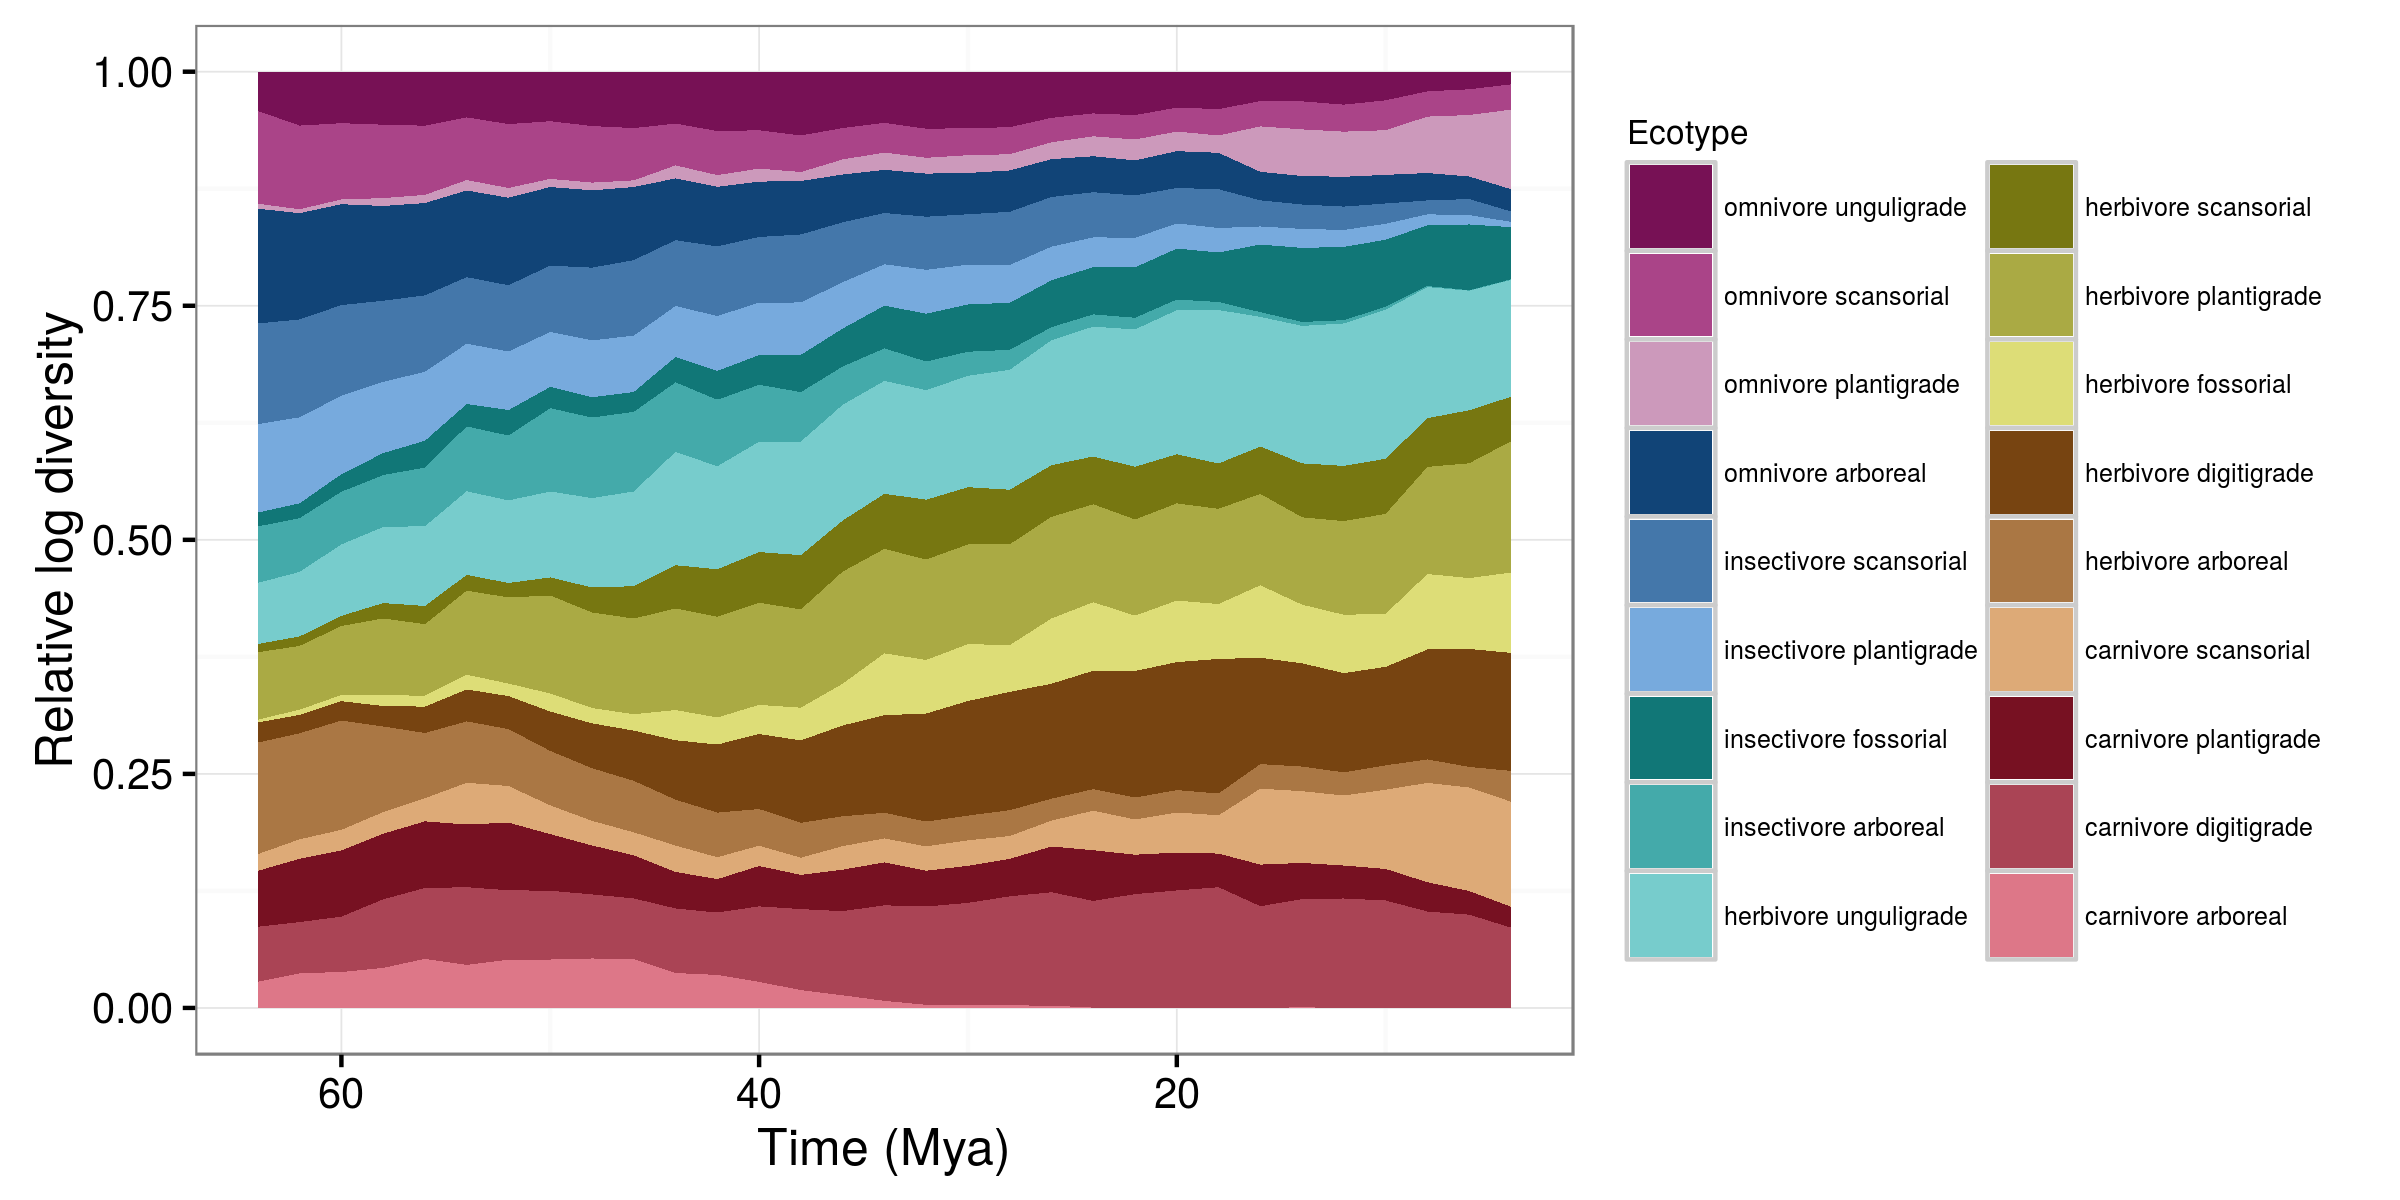
\includegraphics[width=\textwidth,height=\textheight,keepaspectratio=true]{chapter_coping/figure/relative_diversity}
  \caption[Relative mammal ecotype log-diversity for the Cenozoic]{Mean posterior estimate of relative log standing diveristy of 18 North American mammal ecotypes for the Cenozoic. These estimates are calculated from 100 posterior estimates of the true occurrence matrix \(z\) as estimated from the birth-death model.}
  \label{fig:ecotype_relative}
\end{figure}


Many of the estimated ecotype-specific diversity histories share a similar increase in diversity in the late Cenozoic, 16-14 Mya (Fig. \ref{fig:ecotype_diversity}). These increases are either sustained or temporary and are seen in digitigrade carnivores, plantigrade carnivores, scansorial carnivores, unguligrade herbivores, fossorial insectivores, and plantigrade omnivores.

When ecotype diversity is decomposed into per capita origination (Fig. \ref{fig:ecotype_birth}) and per capita extinction rates (Fig. \ref{fig:ecotype_death}) the way in which their diversity developed can be explained. For ecotype-specific origination and extinction rates, the number of origination or extinction events for each ecotype was calculated and that number was divided by the total standing diversity of all mammals at the time. 

As should be expected from the comparisons between estimates of origination and survival probability, origination rates have a much greater range of values with a few very large spikes that line up with the spikes in over all diversification rate (Fig. \ref{fig:diversity_rate}). Importantly, the source of the massive increase in diversification rate at 16 Mya can be attributed almost solely to the origination of unguligrade herbivores (Fig. \ref{fig:ecotype_birth}). Additionally, by decomposing origination rate by ecotype, it is possible to identify a few possible cross-ecotype increases in origination rate. For example, digitigrade carnivores, digitigrade herbivores, and plantigrade herbivores share a lot of increases in origination rate with unguligrade herbivores; these are all ecotypes that demonstrate an obvious increase in diversity during the Paleogene and then maintain relatively high diversity through out the Neogene (Fig. \ref{fig:ecotype_diversity}).

In contrast to ecotype-specific per capita origination rates which demonstrate distinct peaks, the estimates of ecotype-specific per capita rates are more of a smear (Fig. \ref{fig:ecotype_death}). There are few increases in extinction rate that are shared across ecotypes. The per captia extinction rates of digitigrade, plantigrade, and unguligrade herbivores are lower in Paleogene than the Neogene. This result is interpreted to mean that as the diversity of these three ecotypes was increasing, the number of extinction events was also increasing. Also, the per capita extinction rate of arboreal taxa is higher in the Paleogene than the Neogene. While this result may seem odd considering the observed diversity pattern for these ecotypes (Fig. \ref{fig:ecotype_diversity}), I argue that this result is actually extremely intuitive: if there are no species of that ecotype originating or present, than there can be extinctions. This result highlights the distinction between extinction risk and extinction rate; an ecotype can have a high extinction risk, but if that ecotype is not present in the species pool in the first place than it has no associated extinction rate. 

\begin{figure}[ht]
  \centering
  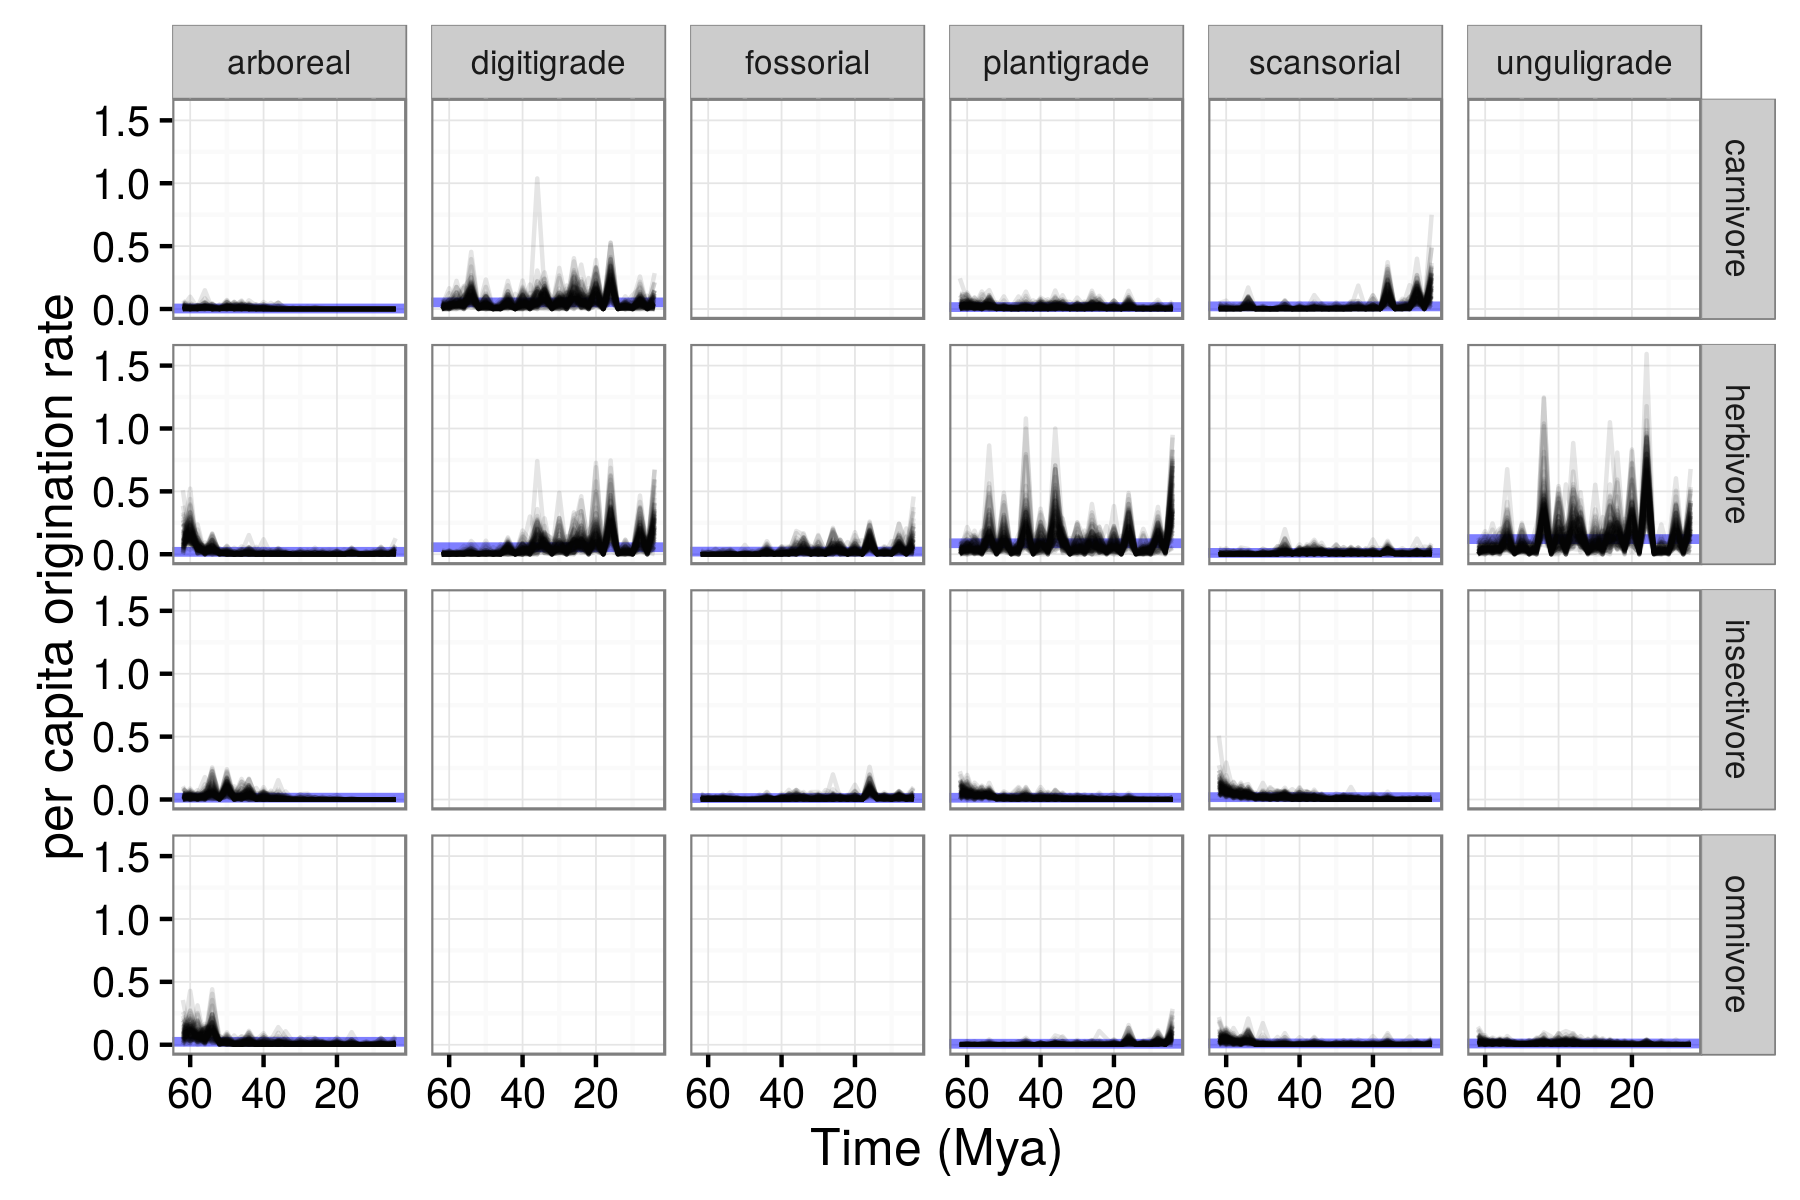
\includegraphics[width=\textwidth,height=0.4\textheight,keepaspectratio=true]{chapter_coping/figure/birth_eco}
  \caption[Estimated per capita origination rates by mammal ecotype]{Posterior estimates of the per capita origination rates for each ecotype, plotted at the bin they originate from. These rates are calculated as the number of origination events for that ecotype from one time point to the next, divided by the standing diversity of all mammals at the initial time point. 100 posterior draws are plotted to indicate the uncertainty in these estimates.}
  \label{fig:ecotype_birth}
\end{figure}

\begin{figure}[ht]
  \centering
  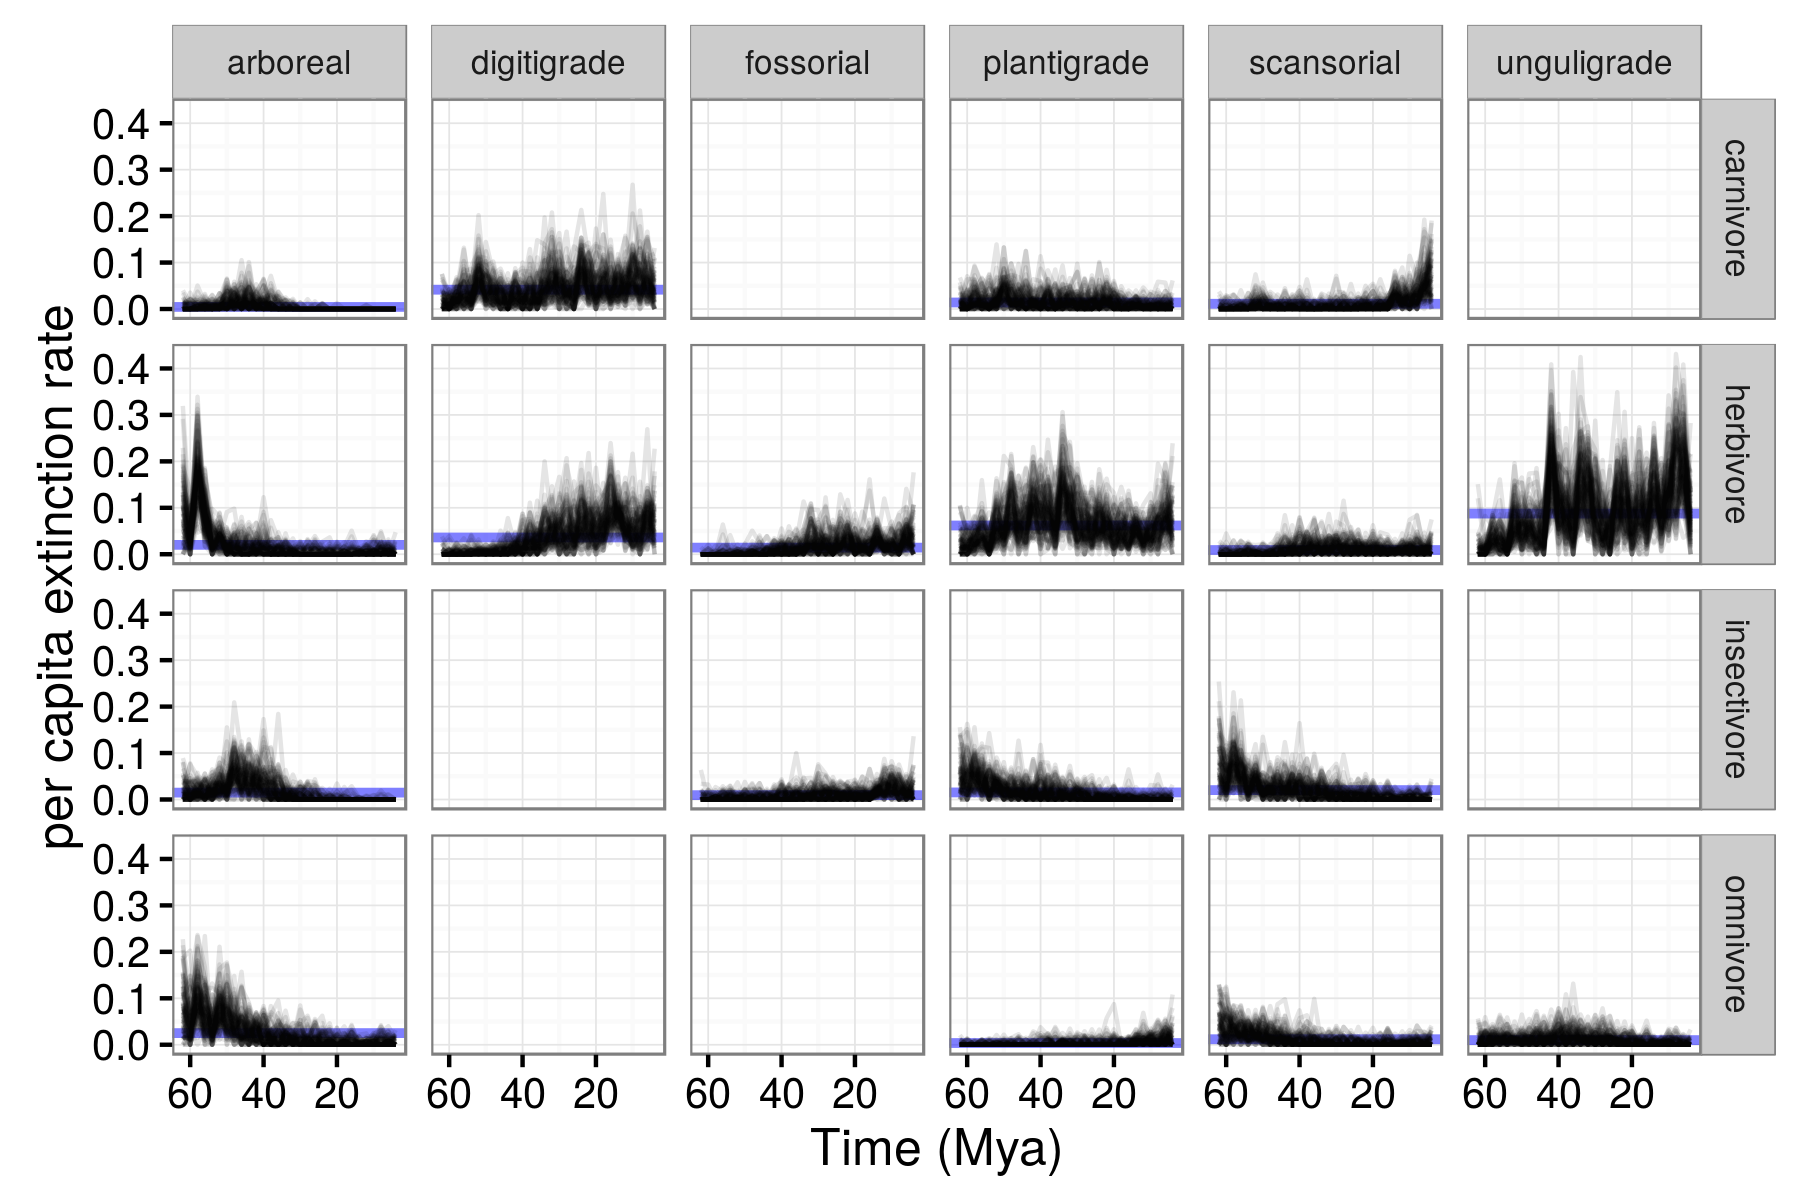
\includegraphics[width=\textwidth,height=0.4\textheight,keepaspectratio=true]{chapter_coping/figure/death_eco}
  \caption[Estimated per capita extinction rates by mammal ecotype]{Posterior estimates of the per capita extinction rates for each ecotype, plotted at the bin they go extinct from. These rates are calculated as the number of extinction events for that ecotype from one time point to the next, divided by the standing diversity of all mammals at the initial time point. 100 posterior draws are plotted to indicate the uncertainty in these estimates.}
  \label{fig:ecotype_death}
\end{figure}

\section{Discussion}

Both the composition of a species pool and its environmental context change over time, though not necessarily at the same rate or concurrently. Local communities, whose species are drawn from the regional species pool, have ``roles'' in their communities defined by their interactions with a host of biotic and abiotic interactors (i.e. a species' niche). For higher level ecological characterizations like ecotypes and guilds, these roles are broad and not defined by specific interactions but by the genre of interactions species within that grouping participate in. The diversity of species within an ecotype or guild can be stable over millions of years despite constant species turnover \citep{Jernvall2004,Slater2015c,Valkenburgh1999}. This implies that the size and scope of the role of an ecotype or guild in local communities, and the regional species pool as a whole, is preserved even as the individual interactors change. This also implies that the structure of regional species pools can be constant over time despite a constantly changing set of ``players.'' There is even evidence that functional groups are at least partially self-organizing and truly emergent \citep{Scheffer2006a}.

Comparison of the results from the posterior predictive checks for the pure-presence and birth-death models supports the conclusion that regional species pool dynamics cannot simply be described by a single occurrence probability and are instead the result of the interplay between the origination and extinction processes. Additionally, changes to the ecotypic composition and diversification rate of the North American regional species pool are driven primarily by variation in origination and not extinction (Fig. \ref{fig:macro_values}). These aspects of how regional species pool diversity is shaped are not directly observable in studies of the Recent where time scales are short and macroevolutionary dynamics are inferable solely from phylogeny \citep{Fritz2013a,Price2016b}.

Extinction rate for the entire regional species pool through time is highly variable and demonstrates a saw-toothed pattern with no obvious temporal trends. While a constant mean extinction rate is consistent with previous observation \citep{Alroy1996a,Alroy2000g}, the degree to which mammal extinction rate is actually variable may not have been equally appreciated as it has been for the marine invertebrate record \citep{Foote2000,Foote2000a,Foote2006,Foote2010}. What is most consistent with previous observations, however, is that diversity seems to be most structured by changes to origination rather than changes to extinction \citep{Alroy1996a,Alroy2000g}.

Comparison of the ecotype specific diversity histories adds a considerable degree of nuance to broad narrative of shifts in functional composition of the North American mammal species pool as being gradual (Fig. \ref{fig:ecotype_diversity}). Origination and extinction rates do not suddenly shift through time for most ecotypes (Fig. \ref{fig:ecotype_birth}, \ref{fig:ecotype_death}). As with the diversification rate of the entire species pool, the diversification of individual ecotypes seem principally driven by origination and not extinction. Instead, while species seem to originate in waves (Fig. \ref{fig:ecotype_birth}), they appear to leave the regional species pool in an uncoordinated and individual manner (Fig. \ref{fig:ecotype_death}) which could be considered consistent with the maxim that all species respond differently to environmental change \citep{Blois2009}. Note, however, this result characterizes the entire North American mammal regional species pool and thus may not reflect the dynamics of specific local communities but instead represent the average community.

The few large-magnitude, but temporary, increases in ecotype-specific origination rate occur in digitigrade carnivores, digitigrade herbivores, plantigrade herbivores, and unguligrade hebivores. Importantly, the large peak in diversification and origination rates 16 Mya (Fig. \ref{fig:macro_values}) appears driven almost entirely by a massive increase in the origination rate of unguligrade herbivores (Fig. \ref{fig:ecotype_birth}). Additionally, there is some evidence that the origination probabilities of these ecotypes are correlated (Fig. \ref{fig:origin_corr}, \ref{fig:origin_corr_graph}). While this result does not mean that there are large and sudden cross-ecotype changes to the regional species pool, it does suggest that additions to the species pool do not occur in individual ecotypes idiosyncratically.

Arboreal taxa disappear from the regional species pool over the Cenozoic, with long term decline over the Paleogene leading to the disappearance by start of Neogene \(\sim\)22 Mya. This is partially consistent with one of the two possible patterns presented here and by Smits \citep{Smits2015b} that would result in arboreal taxa having a greater extinction risk than other ecotypes: the Paleogene and Neogene were different selective regimes and, while the earliest Cenozoic may have been neutral with respect to arboreal taxa, they disappeared quickly over the Cenozoic which may account for their higher extinction risk. However, these result add some nuance to this scenario as arboreal taxa were declining throughout the Paleogene instead of maintaining a flat diversity as hypothesized \citep{Smits2015b}. I interpret the decline of arboreal taxa throughout the Paleogene to mean that the shift from closed to open environments began in the Paleogene and led to increasingly hostile environments for arboreal taxa as opposed to being a sudden change in selective regime between the Paleogene and Neogene. In addition to all arboreal taxa, the diversity of plantigrade and scansorial insectivores decreases with time (Fig. \ref{fig:ecotype_diversity}).

Digitigrade carnivores have a relatively stable diversity history through the Cenozoic and can be characterized as varying around a constant mean diversity. This ecotype has a large amount of overlap with the carnivore guild which has been the focus of much research \citep{Slater2015c,Valkenburgh1999,Pires2015a,Janis1993c}. This result is consistent with some form of ``control'' on the diversity of this ecotype, such as diversity-dependent diversification \citep{Slater2015c,Silvestro2015b,Valkenburgh1999}.

Both digitigrade and unguligrade herbivores increase in diversity over the Cenozoic. The increase of these cursorial forms is consistent with the gradual opening up of the North American landscape \citep{Blois2009,Stromberg2005,Graham2011a} and may indicate a long-term shift in the interactors associated with those ecotypes leading to increased contribution to the regional species pool. This result may be comparable to the increasing percentage of hypsodont (high-crowned teeth) mammals in the Neogene of Europe being due to an enrichment of hyposodont taxa and not a depletion of non-hypsodont taxa. Smaller scale increases in fossorial herbivore species, and a lesser extent plantigrade herbivores, suggests that the increase of interactors may be associated mostly with the herbivore dietary category with locomotor category tempering that relationship. These results support the conclusion that the increase in digitigrade and unguligrade herbivores is the result of an enrichment of these ecotypes as opposed to being caused by the depletion of other herbivorous ecotypes; this is further supported by the lack of major changes to the number of extinctions of all herbivore ecotypes (Fig. \ref{fig:ecotype_death}).

An association between plant phase and differences in ecotype occurrence or origination-extinction probabilities is interpreted to mean that an ecotype enrichment or depletion is due to associations between that ecotype and whatever plants are dominant at that time. Plant phase clearly structures the occurrence and origination probability time series (Fig. \ref{fig:eco_occur}, \ref{fig:eco_origin}). These differences in occurrence or origination translate to the estimates of diversity and diversification rate; the largest spike in diversity, diversification rate, and origination rate all correspond to the onset of the last plant phase (Fig. \ref{fig:macro_values}). The clearest example of the diversity of an ecotype increasing at this particular transition is in scansorial carnivores (Fig. \ref{fig:ecotype_diversity}); similar shifts in other ecotypes are much more subtle, as was previously noted for fossorial insectivores. 

Interestingly, for all of the ecotypes with sudden changes in diversity at this transition the change is an increase, even if only temporarily. There are two interpretations of these results. A biological interpretation of this result is that, because plant phase associations are only with occurrence or origination probabilities and not survival, these ecotypes were well suited for the newly available mammal-plant interactions due to the increased modernization of taxa characteristic of the younger plant phases \citep{Graham2011a}. Alternatively, the increase in diversity associated with the third plant phase may be caused by the edge effect in origination probability that is artificially inflating the number of origination events (Fig. \ref{fig:eco_origin}). However, the estimated number of origination events does not have a tremonedous spike at this transition, nor is a major increase in the number of origination events sustained (Fig. \ref{fig:ecotype_birth}).

There are fewer, less obvious shifts in diversity surrounding the transition from the first to second plant phase, with the following ecotypes having apparent shifts in diversity at 50 My: plantigrade carnivores (down), arboreal omnivores (down), and scansorial omnivores (down). Arboreal insectivore peak diversity also occurs 50 Mya, and is then followed by a steep decline in diversity till 30 Mya when this ecotype is lost from the species pool. Because plant phase has been found to structure occurrence/origination (Fig. \ref{fig:eco_occur}, \ref{fig:eco_origin}), but not survival (Fig. \ref{fig:eco_survival}), my interpretation of these results is that new species were not entering the system because there were fewer available interactors available for those ecotypes. Instead, these ecotypes were poorly suited for the newly available mammal-plant interactions brought upon by the changing environmental context \citep{Graham2011a}.

The temperature covariates are found to have similar effects on occurrence and origination probabilities (Tables \ref{tab:occur_temp}, \ref{tab:origin_temp}). Temperature is found to more often affect ecotype occurrence probabilities than origination probabilities. In most cases, there is a negative association between temperature and probability of occurring or first originating; this means that if temperature decreases, we would then expect an increase in the probability of occurring or first originating. In contrast, temperature range is estimated to be a good predictor of survival in only to mammal ecotypes and only marginally for one of those (Table \ref{tab:surv_temp}). Additionally, both of these cases have positive relationships, meaning that if temperature decreases it is expected that species survival will also decrease. 

The result that temperature does not affect the survival probability of most ecotypes is consistent with previous analysis of mammal diversity \citep{Alroy2000g}. The result that temperature affects origination probability, on the other hand, is in strong contrast to previous results \citep{Alroy2000g}. An important difference between the anlayses presented here and those obtained by Alroy \citep{Alroy2000g} is I am considering the effect of temperature on the probability of a species originating, assuming it hasn't originated yet while Alroy \citep{Alroy2000g} analyzed the correlation between the first differences of the origination and extinction rates with an oxygen isotope curve \citep{Zachos2001}. Origination or extinction rates have very different properties than the origination probabilities estimated here brought upon by the difference both in definition and units. Origination probability is the expected probability that a species that has never been present and is not present at time \(t\) will be present at time \(t + 1\); origination probability is defined for a single species. In contrast, per capita rates are defined (for origination) as the expected number of new species to have originated between time \(t\) and \(t + 1\) given the total number of species present at time \(t\); per capita rates are defined for the standing diversity. It is also important to note that even though there is an edge effect at the last time interval that causes an increase in the occurrence and origination probabilities of some ecotypes (Fig. \ref{fig:eco_occur}, \ref{fig:eco_origin}, the corresponding rates and population level birth/death dynamics do not share that pattern (Fig. \ref{fig:macro_values}, \ref{fig:ecotype_birth}, \ref{fig:ecotype_death}). However, it is still possible that the finding that temperature has an effect on origination may simply be because as time approaches the present the number of species which have originated increases and not because of climatic forcing of origination. 

All environmental factors are found to affect the occurrence and origination probabilities for most, but not all, mammal ecotypes (Fig. \ref{fig:group_pure_presence}, \ref{fig:group_origin_bd}). In contrast, the environmental factors probably do not affect differences in ecotype survival probability (Fig. \ref{fig:group_surv_bd}). The focus in previous research on temperature and major climatic or geological events without other measures of environmental context may have led to confusion in discussions of how the ``environment'' affects mammal diversity and diversification \citep{Alroy2000g,Figueirido2012}. The environment or climate are more than just global or regional temperature, it is also the set of all possible biotic and abiotic interactions that can be experienced by a member of the species pool. By including more descriptors of species' environmental context than simple an estimate of global temperature a more complete ``picture'' of the diversification process is inferred.

Analysis of relationship between temperature and origination rate is probably better suited for a continuous-time birth-death or multilevel stochastic differential equation model instead of a discrete-time model because the continuous models estimate rates while discrete time models estimate probabilities \citep{Allen2011}. For example, the \texttt{PyRate} model(s) are based on a continuous-time birth-death process \citep{Silvestro2014a,Silvestro2015b}. Unfortunately, a continuous-time model may be unsuited for most paleontological data as the fossil record is naturally discrete; fossils are assigned to temporal units, such as stages, which have age ranges. Individual fossils are not assigned individual numeric ages. This reality was in fact my one of motivations for using discrete-time birth-death model instead of one in continuous-time. There are of course exceptions to this characterization; the fossil record of graptolites from the Ordovician and Silurian \citep{Crampton2016a} and the fossil record of some mammal orders from Neogene are of high enough resolution that the application of continuous-time models is appropriate and less fraught.

The effect of species mass on either occurrence or origination and extinction was not allowed to vary by ecotype or environmental context. The primary reason for this modeling choice was that this study focuses on ecotypic based differences in either occurrence, or origination and extinction. Allowing the effect of body size to vary by ecotype, time, and environmental factors would increase the overall complexity of the model beyond the scope of the study. Instead, body size was included in order to control for its possible underlying effects \citep{McElreath2016}. A control means that if there is variation due to body mass, having a term to ``absorb'' that effect is better than ignoring it. %Additionally, the effect of body size was allowed to have a second-order polynomial form and no higher order polynomials were considered; this was done because it is hard to conceive of a more complex third- or higher-order relationship between body size and the other parameters. Finally, parametric forms of nonlinearity have not previously been considered, so the simple act of estimating a potential second-order relationship is an opportunity to test more complex hypotheses of the relationship between body size and both macroevolutionary and macroecological processes.

The only covariate allowed to affect sampling probability was mass and only as a linear predictor. Other covariates, such as the environmental factors considered here, could have affected the underlying preservation process that limits sampling probability; their exclusion as covariates of sampling/observation was the product of a few key decisions: model complexity, model interpretability, the scope of this study, and a lack of good hypotheses related to these covariates to warrant their inclusion. %It should be noted that in other similar studies that use a hidden Markov model, like both models in this study, to handle simultaneous estimation of sampling, origination, and extinction have not considered the possible effects of covariates, both species traits and environmental factors, on sampling CITATION.

%The time scale available with paleontological data is much greater than that obtainable from modern ecological studies, even long running observations CITATION. Specifically, the temporal scale of paleontological data allows for the complete turnover of a species pool to be observed, something that is impossible in ``real time.'' However, paleontological data is very limited in its spatial resolution, so the analysis of how the ecotypic diversity local communities change over time and how that is also the product of larger scale regional turnover remains unanswered. Phylogenetic comparative community ecology and phylogenetic comparative biogeography also discusses how the macroevolutionary processes helps structure an observed community, though it is not necessarily phrased that way. However, that community did not form in isolation but it the result of many factors interacting over time including incumbency, competition, limiting similarity, etc.

%The potential effects of common ancestry (i.e. phylogeny) on origination and extinction are not directly considered in this analysis. While a birth-death process approximates the speciation-extinction process underlying the phylogeny \citep{Silvestro2014a} this is not same as considering how the similarity between closely related species may affect the estimates of the effects of species traits to environmental factors on both origination and extinction \citep{Smits2015b,Harnik2014}. The inclusion of phylogeny can help disentangle if the functional composition of species diversity is shaped either by many closely related species occurring at the same time or if closely related species are more evenly distributed in time; this is analogous to if species within local communities are clumped or dispersed relative to their relatedness \citep{Webb2002,Kraft2007a,Cavender-Bares2009}. One of the principal barriers to the inclusion of the effect of phylogeny in either the pure-presence or birth-death models is computational; with well over 1000 tips, the calculation of the scale parameter defining the phylogenetic effect would be very slow and further increase the already slow computation time necessary for the marginalization of all possible discrete occurrence histories for \(z\).


\subsection{Conclusions}

These results add a considerable degree of nuance to the narrative of changes to North American diversity being gradual. My results support the conclusions that ecotypic diversity is shaped more by changes to origination than extinction and that major changes to total diversification rate can be attributed to increases in origination of only some ecotypes. There are a number of interesting estimated ecotype diversity patterns. While arboreal ecotypes are diverse in the Paleogene, by the Neogene all arboreal ecotypes had dramatically decreased in diversity and became either rare or absent in the regional species pool. The other ecotypes that decrease in diversity over the Cenozoic are plantigrade and scansorial insectivores and scansorial omnivores. The only ecotypes that demonstrate a sustained pattern of increasing diversity are digitigrade and unguligrade herbivores. When the environmental covariates analyzed here are inferred to affect the diversification of an ecotype, this effect is virtually always on origination and not survival. This analysis provides a much more complete picture of North American mammal diversity and diversification, specifically the dynamics of the ecotypic composition of that diversity. By increasing the complexity of analysis while precisely translating research questions into a statistical model, the context of the results is much better understood. Future studies of diversity and diversification should incorporate as much information as possible into their analyses in order to better understand or at least contextualize the complex processes underlying that diversity.
